%------------------------------------------
%	@(#)GMT.tex	1.25  09/05/00
%
%	The GMT Documentation Project
%	Copyright 2000.
%	Paul Wessel and Walter H. F. Smith
%------------------------------------------
%
% This almost empty document includes all the actual
% files with GMT documentation.  It is the master
% file that sets up the general layout of the book

\documentclass{report}
\usepackage{epsfig}
\usepackage{makeidx}
\usepackage{a4wide}
\usepackage{float}
\usepackage{html}
\usepackage{GMT}
\usepackage{times}
\usepackage[dvips]{color}
\usepackage{mathptm}

% Special commands & environments for GMT documentation
%
%	GMTfig will insert an eps file, add a label, and set a caption
%
\newcommand{\GMTfig}[3][tbp]{\begin{figure}[#1] \centering \epsfig{figure=eps/#2.eps} \caption{#3} \label{fig:#2} \end{figure}}

\newcommand{\PS}{\textit{PostScript}}
\newcommand{\UNIX}{\textit{UNIX}}
\newcommand{\GMTprog}[1]{\htmladdnormallink{{\textsf{\textbf{#1}}}}{../#1.html}\index{#1@{\textsf{\textbf{#1}}}}}
\newcommand{\GMTprogi}[1]{\htmladdnormallink{{\textsf{\textbf{#1}}}}{../#1.html}}
\newcommand{\filename}[1]{\underline{#1}}
\newcommand{\gmt}{\htmladdnormallink{\textbf{GMT}}{http://www.soest.hawaii.edu/gmt}}

%%------------ THESE COMMANDS WILL BE EXCLUDED WHEN HTML VERSION IS MADE--------
%%------------------------------------------------------------------------------

%%------------ THESE COMMANDS WILL BE EXCLUDED WHEN DVI VERSION IS MADE---------
\newcommand{\GMT}{\htmladdnormallink{\textbf{GMT}}{http://www.soest.hawaii.edu/gmt}}%HTMLGMT
\newcommand{\progname}[1]{{\textit{#1}}\index{#1@{\textit{#1}}}}%HTMLGMT
\newcommand{\Opt}[1]{{\bf -#1}}%HTMLGMT
\newcommand{\DS}{$^{o}$}%HTMLGMT
\newcommand{\startscript}{}%HTMLGMT
\newcommand{\stopscript}{}%HTMLGMT

%--------------------------------------------------------------------------

\title{The Generic Mapping Tools Version 3.3.6---Technical Reference and Cookbook}
\author{Paul Wessel \and Walter H. F. Smith}
\date{1 October 2000}
\pagecolor{white}

\makeindex

\begin{document}

\pagenumbering{roman}

%------------------------------------------
%	$Id: GMT_Cover.tex,v 1.11 2004-04-27 23:51:52 pwessel Exp $
%
%	The GMT Documentation Project
%	Copyright 2000-2004.
%	Paul Wessel and Walter H. F. Smith
%------------------------------------------
%

\thispagestyle{empty}

\begin{center}
\huge
\textbf{The Generic Mapping Tools}\par 
\vspace{0.5\baselineskip}

\epsfig{figure=eps/GMT_covertext.eps} 

\Huge
\textbf{Version 4}\par 
\vspace{0.25\baselineskip}

\huge
\textbf{Technical Reference and Cookbook}\par 

\large
\vspace{0.75\baselineskip}
\textbf{by}\par 
\vspace{0.75\baselineskip}

\huge
\textbf{P\aa l (Paul) Wessel}\par 
\vspace{0.5\baselineskip}

\Large
\textbf{School of Ocean and Earth Science and Technology}\par 
\textbf{University of Hawai'i at M\={a}noa}\par 

\large
\vspace{0.75\baselineskip}
\textbf{and}\par 
\vspace{0.75\baselineskip}

\huge
\textbf{Walter H. F. Smith}\par 
\vspace{0.5\baselineskip}

\Large
\textbf{Laboratory for Satellite Altimetry}\par 
\textbf{NOAA/NESDIS/NODC}\par 
\vspace{0.5\baselineskip}

\large
\textbf{August 2004}\par 
\vspace{\baselineskip}

\epsfig{figure=eps/GMT_coverlogo.eps}
\end{center}

\clearpage

\pagestyle{plain}
\addcontentsline{toc}{chapter}{Contents}
\tableofcontents

\clearpage
\addcontentsline{toc}{chapter}{List of tables}
\listoftables

\clearpage
\addcontentsline{toc}{chapter}{List of figures}
\listoffigures

%------------------------------------------
%       $Id$
%
%       The GMT Documentation Project
%	Copyright (c) 2000-2011.
%	P. Wessel, W. H. F. Smith, R. Scharroo, and J. Luis
%------------------------------------------
%

%----------------------ACKNOWLEDGMENTS--------------------------

\chapter*{Acknowledgments}\index{Acknowledgments}
\addcontentsline{toc}{chapter}{Acknowledgments}

The Generic Mapping Tools (\GMT) could not have been designed without
the generous support of several people.  We gratefully acknowledge
A. B. Watts and the late W. F. Haxby for supporting our efforts on the original
version 1.0 while we were their graduate students at Lamont-Doherty
Earth Observatory.  Doug Shearer and Roger Davis patiently answered
many questions over e-mail.  The subroutine \texttt{gauss}
was written and supplied by Bill Menke.
Further development of versions 2.0--2.1 at SOEST would not have
been possible without the support from the HIGP/SOEST
Post-Doctoral Fellowship program to Paul Wessel.  Walter H. F. Smith
gratefully acknowledges the generous support of the C. H. and I. M.
Green Foundation for Earth Sciences at the Institute of Geophysics
and Planetary Physics, Scripps Institution of Oceanography, University
of California at San Diego.
\GMT\ series 3.x, 4.x, and 5.x owe their existence to grants
EAR-93-02272, OCE-95-29431, OCE-00-82552, OCE-04-52126, and OCE-1029874
from the National Science Foundation, which we gratefully acknowledge.

We would also like to acknowledge feedback, suggestions and bug reports
from
Michael Barck,
Manfred Brands,
Allen Cogbill,
Stephan Eickschen,
Ben Horner-Johnson,
John Kuhn,
Angel Li,
Andrew Macrae,
Alex Madon,
Ken McLean,
Greg Neumann,
Ameet Raval,
Georg Schwarz,
Richard Signell,
Peter Schmidt,
Dirk Stoecker,
Eduardo Su\'{a}rez,
Mikhail Tchernychev,
Malte Thoma,
David Townsend,
Garry Vaughan,
William Weibel,
and many others, including their advice
on how to make \GMT\ portable to a wide range of platforms.
John Lillibridge and Stephan Eickschen provided the original examples 11 and 32, respectively;
Hanno von Lom helped resolve early problems with DLL libraries for Win32;
Lloyd Parkes enabled indexed color images in \PS;
Kurt Schwehr maintains the \textsf{Fink} packages;
Wayne Wilson implemented the full general perspective projection;
Florian Wobbe added support for regular expressions;
and William Yip helped translate \GMT\ to POSIX ANSI C and incorporate netCDF 3.
The SOEST RCF staff (Ross Ishida, Pat Townsend, and Sharon Stahl) provided valuable help
on Linux, web, and CGI script issues.

\begin{flushright}
Honolulu, HI, Silver Spring, MD, Cornish, NH, and Faro, Portugal, \GMTDOCDATE
\end{flushright}

\noindent
\begin{figure}[H]
	\centering
	\includegraphics[width=\textwidth]{GMT5_Summit_2011.png}
	\caption{The four horsemen of the \GMT\ apocalypse: Remko Scharroo, Paul Wessel,
	Walter H.F. Smith, and Joaquim Luis at the \GMT\ Developer Summit in Honolulu,
	Hawaii during February 14--18, 2011.}
\end{figure}

%------------------------GMT DOCUMENTATION PROJECT---------------------------

\chapter*{The GMT Documentation Project}
\addcontentsline{toc}{chapter}{The GMT Documentation Project}

Starting with \GMT\ version 3.2, all \GMT\ documentation was
converted from Microsoft \progname{Word} to \LaTeX\ files.
This step was taken for a number of reasons:

\begin{enumerate}

\item Having all the documentation source available in
ASCII format makes it easier to access by several
\GMT\ developers working on different platforms in 
different countries.

\item \GMT\ scripts can now be included directly into the text
so that the documentation is automatically up-to-date
when scripts are modified.

\item All figures are generated on the fly and included as
\GMT\ EPS files which thus are always up-to-date.

\item It is easy to convert the \LaTeX\ files to other
formats, such as HTML, SGML, \PS, and PDF.

\item The whole task of assembling the pieces, be it generating
figures or extracting text portions from the master archive under
Subversion control, is automated by a makefile.

\item Only free software are used to maintain the \GMT\ Documentation.

\end{enumerate}

Please send email to
\htmladdnormallink{the GMT help list}{mailto:gmt-help@lists.hawaii.edu}
(subscription required; see Appendix D) if you find errors or inconsistencies in the documentation.
%--------------------------------REMINDER------------------------------------

\chapter*{A Reminder}
\addcontentsline{toc}{chapter}{A Reminder}

If you feel it is appropriate, you may consider paying us back by
citing our \emph{EOS} articles on \GMT\ (and perhaps also our Geophysics
article on the \GMT\ program \GMTprog{surface}) when you publish papers
containing results or illustrations obtained using \GMT.  The EOS
articles on \GMT\ are
\index{EOS article}%
\index{Article!in EOS}%

\begin{itemize}

\item{Wessel, P., and W. H. F. Smith, New, improved version of Generic
Mapping Tools released, \emph{EOS Trans. Amer. Geophys. U.}, vol. 79
(47), pp. 579, 1998.}

\item{Wessel, P., and W. H. F. Smith, New version of the Generic
Mapping Tools released, \emph{EOS Trans. Amer. Geophys. U.}, vol. 76
(33), pp. 329, 1995.}

\item{Wessel, P., and W. H. F. Smith, New version of the Generic
Mapping Tools released, \emph{EOS Trans. Amer. Geophys. U. electronic
supplement}, \htmladdnormallink{http://www.agu.org/eos\_elec/95154e.html}
{http://www.agu.org/eos\_elec/95154e.html}, 1995.}

\item{Wessel, P., and W. H. F. Smith, Free software helps map and
display data, \emph{EOS Trans. Amer. Geophys. U.}, vol. 72 (41),
pp. 441, 445-446, 1991.}

\end{itemize}
\noindent
Some \GMT\ programs are based on algorithms we have developed and
published, such as

\begin{itemize}

\item Kim, S.-S., and P. Wessel, Directional Median Filtering for Regional-Residual
Separation of Bathymetry, \emph{Geochem. Geophys. Geosyst., 9(Q03005)}, doi:10.1029/2007GC001850.
[\GMTprog{dimfilter.c} in \GMTprog{misc} supplement].

\item Smith, W. H. F., and P. Wessel, Gridding with Continuous
Curvature Splines in Tension, \emph{Geophysics}, vol. 55 (3), pp.
293--305, 1990 [\GMTprog{surface.c}].

\item Wessel, P., A General-purpose Green's Function-based Interpolator,
\emph{Computers \& Geosciences}, vol. 35, pp. 1247--1254, 2009  [\GMTprog{greenspline.c}].

\item  Wessel, P., Tools for Analyzing Intersecting Tracks: the x2sys package,
\emph{Computers \& Geosciences}, vol. 36, 348--354, 2010  [\GMTprog{x2sys} supplement].

\item Wessel, P. and J. M. Becker, Interpolation using a Generalized
Green's Function for a Spherical Surface Spline in Tension,
\emph{Geophys. J. Int.}, vol. 174, pp. 21--28, 2008  [\GMTprog{greenspline.c}].

\end{itemize}

\noindent
Finally, \GMT\ includes some code supplied by others, in particular the Triangle code
used for Delaunay triangulation.  Its author, Jonathan Shewchuk, says
\begin{quote}
``If you use Triangle, and especially if you use it to accomplish real
work, I would like very much to hear from you.  A short letter or email
(to jrs@cs.cmu.edu) describing how you use Triangle will mean a lot to
me.  The more people I know are using this program, the more easily I can
justify spending time on improvements and on the three-dimensional
successor to Triangle, which in turn will benefit you.''
\end{quote}

A few \GMT\ users take the time to write us letters, telling us of the
difference \GMT\ is making in their work.  We appreciate receiving these
letters.  On days when we wonder why we ever released \GMT\ we pull
these letters out and read them.  Seriously, as financial support for
\GMT\ depends on how well we can ``sell'' the idea to funding agencies and
our superiors, letter-writing is one area where \GMT\ users can affect
such decisions by supporting the \GMT\ project. 

%-------------------------COPYRIGHT----------------------------------

\chapter*{Copyright and Caveat Emptor!}
\index{Copyright}
\addcontentsline{toc}{chapter}{Copyright and Caveat Emptor!}

\begin{center}
Copyright \copyright 1991 -- \GMTDOCYEAR\ by P. Wessel, W. H. F. Smith, R. Scharroo, and J. Luis
\end{center}

\vspace{\baselineskip}

The Generic Mapping Tools (\GMT) is free software; you can redistribute
it and/or modify it under the terms of the GNU Lesser General Public License
as published by the Free Software Foundation. \\

The \GMT\ package is distributed in the hope that it will be useful, but
WITHOUT ANY WARRANTY; without even the implied warranty of
MERCHANTABILITY or FITNESS FOR A PARTICULAR PURPOSE.  See the
file \filename{LICENSE.TXT} in the \GMT\ directory or the
\htmladdnormallinkfoot{GNU Lesser General Public License}{http://www.gnu.org/licenses/lgpl.html}
for more details. \\

Permission is granted to make and distribute verbatim copies of this
manual provided that the copyright notice and these paragraphs are
preserved on all copies.  The \GMT\ package may be included in a bundled
distribution of software for which a reasonable fee may be charged. \\

The Generic Mapping Tools (\GMT) does not come with any warranties,
nor is it guaranteed to work on your computer.  The user assumes full
responsibility for the use of this system. In particular, the School of
Ocean and Earth Science and Technology, the National Oceanic and
Atmospheric Administration, the National Science Foundation,
Paul Wessel, Walter H. F. Smith, or any other individuals involved in
the design and maintenance of \GMT\ are NOT responsible for any damage
that may follow from correct \emph{or} incorrect use of these programs.

%----------------------TYPOGRAPHIC CONVENTIONS------------------------

\chapter*{Typographic conventions}
\index{Typographic conventions}
\addcontentsline{toc}{chapter}{Typographic conventions}

In reading this documentation, the following provides a summary of
the typographic conventions used in this document.

\begin{enumerate}

\item User input and \GMT\ or \UNIX\ commands are indicated by
using the \texttt{typewriter} type style, e.g., \texttt{chmod +x job03.sh}.

\item The names of \GMT\ programs are indicated by the
\textsfbf{bold, sans serif} type style, e.g., we plot text with \textsfbf{pstext}.

\item The names of other programs are indicated by the
\textslbf{bold, slanted} type style, e.g., \textslbf{grep}.

\item File names are indicated by the \underline{underline}
type style, e.g., \underline{gmt.h}.

\end{enumerate}


\pagenumbering{arabic}
\pagestyle{headings}

%------------------------------------------
%	$Id: GMT_Chapter_1.tex,v 1.7 2001-02-24 02:05:43 pwessel Exp $
%
%	The GMT Documentation Project
%	Copyright 2000-2001.
%	Paul Wessel and Walter H. F. Smith
%------------------------------------------
%
\chapter{Preface} 
\thispagestyle{headings}

While \GMT\ has served the map-making and data processing needs of scientists since 1988\footnote{when
version 1.0 was released at Lamont-Doherty Earth Observatory}, the current global use was
heralded by the first official release in {\it EOS Trans. AGU} in the fall of 1991.  Since then,
\GMT\ has grown to become a standard tool for many Earth and Ocean scientists.  Development
has at times been rapid, and numerous releases have seen the light of day since the early versions.
For a history of the changes from release to release, see the documents \filename{Releases.html}
and \filename{CHANGES} in the main \GMT\ directory.

The success of \GMT\ is to a large degree due to the input of the user community. Inf fact, most of the
capabilities and options in \GMT\ programs were driven by user requests.
Should you have any suggestions to future enhancements and modification, we would like
to hear from you. Please send your comments to
\htmladdnormallink{gmt@soest.hawaii.edu}{mailto:gmt@soest.hawaii.edu}.

%------------------------------------------
%	$Id$
%
%	The GMT Documentation Project
%	Copyright (c) 2000-2012.
%	P. Wessel, W. H. F. Smith, R. Scharroo, and J. Luis
%------------------------------------------
%
\chapter{Introduction}
\label{ch:2}
\thispagestyle{headings}

Most scientists are familiar with the sequence:
\emph{raw data $\rightarrow$ processing $\rightarrow$ final illustration}.
In order to finalize papers for submission to scientific journals,
prepare proposals, and create overheads and slides for various
presentations, many scientists spend large amounts of time and
money to create camera-ready figures.  This process can be tedious
and is often done manually, since available commercial or in-house
software usually can do only part of the job.  To expedite this
process we introduce the Generic Mapping Tools (\GMT\ for short),
which is a free\footnote{See GNU General Public License
(www.gnu.org/copyleft/gpl.html) for terms on
redistribution and modifications.}, software package that can be used
to manipulate columns of tabular data, time-series, and gridded
data sets, and display these data in a variety of forms ranging
from simple \emph{x}-\emph{y} plots to maps and color, perspective,
and shaded-relief illustrations.  \GMT\ uses the \PS\
page description language [\emph{Adobe Systems Inc.}, 1990]\index{PostScript@\PS}.  With \PS, multiple plot
files can easily be superimposed to create arbitrarily complex
images in gray tones or 24-bit true color.  Line drawings, bitmapped
images, and text can be easily combined in one illustration.
\PS\ plot files are device-independent: The same file
can be printed at 300 dots per inch (dpi) on an ordinary laserwriter
or at 2470 dpi on a phototypesetter when ultimate quality is needed.
\GMT\ software is written as a set of \UNIX\ tools\footnote{The
tools can also be installed on other platforms (see Appendix~\ref{app:L}).}
and is totally self-contained and fully documented.  The system is offered free
of charge and is distributed over the computer
network (Internet) [\emph{Wessel and Smith, 1991; 1995a,b; 1998}].

The original version 1.0 of \GMT\ was released in the summer of 1988
when the authors were graduate students at Lamont-Doherty Earth
Observatory\index{Lamont-Doherty Earth Observatory}\index{L-DEO} of Columbia University.
During our tenure as graduate
students, L-DEO changed its computing environment to a distributed
network of \UNIX\ workstations, and we wrote \GMT\ to run in this
environment.  It became a success at L-DEO, and soon spread to
numerous other institutions in the US, Canada, Europe, and Japan.
The current version benefits from the many suggestions
contributed by users of the earlier versions, and now includes more
than 50 tools, more than 30 projections, and many other new, more
flexible features.  \GMT\ provides scientists with a variety of
tools for data manipulation and display, including routines to sample,
filter, compute spectral estimates, and determine trends in time
series, grid or triangulate arbitrarily spaced data, perform
mathematical operations (including filtering) on 2-D data sets
both in the space and frequency domain, sample surfaces along
arbitrary tracks or onto a new grid, calculate volumes, and find
trend surfaces.  The plotting programs will let the user make linear,
log$_{10}$, and \emph{x$^a$}--\emph{y$^b$} diagrams, polar and
rectangular histograms, maps with filled continents and coastlines
choosing from many common map projections, contour plots, mesh plots,
monochrome or color images, and artificially illuminated
shaded-relief and 3-D perspective illustrations. 

\index{ANSI C compliant}
\index{POSIX compliant}
\index{Y2K compliant}
\index{Compliance!POSIX}
\index{Compliance!ANSI C}
\index{Compliance!Y2K}
\GMT\ is written in the highly portable ANSI C \index{ANSI C} programming language
[\emph{Kernighan and Ritchie}, 1988], is fully POSIX compliant\index{POSIX}
[\emph{Lewine}, 1991], has no Year 2000 problems\index{Year 2000 compliant}, and may be used
with any hardware running some flavor of \UNIX, possibly with minor
modifications.  In writing \GMT, we have followed the modular
design philosophy of \UNIX: The \emph{raw data $\rightarrow$  processing $\rightarrow$
final illustration} flow is broken down to a series of elementary
steps; each step is accomplished by a separate \GMT\ or \UNIX\ tool.
This modular approach brings several benefits: (1) only a few
programs are needed, (2) each program is small and easy to update
and maintain, (3) each step is independent of the previous step
and the data type and can therefore be used in a variety of
applications, and (4) the programs can be chained together in
shell scripts or with pipes, thereby creating a process tailored
to do a user-specific task.  The  decoupling of the data retrieval
step from the subsequent massage and plotting is particularly
important, since each institution will typically have its own
data base formats.  To use \GMT\ with custom data bases, one has
only to write a data extraction tool which will put out data in a
form readable by \GMT\ (discussed below).  After writing the extractor,
all other \GMT\ modules will work as they are. 

\GMT\ makes full use of the \PS\ page description language, and can produce color illustrations
if a color \PS\ device is available.  One does not
necessarily have to have access to a top-of-the-line color printer
to take advantage of the color capabilities offered by \GMT: Several
companies offer imaging services where the customer provides a
\PS\ plot file and gets color slides or hardcopies in return.
Furthermore, general-purpose \PS\ raster image processors
(RIPs) are now becoming available, letting the user create raster images
from \PS\ and plot these bitmaps on raster devices like computer
screens, dot-matrix printers, large format raster plotters, and film
writers\footnote{One public-domain RIP is \progname{ghostscript},
available from www.gnu.org.}.
Because the publication costs of color illustrations are high,
\GMT\ offers 90 common bit and hachure patterns, including many geologic
map symbol types, as well as complete graytone shading operations.
Additional bit and hachure patterns may also be designed by the user.
With these tools, it is possible to generate publication-ready
monochrome originals on a common laserwriter. 

\GMT\ is thoroughly documented and comes with a technical reference and
cookbook which explains the purpose of the package and its many features,
and provides numerous examples to help new users quickly become familiar
with the operation and philosophy of the system.  The cookbook contains
the shell scripts that were used for each example; \PS\
files of each illustration are also provided.  All programs have
individual manual pages which can be installed as part of the on-line
documentation under the \UNIX\ \progname{man} utility or as web pages.  In addition, the
programs offer friendly help messages which make them essentially
self-teaching -- if a user enters invalid or ambiguous command arguments,
the program will print a warning to the screen with a synopsis of the
valid arguments.  All the documentation is available for web browsing
and may be installed at the user's site.

The processing and display routines within \GMT\ are completely general
and will handle any (\emph{x,y}) or (\emph{x,y,z}) data as input.
For many purposes the (\emph{x,y}) coordinates will be (longitude,
latitude) but in most cases they could equally well be any other
variables (e.g., wavelength, power spectral density).  Since the \GMT\
plot tools will map these (\emph{x,y}) coordinates to positions on a
plot or map using a variety of transformations (linear, log-log, and
several map projections), they can be used with any data that are
given by two or three coordinates.  In order to simplify and standardize
input and output, \GMT\ uses two file formats only.  Arbitrary sequences
of (\emph{x,y}) or (\emph{x,y,z}) data are read from multi-column ASCII
tables, i.e., each file consists of several records, in which each
coordinate is confined to a separate column\footnote{Programs now also
allow for fast, binary multicolumn file i/o.}.  This format is
straightforward and allows the user to perform almost any simple
(or complicated) reformatting or processing task using standard
\UNIX\ utilities such as \progname{cut}, \progname{paste}, \progname{grep},
\progname{sed} and \progname{awk}.
Two-dimensional data that have been sampled on an equidistant grid are
read and written by \GMT\ in a binary grid file using the functions
provided with the netCDF\index{netCDF} library (a free, public-domain software
library available separately from UCAR, the University Corporation
of Atmospheric Research [\emph{Treinish and Gough}, 1987]).  This XDR\index{XDR}
(External Data Representation) based format is architecture independent,
which allows the user to transfer the binary data files from one
computer system to another\footnote{While the netCDF format is the default,
other formats are also possible, including user-defined formats.}.
\GMT\ contains programs that will read ASCII
(\emph{x,y,z}) files and produce grid files.  One such program,
\GMTprog{surface}, includes new modifications to the gridding algorithm
developed by \emph{Smith and Wessel} [1990] using continuous splines
in tension. 

Most of the programs will produce some form of output, which falls
into four categories.  Several of the programs may produce more than
one of these types of output:\par 

\begin{enumerate}

\item{1-D ASCII Tables --- For example, a ($x,y$) series may be filtered and
the filtered values output.  ASCII output is written to the standard output stream.} 

\item{2-D binary (netCDF or user-defined) grid files -- Programs that grid
ASCII ($x,y,z$) data or operate on existing grid files produce this type of output.} 

\item{\PS\ -- The plotting programs all use the \PS\
page description language to define plots.  These commands are stored as ASCII
text and can be edited should you want to customize the plot beyond the options
available in the programs themselves.} 

\item{Reports -- Several \GMT\ programs read input files and report statistics
and other information.  Nearly all programs have an optional ``verbose''
operation, which reports on the progress of computation.  All programs feature
usage messages, which prompt the user if incorrect commands have been given.
Such text is written to the standard error stream and can therefore be
separated from ASCII table output.} 

\end{enumerate} 

\GMT\ is available over the Internet at no charge.  To obtain a copy, read
the relevant information on the \GMT\ home page \GMTSITE,
or email
\htmladdnormallink{listserv@hawaii.edu}{mailto:listserv@hawaii.edu}
a note containing the single message \\ 
\index{GMT@\GMT!Mailinglists}
\index{Mailinglists}
\index{GMT@\GMT!on CD-ROM}
\index{GMT@\GMT!obtaining}
\index{GMT@\GMT!home page}

\textbf{information gmt-group} \\

The listserver will mail you back a shell-script that you may run to obtain
all necessary programs, libraries, and support data.  After you obtain the
\GMT\ archive, you will find that it contains information on how to install
\GMT\ on your hardware platform and how to obtain additional files that you
may need or want.  The archive also contains a license agreement and
registration file.  We also maintain two electronic mailing lists you may
subscribe to in order to stay informed about bug fixes and upgrades (See
Chapter~\ref{ch:7}).

For those without net-access that need to obtain \GMT: Geoware
\htmladdnormallink{(http://www.geoware-online.com)}{http://www.geoware-online.com}
makes and distributes CD-R and DVD-R media with the \GMT\ package, compatible supplements, and
several Gb of useful Earth and ocean science data sets.  For more information send e-mail to
\htmladdnormallink{geoware@geoware-online.com}{mailto:geoware@geoware-online.com}. 

\GMT\ has served a multitude of scientists very well, and their responses
have prompted us to develop these programs even further.  It is our
hope that the new version will satisfy these users and attract new
users as well.  We present this system to the community in order to
promote sharing of research software among investigators in the US
and abroad. 

\section*{References}

\begin{enumerate}
\item Kernighan, B. W., and D. M. Ritchie, \emph{The C programming language},
2nd edition, p. 272, Prentice-Hall, Englewood Cliffs, New Jersey, 1988.

\item Adobe Systems Inc., \emph{PostScript Language Reference Manual},
2nd edition, p. 764, Addison-Wesley, Reading, Massachusetts, 1990.

\item Lewine, D., POSIX programmer's guide, 1st edition, p. 607, O'Reilly
\& Associates, Sebastopol, California, 1991. 

\item Treinish, L. A., and M. L. Gough, A software package for the
data-independent management of multidimensional data,
\emph{EOS trans. AGU, 68, }633--635, 1987.

\item Smith, W. H. F., and P. Wessel, Gridding with continuous curvature
splines in tension, \emph{Geophysics, 55, }293--305, 1990. 

\item Wessel, P., and W. H. F. Smith, New, improved version of Generic
Mapping Tools released, \emph{EOS trans. AGU}, 79, 579, 1998. 

\item Wessel, P., and W. H. F. Smith, New version of the Generic
Mapping Tools released, \emph{EOS trans. AGU}, 76, 329, 1995a. 

\item Wessel, P., and W. H. F. Smith, New version of the Generic
Mapping Tools released, \emph{EOS electronic supplement, }
http://www.agu.org/eos\_elec/95154e.html, 1995b. 

\item Wessel, P., and W. H. F. Smith, Free software helps map and
display data, \emph{EOS trans. AGU}, 72, 441 \& 445--446, 1991. 

\end{enumerate}

%------------------------------------------
%	$Id: GMT_Chapter_3.tex,v 1.2 2001-09-21 20:57:54 pwessel Exp $
%
%	The GMT Documentation Project
%	Copyright 2000-2001.
%	Paul Wessel and Walter H. F. Smith
%------------------------------------------
%

\chapter{\gmt\ overview and quick reference}
\index{GMT@\GMT!overview|(}
\thispagestyle{headings}

\section{\gmt\ summary}
The following is a summary of all the programs supplied with \GMT\
and a very short description of their purpose.  For more details,
see the individual \UNIX\ manual pages or the online web documentation. 
For a listing sorted by program purpose, see Section~\ref{sec:purpose}.
\begin{tabbing}
nearneighborxxxxx \=					\kill
\GMTprog{blockmean}	\>	L$_2$ ({\it x},{\it y},{\it z}) table data filter/decimator \\ 
\GMTprog{blockmedian}	\>	L$_1$ ({\it x},{\it y},{\it z}) table data filter/decimator \\ 
\GMTprog{blockmode}	\>	Mode estimate ({\it x},{\it y},{\it z}) table data filter/decimator \\ 
\GMTprog{filter1d}	\>	Filter 1-D table data sets (time series) \\ 
\GMTprog{fitcircle}	\>	Finds the best-fitting great or small circle for a set of points \\ 
\GMTprog{gmt2rgb}	\>	Convert Sun raster or grd file to red, green, blue component grids \\ 
\GMTprog{gmtconvert}	\>	Convert data tables from one format to another \\ 
\GMTprog{gmtdefaults}	\>	List the current default settings \\ 
\GMTprog{gmtmath}	\>	Mathematical operations on table data \\ 
\GMTprog{gmtselect}	\>	Select subsets of table data based on multiple spatial criteria \\ 
\GMTprog{gmtset}	\>	Change selected parameters in current \filename{.gmtdefaults} file \\ 
\GMTprog{grd2cpt}	\>	Generate a color palette table from a gridded file \\ 
\GMTprog{grd2xyz}	\>	Conversion from 2-D gridded file to table data \\ 
\GMTprog{grdclip}	\>	Limit the {\it z}-range in gridded data sets \\ 
\GMTprog{grdcontour}	\>	Contouring of 2-D gridded data sets \\ 
\GMTprog{grdcut}	\>	Cut a sub-region from a gridded file \\ 
\GMTprog{grdedit}	\>	Modify header information in a 2-D gridded file \\ 
\GMTprog{grdfft}	\>	Perform operations on gridded files in the frequency domain \\ 
\GMTprog{grdfilter}	\>	Filter 2-D gridded data sets in the space domain \\ 
\GMTprog{grdgradient}	\>	Compute directional gradient from gridded files \\ 
\GMTprog{grdhisteq}	\>	Histogram equalization for gridded files \\ 
\GMTprog{grdimage}	\>	Produce images from 2-D gridded data sets \\ 
\GMTprog{grdinfo}	\>	Get information about gridded files \\ 
\GMTprog{grdlandmask}	\>	Create masking gridded files from shoreline data base \\ 
\GMTprog{grdmask}	\>	Reset grid nodes in/outside a clip path to constants \\ 
\GMTprog{grdmath}	\>	Mathematical operations on gridded files \\ 
\GMTprog{grdpaste}	\>	Paste together gridded files along a common edge \\ 
\GMTprog{grdproject}	\>	Project gridded data sets onto a new coordinate system \\ 
\GMTprog{grdreformat}	\>	Converts gridded files into other grid formats \\ 
\GMTprog{grdsample}	\>	Resample a 2-D gridded data set onto a new grid \\ 
\GMTprog{grdtrack}	\>	Sampling of 2-D gridded data set along 1-D track \\ 
\GMTprog{grdtrend}	\>	Fits polynomial trends to gridded files \\ 
\GMTprog{grdvector}	\>	Plotting of 2-D gridded vector fields \\ 
\GMTprog{grdview}	\>	3-D perspective imaging of 2-D gridded data sets \\ 
\GMTprog{grdvolume}	\>	Calculate volumes under a surface within specified contour \\ 
\GMTprog{makecpt}	\>	Make color palette tables \\ 
\GMTprog{mapproject}	\>	Transformation of coordinate systems for table data \\ 
\GMTprog{minmax}	\>	Report extreme values in table data files \\ 
\GMTprog{nearneighbor}	\>	Nearest-neighbor gridding scheme \\ 
\GMTprog{project}	\>	Project table data onto lines or great circles \\ 
\GMTprog{psbasemap}	\>	Create a basemap plot \\ 
\GMTprog{psclip}	\>	Use polygon files to define clipping paths \\ 
\GMTprog{pscoast}	\>	Plot [and fill] coastlines, borders, and rivers on maps \\ 
\GMTprog{pscontour}	\>	Contour or image raw table data by triangulation \\ 
\GMTprog{pshistogram}	\>	Plot a histogram \\ 
\GMTprog{psimage}	\>	Plot Sun rasterfiles on a map \\ 
\GMTprog{pslegend}	\>	Plot a legend on a map \\ 
\GMTprog{psmask}	\>	Create overlay to mask out regions on maps \\ 
\GMTprog{psrose}	\>	Plot sector or rose diagrams \\ 
\GMTprog{psscale}	\>	Plot grayscale or colorscale on maps \\ 
\GMTprog{pstext}	\>	Plot textstrings on maps \\ 
\GMTprog{pswiggle}	\>	Draw table data time-series along track on maps \\ 
\GMTprog{psxy}		\>	Plot symbols, polygons, and lines on maps \\ 
\GMTprog{psxyz}		\>	Plot symbols, polygons, and lines in 3-D \\ 
\GMTprog{sample1d}	\>	Resampling of 1-D table data sets \\ 
\GMTprog{spectrum1d}	\>	Compute various spectral estimates from time-series \\ 
\GMTprog{splitxyz}	\>	Split {\it xyz} files into several segments \\ 
\GMTprog{surface}	\>	A continuous curvature gridding algorithm \\ 
\GMTprog{trend1d}	\>	Fits polynomial or Fourier trends to $y = f(x)$ series \\ 
\GMTprog{trend2d}	\>	Fits polynomial trends to $z = f(x,y)$ series \\ 
\GMTprog{triangulate}	\>	Perform optimal Delauney triangulation and gridding \\ 
\GMTprog{xyz2grd}	\>	Convert an equidistant table {\it xyz} file to a 2-D gridded file
\end{tabbing}
\index{GMT@\GMT!overview|)}

\section{\gmt\ quick reference}
\index{GMT@\GMT!quick reference|(}
\label{sec:purpose}
Instead of an alphabetical listing, this section contains a summary
sorted by program purpose.  Also included is a quick summary of the
standard command line options and a breakdown of the \Opt{J} option
for each of the 25 map projections available in \GMT. \\

\begin{center}

\begin{tabular}{|ll|} \hline
\multicolumn{2}{|c|}{FILTERING OF 1-D AND 2-D DATA} \\ \hline\hline
\GMTprog{blockmean}	&	L$_2$ estimate ($x, y, z$) data filters/decimators \\ \hline
\GMTprog{blockmedian}	&	L$_1$ estimate ($x, y, z$) data filters/decimators \\ \hline
\GMTprog{blockmode}	&	Mode estimate ($x, y, z$) data filters/decimators \\ \hline
\GMTprog{filter1d}	&	Filter 1-D data (time series) \\ \hline
\GMTprog{grdfilter}	&	Filter 2-D data in space domain \\ \hline\hline
\multicolumn{2}{|c|}{PLOTTING OF 1-D and 2-D DATA} \\ \hline\hline
\GMTprog{grdcontour}	&	Contouring of 2-D gridded data\\ \hline
\GMTprog{grdimage}	&	Produce images from 2-D gridded data \\ \hline
\GMTprog{grdvector}	&	Plot vector fields from 2-D gridded data \\ \hline
\GMTprog{grdview}	&	3-D perspective imaging of 2-D gridded data \\ \hline
\GMTprog{psbasemap}	&	Create a basemap frame \\ \hline
\GMTprog{psclip}	&	Use polygon files as clipping paths \\ \hline
\GMTprog{pscoast}	&	Plot coastlines, filled continents, rivers, and political borders \\ \hline
\GMTprog{pscontour}	&	Direct contouring or imaging of {\it xyz} data by triangulation \\ \hline
\GMTprog{pshistogram}	&	Plot a histogram \\ \hline
\GMTprog{psimage}	&	Plot Sun rasterfiles on a map \\ \hline
\GMTprog{pslegend}	&	Plot a legend on a map \\ 
\GMTprog{psmask}	&	Create overlay to mask specified regions of a map \\ \hline
\GMTprog{psrose}	&	Plot sector or rose diagrams \\ \hline
\GMTprog{psscale}	&	Plot grayscale or colorscale \\ \hline
\GMTprog{pstext}	&	Plot textstrings \\ \hline
\GMTprog{pswiggle}	&	Draw anomalies along track \\ \hline
\GMTprog{psxy}		&	Plot symbols, polygons, and lines in 2-D \\ \hline
\GMTprog{psxyz}		&	Plot symbols, polygons, and lines in 3-D \\ \hline
\end{tabular}

\begin{tabular}{|ll|} \hline
\multicolumn{2}{|c|}{GRIDDING OF (X,Y,Z) TABLE DATA} \\ \hline\hline
\GMTprog{nearneighbor}	&	Nearest-neighbor gridding scheme \\ \hline
\GMTprog{surface}	&	Continuous curvature gridding algorithm \\ \hline
\GMTprog{triangulate}	&	Perform optimal Delauney triangulation on {\it xyz} data \\ \hline\hline
\multicolumn{2}{|c|}{SAMPLING OF 1-D AND 2-D DATA} \\ \hline\hline
\GMTprog{grdsample}	&	Resample a 2-D gridded data onto new grid \\ \hline
\GMTprog{grdtrack}	&	Sampling of 2-D data along 1-D track \\ \hline
\GMTprog{sample1d}	&	Resampling of 1-D data \\ \hline\hline
\multicolumn{2}{|c|}{PROJECTION AND MAP-TRANSFORMATION} \\ \hline\hline
\GMTprog{grdproject}	&	Transform gridded data to a new coordinate system \\ \hline
\GMTprog{mapproject}	&	Transform table data to a new coordinate system \\ \hline
\GMTprog{project}	&	Project data onto lines or great circles \\ \hline\hline
\multicolumn{2}{|c|}{INFORMATION} \\ \hline\hline
\GMTprog{gmtdefaults}	&	List the current default settings \\ \hline
\GMTprog{gmtset}	&	Command-line editing of parameters in the .gmtdefaults file \\ \hline
\GMTprog{grdinfo}	&	Get information about the content of gridded files \\ \hline
\GMTprog{minmax}	&	Report extreme values in table data files \\ \hline\hline
\multicolumn{2}{|c|}{MISCELLANEOUS} \\ \hline\hline
\GMTprog{gmtmath}	&	Reverse Polish Notation (RPN) calculator for table data \\ \hline
\GMTprog{makecpt}	&	Create GMT color palette tables \\ \hline
\GMTprog{spectrum1d}	&	Compute spectral estimates from time-series \\ \hline
\GMTprog{triangulate}	&	Perform optimal Delauney triangulation on xyz data \\ \hline
\multicolumn{2}{|c|}{CONVERT OR EXTRACT SUBSETS OF DATA} \\ \hline\hline
\GMTprog{gmt2rgb}	&	Convert Sun raster or grd file to red, green, blue component grids \\ 
\GMTprog{gmtconvert}	&	Convert table data from one format to another \\ \hline
\GMTprog{gmtselect}	&	Select table data subsets based on multiple spatial criteria \\ \hline
\GMTprog{grd2xyz}	&	Convert 2-D gridded data to table data \\ \hline
\GMTprog{grdcut}	&	Cut a sub-region from a gridded file \\ \hline
\GMTprog{grdpaste}	&	Paste together gridded files along common edge \\ \hline
\GMTprog{grdreformat}	&	Convert from one grid format to another \\ \hline
\GMTprog{splitxyz}	&	Split ($x, y, z$) table data into several segments \\ \hline
\GMTprog{xyz2grd}	&	Convert table data to 2-D gridded file \\ \hline\hline
\multicolumn{2}{|c|}{DETERMINE TRENDS IN 1-D AND 2-D DATA} \\ \hline\hline
\GMTprog{fitcircle}	&	Finds best-fitting great or small circles \\ \hline
\GMTprog{grdtrend}	&	Fits polynomial trends to gridded files ($z = f(x, y)$) \\ \hline
\GMTprog{trend1d}	&	Fits polynomial or Fourier trends to $y = f(x)$ series \\ \hline
\GMTprog{trend2d}	&	Fits polynomial trends to $z = f(x, y)$ series \\ \hline\hline
\multicolumn{2}{|c|}{OTHER OPERATIONS ON 2-D GRIDS} \\ \hline\hline
\GMTprog{grd2cpt}	&	Make color palette table from gridded file \\ \hline
\GMTprog{grdclip}	&	Limit the $z$--range in gridded data sets \\ \hline
\GMTprog{grdedit}	&	Modify grid header information \\ \hline
\GMTprog{grdfft}	&	Operate on gridded files in frequency domain \\ \hline
\GMTprog{grdgradient}	&	Compute directional gradients from gridded files \\ \hline
\GMTprog{grdhisteq}	&	Histogram equalization for gridded files \\ \hline
\GMTprog{grdlandmask}	&	Creates mask gridded file from coastline database \\ \hline
\GMTprog{grdmask}	&	Set grid nodes in/outside a clip path to constants \\ \hline
\GMTprog{grdmath}	&	Reverse Polish Notation (RPN) calculator for gridded files \\ \hline
\GMTprog{grdvolume}	&	Calculate volume under a surface within a contour \\ \hline
\end{tabular}

\clearpage

\index{Standardized command line options|(}
\index{\Opt{B} (set anotations and ticks)|(}
\index{\Opt{H} (header records)|(}
\index{\Opt{J} (set map projection)|(}
\index{Projection!azimuthal!Lambert|(}
\index{Lambert azimuthal projection \Opt{Ja} \Opt{JA}|(}
\index{\Opt{Ja} \Opt{JA} (Lambert azimuthal)|(}
\index{Projection!conic!Albers \Opt{Jb} \Opt{JB}|(}
\index{Albers conic projection \Opt{Jb} \Opt{JB}|(}
\index{\Opt{Jb} \Opt{JB} (Albers)|(}
\index{Projection!conic!Equidistant \Opt{Jd} \Opt{JD}|(}
\index{Equidistant conic projection \Opt{Jd} \Opt{JD}|(}
\index{Projection!cylindrical!Cassini \Opt{Jc} \Opt{JC}|(}
\index{Cassini projection \Opt{Jc} \Opt{JC}|(}
\index{\Opt{Jc} \Opt{JC} (Cassini)|(}
\index{Projection!azimuthal!equidistant|(}
\index{Azimuthal equidistant projection \Opt{Je} \Opt{JE}|(}
\index{\Opt{Je} \Opt{JE} (Azimuthal equidistant)|(}
\index{Projection!azimuthal!gnomonic|(}
\index{Gnomonic projection \Opt{Jf} \Opt{JF}|(}
\index{\Opt{Jf} \Opt{JF} (Gnomonic)|(}
\index{Projection!azimuthal!orthographic|(}
\index{Orthographic projection \Opt{Jg} \Opt{JG}|(}
\index{\Opt{Jg} \Opt{JG} (Orthographic)|(}
\index{Hammer projection \Opt{Jh} \Opt{JH}|(}
\index{Projection!miscellaneous!Hammer|(}
\index{\Opt{Jh} \Opt{JH} (Hammer)|(}
\index{Sinusoidal projection \Opt{Ji} \Opt{JI}|(}
\index{Projection!miscellaneous!Sinusoidal (\Opt{Ji} \Opt{JI})|(}
\index{\Opt{Ji} \Opt{JI} (Sinusoidal)|(}
\index{Projection!cylindrical!Miller \Opt{Jj} \Opt{JJ}|(}
\index{Miller cylindrical projection \Opt{Jj} \Opt{JJ}|(}
\index{\Opt{Jj} \Opt{JJ} (Miller)|(}
\index{Eckert IV and VI projection \Opt{Jk} \Opt{JK}|(}
\index{Projection!miscellaneous!Eckert IV and VI (\Opt{Jk} \Opt{JK})|(}
\index{\Opt{Jk} \Opt{JK} (Eckert IV and VI)|(}
\index{Projection!conic!Lambert \Opt{Jl} \Opt{JL}|(}
\index{Lambert conic projection \Opt{Jl} \Opt{JL}|(}
\index{\Opt{Jl} \Opt{JL} (Lambert conic)|(}
\index{Projection!cylindrical!Mercator \Opt{Jm} \Opt{JM}|(}
\index{Mercator projection \Opt{Jm} \Opt{JM}|(}
\index{\Opt{Jm} \Opt{JM} (Mercator)|(}
\index{Robinson projection \Opt{Jn} \Opt{JN}|(}
\index{Projection!miscellaneous!Robinson|(}
\index{\Opt{Jn} \Opt{JN} (Robinson)|(}
\index{Projection!cylindrical!oblique Mercator \Opt{Jo} \Opt{JO}|(}
\index{Oblique Mercator projection \Opt{Jo} \Opt{JO}|(}
\index{\Opt{Jo} \Opt{JO} (Oblique Mercator)|(}
\index{Projection!polar ($\theta, r$)|(}
\index{Polar ($\theta, r$) projection|(}
\index{\Opt{Jp} \Opt{JP} (Polar ($\theta, r$) projections)|(}
\index{Projection!cylindrical!equidistant \Opt{Jq} \Opt{JQ}|(}
\index{Equidistant cylindrical projection \Opt{Jq} \Opt{JQ}|(}
\index{\Opt{Jq} \Opt{JQ} (Cylindrical equidistant)|(}
\index{Winkel Tripel projection \Opt{Jr} \Opt{JR}|(}
\index{Projection!miscellaneous!Winkel Tripel|(}
\index{\Opt{Jr} \Opt{JR} (Winkel Tripel)|(}
\index{Projection!azimuthal!stereographic|(}
\index{Stereographic projection \Opt{Js} \Opt{JS}|(}
\index{\Opt{Js} \Opt{JS} (Stereographic)|(}
\index{Projection!cylindrical!transverse Mercator \Opt{Jt} \Opt{JT}|(}
\index{Projection!cylindrical!UTM \Opt{Ju} \Opt{JU}|(}
\index{Transverse Mercator projection \Opt{Jt} \Opt{JT}|(}
\index{UTM projection \Opt{Ju} \Opt{JU}|(}
\index{\Opt{Jt} \Opt{JT} (Transverse Mercator)|(}
\index{\Opt{Ju} \Opt{JU} (UTM)|(}
\index{Van der Grinten projection \Opt{Jv} \Opt{JV}|(}
\index{Projection!miscellaneous!Van der Grinten|(}
\index{\Opt{Jv} \Opt{JV} (Van der Grinten)|(}
\index{Mollweide projection \Opt{Jw} \Opt{JW}|(}
\index{Projection!miscellaneous!Mollweide|(}
\index{\Opt{Jw} \Opt{JW} (Mollweide)|(}
\index{Projection!linear|(}
\index{Projection!linear!Cartesian|(}
\index{Cartesian linear projection|(}
\index{Linear projection|(}
\index{\Opt{Jx} \Opt{JX} (Non-map projections)|(}
\index{Projection!logarithmic|(}
\index{Logarithmic projection|(}
\index{Projection!power (exponential)|(}
\index{Power (exponential) projection|(}
\index{Projection!linear!geographic|(}
\index{Geographic Linear projection|(}
\index{Projection!cylindrical!general \Opt{Jy} \Opt{JY}|(}
\index{General cylindrical projection \Opt{Jy} \Opt{JY}|(}
\index{\Opt{Jy} \Opt{JY} (General cylindrical)|(}
\index{\Opt{K} (continue plot)|(}
\index{\Opt{O} (overlay plot)|(}
\index{\Opt{P} (portrait orientation)|(}
\index{\Opt{R} (set region)|(}
\index{\Opt{U} (plot timestamp)|(}
\index{\Opt{V} (verbose mode)|(}
\index{\Opt{X} (shift plot in $x$)|(}
\index{\Opt{Y} (shift plot in $y$)|(}
\index{\Opt{b} (binary i/o)|(}
\index{\Opt{c} (set \# of copies)|(}
\index{\Opt{f} (formatting of i/o)|(}
\index{\Opt{:} (input is $y,x$, not $x,y$)|(}

\begin{tabular}{|ll|} \hline
\multicolumn{2}{|c|}{STANDARDIZED COMMAND LINE OPTIONS} \\ \hline\hline
\multicolumn{2}{|l|}{\Opt{B}{\it xinfo}[{\it /yinfo}[{\it /zinfo}]][{\it WESNZwesnz+}][{\it :.title:}] Tickmarks. Each info is} \\
\multicolumn{2}{|l|}{\hspace{0.2in}[{\bf t}]{\it stride}[{\bf u}][{\bf l}$|${\bf p}][:"label":][:,"unit":]} \\
\multicolumn{2}{|l|}{\hspace{0.2in}{\bf t} = \{{\bf a, A, f, g, i, I}\}, {\bf u} = \{{\bf c, C, d, D, h, H, K, k, m, M, o, O, r, u, U, y, Y}\}} \\
\Opt{H}{\it [n\_headers]}		&	ASCII tables have header record[s] \\ \hline
\Opt{J}	(upper case for width, lower case for scale) &	Map projection (see below) \\ \hline
\hspace{0.2in}\Opt{JA}$lon_0/lat_0/width$	&	Lambert azimuthal equal area \\ \hline
\hspace{0.2in}\Opt{JB}$lon_0/lat_0/lat_1/lat_2/width$	&	Albers conic equal area \\ \hline
\hspace{0.2in}\Opt{JC}$lon_0/lat_0/width$	&	Cassini cylindrical \\ \hline
\hspace{0.2in}\Opt{JD}$lon_0/lat_0/lat_1/lat_2/width$	&	Equidistant conic \\ \hline
\hspace{0.2in}\Opt{JE}$lon_0/lat_0/width$	&	Azimuthal equidistant \\ \hline
\hspace{0.2in}\Opt{JF}$lon_0/lat_0/horizon/width$	&	Azimuthal Gnomonic \\ \hline
\hspace{0.2in}\Opt{JG}$lon_0/lat_0/width$	&	Azimuthal orthographic \\ \hline
\hspace{0.2in}\Opt{JH}$lon_0/width$	&	Hammer equal area \\ \hline
\hspace{0.2in}\Opt{JI}$lon_0/width$	&	Sinusoidal equal area \\ \hline
\hspace{0.2in}\Opt{JJ}$lon_0/width$	&	Miller cylindrical \\ \hline
\hspace{0.2in}\Opt{JKf}$lon_0/width$	&	Eckert IV equal area \\ \hline
\hspace{0.2in}\Opt{JKs}$lon_0/width$	&	Eckert VI equal area \\ \hline
\hspace{0.2in}\Opt{JL}$lon_0/lat_0/lat_1/lat_2/width$	&	Lambert conic conformal \\ \hline
\hspace{0.2in}\Opt{JM}$width$ or \Opt{JM}$lon_0/lat_0/width$	&	Mercator cylindrical \\ \hline
\hspace{0.2in}\Opt{JN}$lon_0/width$	&	Robinson \\ \hline
\hspace{0.2in}\Opt{JOa}$lon_0/lat_0/az/width$	&	Oblique Mercator, 1:	origin and azimuth \\ \hline
\hspace{0.2in}\Opt{JOb}$lon_0/lat_0/lon_1/lat_1/width$	&	Oblique Mercator, 2:	two points \\ \hline
\hspace{0.2in}\Opt{JOc}$lon_0/lat_0/lon_p/lat_p/width$	&	Oblique Mercator, 3:	origin and pole \\ \hline
\hspace{0.2in}\Opt{JP}[{\bf a}$width$[$/origin$]	&	Polar [azimuthal] ($\theta, r$) (or cylindrical) \\ \hline
\hspace{0.2in}\Opt{JQ}$lon_0/width$	&	Equidistant cylindrical (Plate Carr\'{e}e) \\ \hline
\hspace{0.2in}\Opt{JR}$lon_0/width$	&	Winkel Tripel \\ \hline
\hspace{0.2in}\Opt{JS}$lon_0/lat_0/width$	&	General stereographic \\ \hline
\hspace{0.2in}\Opt{JT}$lon_0/width$	&	Transverse Mercator \\ \hline
\hspace{0.2in}\Opt{JU}$zone/width$	&	Universal Transverse Mercator (UTM) \\ \hline
\hspace{0.2in}\Opt{JV}$lon_0/width$	&	Van der Grinten \\ \hline
\hspace{0.2in}\Opt{JW}$lon_0/width$	&	Mollweide \\ \hline
\hspace{0.2in}\Opt{JX}$width$[{\bf l}$|${\bf p}$exp|$]{\bf T}$|${\bf t}[/$height$[{\bf l}$|${\bf p}$exp|$]{\bf T}$|${\bf t}]][{\bf d}]	&	Linear, log$_{10}$, $x^a$--$y^b$, and time \\ \hline
\hspace{0.2in}\Opt{JY}$lon_0/lat_s/width$	&	General cylindrical equal area \\ \hline
\Opt{K}	&	Append more PS later \\ \hline
\Opt{O}	&	This is an overlay plot \\ \hline
\Opt{P}	&	Select Portrait orientation \\ \hline
\Opt{R}{\it west/east/south/north}[{\it /zmin/zmax}][{\bf r}] & Specify Region of interest \\ \hline
\Opt{U}[{\it /dx/dy}/][{\it label}]	&	Plot time-stamp on plot \\ \hline
\Opt{V}	&	Run in verbose mode \\ \hline
\Opt{X}[{\bf a}]{\it off}	&	Shift plot origin in $x$-direction \\ \hline
\Opt{Y}[{\bf a}]{\it off}	&	Shift plot origin in $y$-direction \\ \hline
\Opt{b}[{\bf i}$|{\bf o}][{\bf s}][{\it ncol}]	&	Select binary input or output \\ \hline
\Opt{c}{\it copies}	&	Set number of plot copies [1] \\ \hline
\Opt{f}[{\bf i}$|{\bf o}]{\it colinfo}	&	Set formatting of ascii input or output \\ \hline
\Opt{:}	&	Expect {\it y}/{\it x} input rather than {\it x}/{\it y} \\ \hline
\end{tabular}

\index{Standardized command line options|)}
\index{\Opt{B} (set anotations and ticks)|)}
\index{\Opt{H} (header records)|)}
\index{\Opt{J} (set map projection)|)}
\index{Projection!azimuthal!Lambert|)}
\index{Lambert azimuthal projection \Opt{Ja} \Opt{JA}|)}
\index{\Opt{Ja} \Opt{JA} (Lambert azimuthal)|)}
\index{Projection!conic!Albers \Opt{Jb} \Opt{JB}|)}
\index{Albers conic projection \Opt{Jb} \Opt{JB}|)}
\index{\Opt{Jb} \Opt{JB} (Albers)|)}
\index{Projection!cylindrical!Cassini \Opt{Jc} \Opt{JC}|)}
\index{Cassini projection \Opt{Jc} \Opt{JC}|)}
\index{\Opt{Jc} \Opt{JC} (Cassini)|)}
\index{Projection!conic!Equidistant \Opt{Jd} \Opt{JD}|)}
\index{Equidistant conic projection \Opt{Jd} \Opt{JD}|)}
\index{Projection!azimuthal!equidistant|)}
\index{Azimuthal equidistant projection \Opt{Je} \Opt{JE}|)}
\index{\Opt{Je} \Opt{JE} (Azimuthal equidistant)|)}
\index{Projection!azimuthal!gnomonic|)}
\index{Gnomonic projection \Opt{Jf} \Opt{JF}|)}
\index{\Opt{Jf} \Opt{JF} (Gnomonic)|)}
\index{Projection!azimuthal!orthographic|)}
\index{Orthographic projection \Opt{Jg} \Opt{JG}|)}
\index{\Opt{Jg} \Opt{JG} (Orthographic)|)}
\index{Hammer projection \Opt{Jh} \Opt{JH}|)}
\index{Projection!miscellaneous!Hammer|)}
\index{\Opt{Jh} \Opt{JH} (Hammer)|)}
\index{Sinusoidal projection \Opt{Ji} \Opt{JI}|)}
\index{Projection!miscellaneous!Sinusoidal (\Opt{Ji} \Opt{JI})|)}
\index{\Opt{Ji} \Opt{JI} (Sinusoidal)|)}
\index{Projection!cylindrical!Miller \Opt{Jj} \Opt{JJ}|)}
\index{Miller cylindrical projection \Opt{Jj} \Opt{JJ}|)}
\index{\Opt{Jj} \Opt{JJ} (Miller)|)}
\index{Eckert IV and VI projection \Opt{Jk} \Opt{JK}|)}
\index{Projection!miscellaneous!Eckert IV and VI (\Opt{Jk} \Opt{JK})|)}
\index{\Opt{Jk} \Opt{JK} (Eckert IV and VI)|)}
\index{Projection!conic!Lambert \Opt{Jl} \Opt{JL}|)}
\index{Lambert conic projection \Opt{Jl} \Opt{JL}|)}
\index{\Opt{Jl} \Opt{JL} (Lambert conic)|)}
\index{Projection!cylindrical!Mercator \Opt{Jm} \Opt{JM}|)}
\index{Mercator projection \Opt{Jm} \Opt{JM}|)}
\index{\Opt{Jm} \Opt{JM} (Mercator)|)}
\index{Robinson projection \Opt{Jn} \Opt{JN}|)}
\index{Projection!miscellaneous!Robinson|)}
\index{\Opt{Jn} \Opt{JN} (Robinson)|)}
\index{Projection!cylindrical!oblique Mercator \Opt{Jo} \Opt{JO}|)}
\index{Oblique Mercator projection \Opt{Jo} \Opt{JO}|)}
\index{\Opt{Jo} \Opt{JO} (Oblique Mercator)|)}
\index{Projection!polar ($\theta, r$)|)}
\index{Polar ($\theta, r$) projection|)}
\index{\Opt{Jp} \Opt{JP} (Polar ($\theta, r$) projections)|)}
\index{Projection!cylindrical!equidistant \Opt{Jq} \Opt{JQ}|)}
\index{Equidistant cylindrical projection \Opt{Jq} \Opt{JQ}|)}
\index{\Opt{Jq} \Opt{JQ} (Cylindrical equidistant)|)}
\index{Winkel Tripel projection \Opt{Jr} \Opt{JR}|)}
\index{Projection!miscellaneous!Winkel Tripel|)}
\index{\Opt{Jr} \Opt{JR} (Winkel Tripel)|)}
\index{Projection!azimuthal!stereographic|)}
\index{Stereographic projection \Opt{Js} \Opt{JS}|)}
\index{\Opt{Js} \Opt{JS} (Stereographic)|)}
\index{Projection!cylindrical!transverse Mercator \Opt{Jt} \Opt{JT}|)}
\index{Projection!cylindrical!UTM \Opt{Ju} \Opt{JU}|)}
\index{Transverse Mercator projection \Opt{Jt} \Opt{JT}|)}
\index{UTM projection \Opt{Ju} \Opt{JU}|)}
\index{\Opt{Jt} \Opt{JT} (Transverse Mercator)|)}
\index{\Opt{Ju} \Opt{JU} (UTM)|)}
\index{Van der Grinten projection \Opt{Jv} \Opt{JV}|)}
\index{Projection!miscellaneous!Van der Grinten|)}
\index{\Opt{Jv} \Opt{JV} (Van der Grinten)|)}
\index{Mollweide projection \Opt{Jw} \Opt{JW}|)}
\index{Projection!miscellaneous!Mollweide|)}
\index{\Opt{Jw} \Opt{JW} (Mollweide)|)}
\index{Projection!linear|)}
\index{Projection!linear!Cartesian|)}
\index{Cartesian linear projection|)}
\index{Linear projection|)}
\index{\Opt{Jx} \Opt{JX} (Non-map projections)|)}
\index{Projection!logarithmic|)}
\index{Logarithmic projection|)}
\index{Projection!power (exponential)|)}
\index{Power (exponential) projection|)}
\index{Projection!linear!geographic|)}
\index{Geographic Linear projection|)}
\index{Projection!cylindrical!general \Opt{Jy} \Opt{JY}|)}
\index{General cylindrical projection \Opt{Jy} \Opt{JY}|)}
\index{\Opt{Jy} \Opt{JY} (General cylindrical)|)}
\index{\Opt{K} (continue plot)|)}
\index{\Opt{O} (overlay plot)|)}
\index{\Opt{P} (portrait orientation)|)}
\index{\Opt{R} (set region)|)}
\index{\Opt{U} (plot timestamp)|)}
\index{\Opt{V} (verbose mode)|)}
\index{\Opt{X} (shift plot in $x$)|)}
\index{\Opt{Y} (shift plot in $y$)|)}
\index{\Opt{b} (binary i/o)|)}
\index{\Opt{c} (set \# of copies)|)}
\index{\Opt{f} (formatting of i/o)|)}
\index{\Opt{:} (input is $y,x$, not $x,y$)|)}

\index{GMT@\GMT!quick reference|)}

\end{center}

%------------------------------------------
%	$Id$
%
%	The GMT Documentation Project
%	Copyright (c) 2000-2013.
%	P. Wessel, W. H. F. Smith, R. Scharroo, J. Luis and F. Wobbe
%------------------------------------------
%
\chapter{General features}
\label{ch:4}

This section explains features common to all the programs
in \GMT\ and summarizes the philosophy behind the system.  Some
of the features described here may make more sense once you reach
the cook-book section where we present actual examples of their use.

\section{\gmt\ units}
\index{GMT@\GMT!units|(}
\index{Dimensions|(}
\index{Units|(}

While \GMT\ has default units for both actual Earth distances and
plot lengths (dimensions) of maps, it is recommended that you specifically indicate
the units of your arguments by appending the unit character, as discussed below.
This will aid you in debugging, let others understand your scripts, and remove
any uncertainty as to what unit you thought you wanted.

\subsection{Distance units}

\begin{table}[h]
\centering
\index{Distance units}%
\index{Units, distance}%
\begin{tabular}{ll|ll} \hline
\multicolumn{1}{c}{\textbf{Suffix}} & \multicolumn{1}{c}{\textbf{Distance unit}} & \multicolumn{1}{|c}{\textbf{Suffix}} & \multicolumn{1}{c}{\textbf{Distance unit}} \\ \hline \hline
\textbf{d}	&	Degree of arc	& \textbf{M}	&	Statute mile   \\
\textbf{e}	&	Meter [Default]	& \textbf{n}	&	Nautical mile  \\
\textbf{f}	&	Foot 		& \textbf{s}	&	Second of arc  \\
\textbf{k}	&	Kilometer	& \textbf{u}	&	US Survey foot  \\
\textbf{m}	&	Minute of arc	& 		&			\\ \hline
\end{tabular}
\caption{Distance units recognized by \gmt\ command line switches.}
\label{tbl:distunits}
\end{table}
For Cartesian data and scaling the data units do not normally matter (they could be
kg or Lumens for all we know) and are never entered.  Geographic data are different
as distances can be specified in a variety of ways.  \GMT\ programs that accept actual
Earth length scales like search radii or distances can therefore
handle a variety of units.  These choices are listed in Table~\ref{tbl:distunits};
simply append the desired unit to the distance value you supply.  A value without
a unit suffix will be consider to be in meters.  For example, a distance of
30 nautical miles should be given as 30\textbf{n}.

\subsection{Distance calculations}

The calculation of distances on Earth (or other planetary bodies) depends on the
ellipsoidal parameters of the body (via \GMTdef{PROJ\_ELLIPSOID}) and the method of computation.  \GMT\ offers
three alternatives that trade off accuracy and computation time.

\subsubsection{Flat Earth distances}
Quick, but approximate ``Flat Earth'' calculations make a first-order correction
for the spherical nature of a planetary body by computing the distance between
two points A and B as
\begin{equation}
	d_f = R \sqrt{(\theta_A - \theta_B)^2 + \cos \left [ \frac{\theta_A + \theta_B}{2} \right ] \Delta \lambda^2},
	\label{eq:flatearth}
\end{equation}
where $R$ is the representative (or spherical) radius of the planet, $\theta$ is latitude, and the
difference in longitudes, $\Delta \lambda = \lambda_A - \lambda_B$,
is adjusted for any jumps that might occur across Greenwich or the Dateline.  As written,
the geographic coordinates are given in radians.  This approach is suitable
when the points you use to compute $d_f$ do not greatly differ in latitude and computation
speed is paramount. You can specify this mode of computation by using the \textbf{-} prefix to
the specified distance (or to the unit itself in cases where no distance is required and only a unit is expected).
For instance, a search radius of 50 statute miles using this mode of computation might be specified via \Opt{S-}50\textbf{M}.

\subsubsection{Great circle distances}
This is the default distance calculation, which will also approximate the planetary body by a sphere of mean
radius $R$. However, we compute an exact distance between two points A and B on such a sphere via
the Haversine equation
\begin{equation}
	d_g = 2R \sin^{-1}  {\sqrt{\sin^2\frac{\theta_A - \theta_B}{2} + \cos \theta_A \cos \theta_B \sin^2 \frac{\lambda_A - \lambda_B}{2}} },
	\label{eq:greatcircle}
\end{equation}
This approach is suitable for most situations unless exact calculations for an ellipsoid
is required (typically for a limited surface area).  For instance, a search radius of 5000 feet using this
mode of computation would be specified as \Opt{S}5000\textbf{f}.

Note: There are two additional \gmt\ defaults that control how great circle (and Flat Earth) distances are computed. One concerns the selection
of the ``mean radius''.  This is selected by \GMTdef{PROJ\_MEAN\_RADIUS}, which selects one of several possible
representative radii.  The second is \GMTdef{PROJ\_AUX\_LATITUDE}, which converts geodetic latitudes into one of
several possible auxiliary latitudes that are better suited for the spherical approximation.  While both settings
have default values to best approximate geodesic distances ({\it authalic} mean radius and latitudes),
expert users can choose from a range of options as detailed in the \filename{gmt.conf} man page.

\subsubsection{Geodesic distances}
For the most accurate calculations we use a full ellipsoidal formulation.  Currently,
we are using Vincenty's [1975] formula\footnote{Vicenty, T. (1975), Direct and inverse solutions
of geodesics on the ellipsoid with application of nested equations, {\it Surv. Rev., XXII(176)}, 88--93.}.
You select this mode of computation by using the \textbf{+} prefix to
the specified distance (or to the unit itself in cases where no distance is required).
For instance, a search radius of 20 km using this mode of computation would be set by \Opt{S+}20\textbf{k}.

\subsection{Length units}

\GMT\ programs can accept dimensional quantities and plot lengths
in \textbf{c}m, \textbf{i}nch,
or \textbf{p}oint (1/72 of an inch)\footnote{\PS\ definition.
In the typesetting industry a slightly different definition of point
(1/72.27 inch) is used, presumably to cause needless trouble.}.  There are two ways to ensure that \GMT\ understands
which unit you intend to use:

\begin{enumerate}
\item Append the desired unit to the dimension you supply.  This
way is explicit and clearly communicates what you intend, e.g.,
\Opt{X}4\textbf{c} means the length being passed to the \Opt{X} switch is 4 cm.

\item Set the parameter \GMTdef{PROJ\_LENGTH\_UNIT} to the desired unit.  Then, all
dimensions without explicit unit will be interpreted accordingly.

\end{enumerate}
The latter method is less secure as other users may have a different unit
set and your script may not work as intended.  We therefore recommend
you always supply the desired unit explicitly.
\index{GMT@\GMT!units|)}
\index{Dimensions|)}
\index{Units|)}

\section{\gmt\ defaults}
\label{sec:gmt.conf}
\subsection{Overview and the \protect\filename{gmt.conf}\ file}

\index{GMT@\GMT!defaults|(}
\index{Default settings|(}

\GMTfig[h]{GMT_Defaults_1a}{Some \gmt\ parameters that affect plot appearance.}

There are about 100 parameters which can be adjusted individually
to modify the appearance of plots or affect the manipulation of data.
When a program is run, it initializes all parameters to the \GMT\
defaults\footnote{Choose between SI and US default units by modifying
\filename{gmt.conf} in the \GMT\ share directory.},
then tries to open the file \filename{gmt.conf}
in the current directory\footnote{To remain backwards compatible with \GMT\ 4.x
we will also look for \filename{.gmtdefaults4} but only if \filename{gmt.conf}
cannot be found.}.  If not found, it will look for that file in a sub-directory
\filename{\~/.gmt} of your home directory, and finally in your home directory itself.  If successful, the program will read the
contents and set the default values to those provided in the file.
By editing this file you can affect features such as pen thicknesses
used for maps, fonts and font sizes used for annotations and labels,
color of the pens, dots-per-inch resolution of the hardcopy device,
what type of spline interpolant to use, and many other choices
(A complete list of all the parameters and their default values can
be found in the \GMTprog{gmt.conf} manual pages).  Figures
\ref{fig:GMT_Defaults_1a}, \ref{fig:GMT_Defaults_1b},
and \ref{fig:GMT_Defaults_1c} show the parameters that affect plots). You may create
your own \filename{gmt.conf} files by running \GMTprog{gmtdefaults}
and then modify those parameters you want to change.  If you want
to use the parameter settings in another file you can do so by
specifying \texttt{+<defaultfile>} on the command line.
This makes it easy to maintain several distinct parameter settings,
corresponding perhaps to the unique styles required by different
journals or simply reflecting font changes necessary to make
readable overheads and slides.  Note that any arguments given on
the command line (see below) will take precedent over the default
values.  E.g., if your \filename{gmt.conf} file has \emph{x}
offset = 1\textbf{i} as default, the \Opt{X}1.5\textbf{i} option will override the
default and set the offset to 1.5 inches.

There are at least two good reasons why the \GMT\ default options
are placed in a separate parameter file:

\begin{enumerate}

\item It would not be practical to allow for command-line syntax
covering so many options, many of which are rarely or never
changed (such as the ellipsoid used for map projections).

\item It is convenient to keep separate \filename{gmt.conf}
files for specific projects, so that one may achieve a special
effect simply by running \GMT\ commands in the directory whose
\filename{gmt.conf} file has the desired settings.  For example,
when making final illustrations for a journal article one must often
standardize on font sizes and font types, etc.  Keeping all those
settings in a separate \filename{gmt.conf} file simplifies this
process and will allow you to generate those illustrations with the same settings
later on.  Likewise, \GMT\ scripts that make figures for PowerPoint
presentations often use a different color scheme and font size than
output intended for laser printers.  Organizing these various scenarios
into separate \filename{gmt.conf} files will minimize headaches
associated with micro-editing of illustrations.

\GMTfig[h]{GMT_Defaults_1b}{More \gmt\ parameters that affect plot appearance.}

\end{enumerate}

\subsection{Changing \gmt\ defaults}

As mentioned, \GMT\ programs will attempt to open a file named
\filename{gmt.conf}.  At times it may be desirable to override
that default.  There are several ways in which this can be accomplished.
\begin{enumerate}
\item One method is to start each script by saving a
copy of the current \filename{gmt.conf}, then copying the desired
\filename{gmt.conf} file to the current directory, and finally
reverting the changes at the end of the script.  Possible side effects
include premature ending of the script due to user error or bugs which
means the final resetting does not take place (unless you write your
script very carefully.)
\item To permanently change some of the \GMT\ parameters on the fly
inside a script the \GMTprog{gmtset} utility can be used.  E.g., to
change the primary annotation font to 12 point Times-Bold in red we run \\

\texttt{gmtset FONT\_ANNOT\_PRIMARY 12p,Times-Bold,red} \\
\index{FONT\_ANNOT\_PRIMARY@\textsfbf{FONT\_ANNOT\_PRIMARY}}

These changes will remain in effect until they are overridden.
\item If all you want to achieve is to change a few parameters during
the execution of a single command but otherwise leave the environment intact, consider
passing the parameter changes on the command line via the \texttt{--}\emph{PAR=value}
mechanism.  For instance, to temporarily set the output format for floating
points to have lots of decimals, say, for map projection coordinate output,
append \texttt{--}\GMTdef{FORMAT\_FLOAT\_OUT}=\%.16lg to the command in question.
\item Finally, \GMT\ provides to possibility to override the
settings only  during the running of a single script, reverting to the original settings
after the script is run, as if the script was run in ``isolation''. The isolation mode
is discussed in Section~\ref{sec:isolationmode}.
\end{enumerate}
In addition to those parameters
that directly affect the plot there are numerous parameters than
modify units, scales, etc.  For a complete listing, see the
\GMTprog{gmt.conf} man pages.  We suggest that you go through
all the available parameters at least once so that you know what is
available to change via one of the described mechanisms.

\GMTfig[h]{GMT_Defaults_1c}{Even more \gmt\ parameters that affect plot appearance.}

\index{GMT@\GMT!defaults|)}
\index{Default settings|)}

\section{Command line arguments}
\index{Command line!arguments}%
\index{Arguments, command line}%

Each program requires certain arguments specific to its operation.
These are explained in the manual pages and in the usage messages.
Most programs are ``case-sensitive''; almost all options must start
with an upper-case letter.  We have tried to choose letters of the
alphabet which stand for the argument so that they will be easy to
remember.  Each argument specification begins with a hyphen
(except input file names; see below), followed by a letter, and
sometimes a number or character string immediately after the letter.
\emph{Do not} space between the hyphen, letter, and number or string.
\emph{Do} space between options.  Example:

\vspace{\baselineskip}

\texttt{pscoast -R0/20/0/20 -Ggray -JM6i -Wthin -B5 -V -P $>$ map.ps}

\section{Standardized command line options}
\index{Standardized command line options}%
\index{Command line!standardized options|(}%
\label{sec:stopt}

Most of the programs take many of the same arguments like those
related to setting the data region, the map projection, etc.
The 24 switches in Table~\ref{tbl:switches} have the same meaning
in all the programs (although some programs may not use all of them).
These options will be described here as well as in the manual pages,
as is vital that you understand how to use these options.  We will present
these options in order of importance (some are use a lot more than others).

\begin{table}
\centering
\index{Standardized command line options}%
\index{\Opt{B} (set annotations and ticks)}%
\index{\Opt{J} (set map projection)}%
\index{\Opt{K} (continue plot)}%
\index{\Opt{O} (overlay plot)}%
\index{\Opt{P} (portrait orientation)}%
\index{\Opt{R} (set region)}%
\index{\Opt{U} (plot timestamp)}%
\index{\Opt{V} (verbose mode)}%
\index{\Opt{X} (shift plot in $x$)}%
\index{\Opt{Y} (shift plot in $y$)}%
\index{\Opt{a} (aspatial data)}%
\index{\Opt{b} (binary i/o)}%
\index{\Opt{c} (set \# of copies)}%
\index{\Opt{f} (formatting of i/o)}%
\index{\Opt{g} (detect data gaps)}%
\index{\Opt{h} (header records)}%
\index{\Opt{i} (select input columns)}%
\index{\Opt{n} (control grid interpolation settings)}%
\index{\Opt{o} (select output columns)}%
\index{\Opt{p} (set perspective view)}%
\index{\Opt{r} (set pixel registration)}%
\index{\Opt{s} (NaN-record treatment)}%
\index{\Opt{t} (layer transparency)}%
\index{\Opt{:} (input and/or output is $y,x$, not $x,y$)}%

\begin{tabular}{ll} \hline
\multicolumn{1}{c}{\textbf{Option}}	&	\multicolumn{1}{c}{\textbf{Meaning}} \\ \hline \hline
\Opt{B}	&	Define tickmarks, annotations, and labels for basemaps and axes  \\
\Opt{J}	&	Select a map projection or coordinate transformation  \\
\Opt{K}	&	Allow more plot code to be appended to this plot later \\
\Opt{O}	&	Allow this plot code to be appended to an existing plot \\
\Opt{P}	&	Select Portrait plot orientation [Default is landscape] \\
\Opt{R}	&	Define the extent of the map/plot region \\
\Opt{U}	&	Plot a time-stamp, by default in the lower left corner of page  \\
\Opt{V}	&	Select verbose operation; reporting on progress  \\
\Opt{X}	&	Set the \emph{x}-coordinate for the plot origin on the page  \\
\Opt{Y}	&	Set the \emph{y}-coordinate for the plot origin on the page  \\
\Opt{a}	&	Associate aspatial data from OGR/GMT files with data columns  \\
\Opt{b}	&	Select binary input and/or output  \\
\Opt{c}	&	Specify the number of plot copies  \\
\Opt{f}	&	Specify the data format on a per column basis  \\
\Opt{g}	&	Identify data gaps based on supplied criteria  \\
\Opt{h}	&	Specify that input/output tables have header record(s)  \\
\Opt{i}	&	Specify which input columns to read  \\
\Opt{n}	&	Specify grid interpolation settings  \\
\Opt{o}	&	Specify which output columns to write  \\
\Opt{p}	&	Control perspective views for plots  \\
\Opt{r}	&	Set the grid registration to pixel [Default is gridline]  \\
\Opt{s}	&	Control output of records containing one or more NaNs  \\
\Opt{t}	&	Change layer PDF transparency  \\
\Opt{:}	&	Assume input geographic data are (\emph{lat,lon}) and not (\emph{lon,lat})  \\ \hline
\end{tabular}
\caption{The 24 standardized \gmt\ command line switches.}
\label{tbl:switches}
\end{table}

\subsection{Data domain or map region: The \Opt{R} option}
\index{\Opt{R} (set region)}
\index{Region, specifying}
\label{sec:R}
\GMTfig[h]{GMT_-R}{The plot region can be specified in two different ways. (a) Extreme values
for each dimension, or (b) coordinates of lower left and upper right corners.}

The \Opt{R} option defines the map region or data domain of interest.  It may be specified
in one of three ways (Figure~\ref{fig:GMT_-R}):
\begin{enumerate}
\item \Opt{R}\emph{xmin}/\emph{xmax}/\emph{ymin}/\emph{ymax}.  This is the standard way to specify
Cartesian data domains and geographical regions when using map projections where meridians and
parallels are rectilinear.
\item \Opt{R}\emph{xlleft}/\emph{ylleft}/\emph{xuright}/\emph{yuright}\textbf{r}.
This form is used with map projections that are oblique, making meridians and parallels poor
choices for map boundaries.  Here, we instead specify the lower left corner and upper right
corner geographic coordinates, followed by the suffix \textbf{r}.  This form guarantees a rectangular
map even though lines of equal longitude and latitude are not straight lines.
\item \Opt{R}\emph{gridfile}.  This will copy the domain settings found for the grid in specified
file.  Note that depending on the nature of the calling program, this mechanism will also set grid spacing
and possibly the grid registration (see Section~\ref{sec:grid_registration}).
\end{enumerate}
For rectilinear projections the first two forms give identical results.  Depending on the selected map
projection (or the kind of expected input data), the boundary coordinates may take on several different
formats:

\begin{description}
\item [Geographic coordinates:]  These are longitudes and latitudes and may be given in decimal degrees (e.g., -123.45417)
or in the
[\PM]\emph{ddd}[:\emph{mm}[:\emph{ss}[\emph{.xxx}]]][\textbf{W}$|$\textbf{E}$|$\textbf{S}$|$\textbf{N}]
format (e.g., 123:27:15W).  Note that \Opt{Rg} and \Opt{Rd} are shorthands for ``global domain''
\Opt{R}\emph{0}/\emph{360}/\emph{-90}/\emph{90}
and  \Opt{R}\emph{-180}/\emph{180}/\emph{-90}/\emph{90}, respectively.

When used in conjunction with the Cartesian Linear Transformation (\Opt{Jx} or \Opt{JX}) ---which can be used
to map floating point data, geographical coordinates, as well as time coordinates--- it is prudent to indicate
that you are using geographical coordinates in one of the following ways:
\begin{itemize}
\item Use \Opt{Rg} or \Opt{Rd} to indicate the global domain.
\item Use \Opt{Rg}\emph{xmin}/\emph{xmax}/\emph{ymin}/\emph{ymax} to indicate a limited geographic domain.
\item Add \textbf{W}, \textbf{E}, \textbf{S}, or \textbf{N} to the coordinate limits or add the generic \textbf{D} or
\textbf{G}. Example: \Opt{R}\emph{0}/\emph{360G}/\emph{-90}/\emph{90N}.
\end{itemize}
Alternatively, you may indicate geographical coordinates by supplying \Opt{fg}; see Section \ref{sec:fg_option}.

\item [Projected coordinates:]  These are Cartesian projected coordinates compatible with the chosen
projection and are given with a leading length \emph{unit}, (e.g., {\bf k}-200/200/-300/300 for a 400 by 600 km
rectangular area centered on the projection center (0, 0).  These coordinates are internally converted
to the corresponding geographic (longitude, latitude) coordinates for the lower left and upper right corners.
This form is convenient when you want to specify a region directly in the projected units (e.g., UTM meters).
For allowable units, see Table~\ref{tbl:distunits}.

\item [Calendar time coordinates:]  These are absolute time coordinates referring to a Gregorian or ISO calendar.
The general format is [\emph{date}]\textbf{T}[\emph{clock}], where \emph{date} must be in the
\emph{yyyy}[\emph{-mm}[\emph{-dd}]] (year, month, day-of-month)
or \emph{yyyy}[\emph{-jjj}] (year and day-of-year) for Gregorian calendars and
\emph{yyyy}[\emph{-}\textbf{W}\emph{ww}[\emph{-d}]] (year, week, and
day-of-week) for the ISO calendar.  If no \emph{date} is given we assume the present day.  Following the
[optional] \emph{date} string we require the \textbf{T} flag.

The optional \emph{clock} string is a 24-hour clock in \emph{hh}[\emph{:mm}[\emph{:ss}[\emph{.xxx}]]] format.
If no \emph{clock} is given
it implies 00:00:00, i.e., the start of the specified day.
Note that not all of the specified entities need be present in the data.  All calendar date-clock strings are internally represented as double precision seconds since
proleptic Gregorian date Monday January 1 00:00:00 0001.  Proleptic means we assume that the modern calendar
can be extrapolated forward and backward; a year zero is used, and Gregory's reforms\footnote{The Gregorian Calendar
is a revision of the Julian Calendar which was instituted in a papal bull by Pope Gregory XIII in 1582. The reason for the calendar
change was to correct for drift in the dates of significant religious observations (primarily Easter) and to prevent further drift
in the dates. The important effects of the change were (a) Drop 10 days from October 1582 to realign the Vernal Equinox with 21 March,
(b) change leap year selection so that not all years ending in ``00'' are leap years, and (c) change the beginning of the year to
1 January from 25 March.  Adoption of the new calendar was essentially immediate within Catholic countries. In the Protestant countries,
where papal authority was neither recognized not appreciated, adoption came more slowly.
England finally adopted the new calendar in 1752, with eleven days removed from September. The additional day came because the old and
new calendars disagreed on whether 1700 was a leap year, so the Julian calendar had to be adjusted by one more day.} are extrapolated
backward.  Note that this is not historical.

\item [Relative time coordinates:]  These are coordinates which count seconds, hours, days or years relative to a
given epoch. A combination of the parameters \textbf{TIME\_EPOCH} and
\textbf{TIME\_UNIT} define the epoch and time unit. The parameter \textbf{TIME\_SYSTEM} provides a few shorthands for common combinations
of epoch and unit, like \textbf{j2000} for days since noon of 1 Jan 2000.
The default relative time coordinate is that of UNIX computers: seconds since 1 Jan 1970.
Denote relative time coordinates by appending the optional lower case
\textbf{t} after the value.  When it is otherwise apparent that the coordinate is relative time (for example by using
the \Opt{f} switch), the \textbf{t} can be omitted.

\item [Other coordinates:]  These are simply any coordinates that are not related to geographic or calendar time or relative
time and are
expected to be simple floating point values such as [\PM]\emph{xxx.xxx}[E$|$e$|$D$|$d[\PM]xx], i.e., regular or exponential
notations, with the enhancement to understand FORTRAN double precision output which may use D instead of E for exponents.
These values are simply converted as they are to internal representation.\footnote{While
UTM coordinates clearly refer to points on the Earth, in this context they are considered ``other''.  Thus, when we
refer to ``geographical'' coordinates herein we imply longitude, latitude.}
\end{description}

\subsection{Coordinate transformations and map projections: The \Opt{J} option}
\index{\Opt{J} (set map projection)}
\index{Map projections}

This option selects the coordinate transformation or map projection.  The general format is
\begin{itemize}
\item \Opt{J}$\delta$[\emph{parameters}/]\emph{scale}.  Here, $\delta$ is a \emph{lower-case}
letter of the alphabet that selects a particular map projection, the \emph{parameters}
is zero or more slash-delimited projection parameter, and \emph{scale} is map scale given in
distance units per degree or as 1:xxxxx.
\item \Opt{J}$\Delta$[\emph{parameters}/]\emph{width}.  Here, $\Delta$ is an \emph{upper-case}
letter of the alphabet that selects a particular map projection, the \emph{parameters}
is zero or more slash-delimited projection parameter, and \emph{width} is map width (map
height is automatically computed from the implied map scale and region).
\end{itemize}
Since \GMT\ version 4.3.0, there is an alternative way to specify the projections: use the same abbreviation as in the mapping package \progname{Proj4}. The options thus either look like:
\begin{itemize}
\item \Opt{J}\emph{abbrev}/[\emph{parameters}/]\emph{scale}.  Here, \textbf{abbrev} is a \emph{lower-case}
abbreviation that selects a particular map projection, the \emph{parameters}
is zero or more slash-delimited projection parameter, and \emph{scale} is map scale given in
distance units per degree or as 1:xxxxx.
\item \Opt{J}\emph{Abbrev}/[\emph{parameters}/]\emph{width}.  Here, \textbf{Abbrev} is an \emph{capitalized} abbreviation that selects a particular map projection, the \emph{parameters}
is zero or more slash-delimited projection parameter, and \emph{width} is map width (map
height is automatically computed from the implied map scale and region).
\end{itemize}

\GMTfig[h]{GMT_-J}{The 30+ map projections and coordinate transformations available in \gmt.}

The projections available in \GMT\ are presented in Figure~\ref{fig:GMT_-J}.
For details on all \GMT\ projections and the required parameters, see the \GMTprog{psbasemap} man page.
We will also show examples of every projection in the next Chapters, and a quick
summary of projection syntax was given in Chapter~\ref{ch:3}.

\subsection{Map frame and axes annotations: The \Opt{B} option}
\index{\Opt{B} (set annotations and ticks)}
\index{Tickmarks}
\index{Annotations}
\index{Gridlines}
\index{Frame}
\index{Basemap}
\label{sec:timeaxis}
This is by far the most complicated option in \GMT, but most examples
of its usage are actually quite simple.
Given as \Opt{B}[\textbf{p}$|$\textbf{s}]\emph{xinfo}[/\emph{yinfo}[/\emph{zinfo}]][:."title
string":][\textbf{W}$|$\textbf{w}][\textbf{E}$|$\textbf{e}][\textbf{S}$|$\textbf{s}][\textbf{N}$|$\textbf{n}][\textbf{Z}$|$\textbf{z}[\textbf{+}]][\textbf{+g}\emph{fill}],
this switch specifies map boundaries (or plot axes) to be plotted by using the
selected information. The optional flag following \Opt{B} selects \textbf{p}(rimary) [Default] or \textbf{s}(econdary)
axes information (mostly used for time axes annotations; see examples below).
The components \emph{xinfo}, \emph{yinfo} and \emph{zinfo} are of the form \\

\par \emph{info}[:"axis label":][:="prefix":][:,"unit label":] \\

\noindent
where \emph{info} is one or more concatenated substrings of the form
[\textbf{t}]\emph{stride}[\emph{phase}][\textbf{u}].  The \textbf{t} flag sets the axis item of interest; the
available items are listed in Table~\ref{tbl:inttype}.

By default, all 4 map boundaries (or plot axes) are plotted (denoted \textbf{W}, \textbf{E}, \textbf{S},
\textbf{N}).  To change this selection, append the codes for those you want
(e.g., \textbf{WSn}).  In this example, the lower case \textbf{n} denotes to draw the axis and (major and minor) tick marks on the ``northern'' (top) edge of the plot. The upper case \textbf{WS} will annotate the ``western'' and ``southern'' axes with numerals and plot the optional axis label in addition to
draw axis/tick-marks.  The title, if given, will appear centered above the plot.  Unit label or prefix may start with a
leading -- to suppress the space between it and the annotation.  Normally, equidistant annotations
occur at multiples of \emph{stride}; you can phase-shift this by appending \emph{phase}, which can be a
positive or negative number.  Finally, note you may paint the canvas by appending the \textbf{+g}\emph{fill} modifier.
\begin{table}[H]
\centering
\begin{tabular}{cl} \hline
\textbf{Flag}	& \textbf{Description} \\ \hline \hline
\textbf{a}	&	Annotation and major tick spacing \\
\textbf{f}	&	Minor tick spacing \\
\textbf{g}	&	Grid line spacing \\ \hline
\end{tabular}
\caption{Interval type codes.}
\label{tbl:inttype}
\end{table}
\noindent
Note that the appearance of certain time annotations (month-, week-, and day-names) may be affected
by the \textbf{TIME\_LANGUAGE}, \GMTdef{FORMAT\_TIME\_PRIMARY\_MAP}, and \GMTdef{FORMAT\_TIME\_SECONDARY\_MAP} settings.

For automated plots the region may not always be the same and thus it can be difficult to determine the appropriate \emph{stride} in advance. Here \GMT{} provides the opportunity to autoselect the spacing between the major and minor ticks and the grid lines, by not specifying the \emph{stride} value. For example, \Opt{Bafg} will select all three spacings automatically for both axes. In case of longitude-latitude plots, this will keep the spacing the same on both axes. You can also use \Opt{Bafg/afg} to autoselect them separately.

In the case of automatic spacing, when the \emph{stride} argument is omitted after \textbf{g}, the grid line spacing is chosen the same as the minor tick spacing; unless \textbf{g} is used in consort with \textbf{a}, then the grid lines are spaced the same as the annotations.

The unit flag \textbf{u} can take on one of 18 codes; these are listed in  Table~\ref{tbl:units}.
Almost all of these units are time-axis specific.  However, the \textbf{m} and \textbf{s} units will be
interpreted as arc minutes and arc seconds, respectively, when a map projection is in effect.

\begin{table}[h]
\centering
\begin{tabular}{cll} \hline
\textbf{Flag}	& \textbf{Unit} & \textbf{Description} \\ \hline \hline
\textbf{Y}	&	year		& Plot using all 4 digits \\
\textbf{y}	&	year		& Plot using last 2 digits \\
\textbf{O}	&	month		& Format annotation using \GMTdef{FORMAT\_DATE\_MAP} \\
\textbf{o}	&	month		& Plot as 2-digit integer (1--12) \\
\textbf{U}	&	ISO week	& Format annotation using \GMTdef{FORMAT\_DATE\_MAP} \\
\textbf{u}	&	ISO week	& Plot as 2-digit integer (1--53) \\
\textbf{r}	&	Gregorian week	& 7-day stride from start of week (see \textbf{TIME\_WEEK\_START}) \\
\textbf{K}	&	ISO weekday	& Plot name of weekday in selected language \\
\textbf{k}	&	weekday		& Plot number of day in the week (1-7)  (see \textbf{TIME\_WEEK\_START})\\
\textbf{D}	&	date		& Format annotation using \GMTdef{FORMAT\_DATE\_MAP} \\
\textbf{d}	&	day		& Plot day of month (1--31) or day of year (1--366) \\
		&			& (see \GMTdef{FORMAT\_DATE\_MAP} \\
\textbf{R}	&	day		& Same as \textbf{d}; annotations aligned with week (see \textbf{TIME\_WEEK\_START})\\
\textbf{H}	&	hour		& Format annotation using \GMTdef{FORMAT\_CLOCK\_MAP} \\
\textbf{h}	&	hour		& Plot as 2-digit integer (0--24) \\
\textbf{M}	&	minute		& Format annotation using \GMTdef{FORMAT\_CLOCK\_MAP} \\
\textbf{m}	&	minute		& Plot as 2-digit integer (0--60) \\
\textbf{S}	&	seconds		& Format annotation using \GMTdef{FORMAT\_CLOCK\_MAP} \\
\textbf{s}	&	seconds		& Plot as 2-digit integer (0--60) \\ \hline
\end{tabular}
\caption{Interval unit codes.}
\label{tbl:units}
\end{table}

There may be two levels of annotations.  Here, ``primary'' refers to the annotation
that is closest to the axis (this is the primary annotation), while ``secondary'' refers to the secondary
annotation that is plotted further from the axis.  The examples below
will clarify what is meant.  Note that the terms ``primary'' and ``secondary'' do not reflect any hierarchical
order of units: The ``primary'' annotation interval is usually smaller (e.g., days) while the
``secondary'' annotation interval typically is larger (e.g., months).

\subsubsection{Geographic basemaps}

Geographic basemaps may differ from regular plot axis in that some projections support a
``fancy'' form of axis and is selected by the \GMTdef{MAP\_FRAME\_TYPE} setting.  The annotations
will be formatted according to the \GMTdef{FORMAT\_GEO\_MAP} template and \GMTdef{MAP\_DEGREE\_SYMBOL}
setting.  A simple example of part of a basemap is shown in Figure~\ref{fig:GMT_-B_geo_1}.

\GMTfig[h]{GMT_-B_geo_1}{Geographic map border using separate selections for annotation,
frame, and grid intervals.  Formatting of the annotation is controlled by
the parameter \GMTdef{FORMAT\_GEO\_MAP} in your \protect\filename{gmt.conf}\ file.}

The machinery for primary and secondary annotations introduced for time-series axes can
also be utilized for geographic basemaps.  This may be used to separate
degree annotations from minutes- and seconds-annotations.  For a more complicated basemap
example using several sets of intervals, including different intervals and pen attributes
for grid lines and grid crosses, see Figure~\ref{fig:GMT_-B_geo_2}.

\GMTfig[h]{GMT_-B_geo_2}{Geographic map border with both primary (P) and secondary (S) components.}


\subsubsection{Cartesian linear axes}
\index{linear axes}
\index{Axes!linear}

For non-geographic axes, the \GMTdef{MAP\_FRAME\_TYPE} setting is implicitly set to plain.  Other than that,
cartesian linear axes are very similar to geographic axes.  The annotation format may be controlled with
the \GMTdef{FORMAT\_FLOAT\_OUT} parameter.  By default, it is set to ``\%g'', which is a C language format statement
for floating point numbers\footnote{Please consult the man page for \emph{printf} or any book on C .},
and with this setting the various axis routines will automatically determine
how many decimal points should be used by inspecting the \emph{stride} settings.  If \GMTdef{FORMAT\_FLOAT\_OUT} is set
to another format it will be used directly (.e.g, ``\%.2f'' for a fixed, two decimals format).
Note that for these axes you may use the \emph{unit} setting to
add a unit string to each annotation (see Figure~\ref{fig:GMT_-B_linear}).

\GMTfig[h]{GMT_-B_linear}{Linear Cartesian projection axis.  Long tickmarks accompany
annotations, shorter ticks indicate frame interval.  The axis label is
optional.  For this example we used \Opt{R}0/12/0/1 \Opt{JX}3i/0.4i \Opt{Ba}4\textbf{f}2\textbf{g}1:Frequency::,\protect\%:.}

\subsubsection{Cartesian log$_{10}$ axes}
\index{log$_{10}$ axes}
\index{Logarithmic axes}
\index{Axes!log$_{10}$}
\index{Axes!Logarithmic}

Due to the logarithmic nature of annotation spacings, the \emph{stride} parameter takes on specific
meanings.  The following concerns are specific to log axes:

\begin{enumerate}
\item \emph{stride} must be 1, 2, 3, or a negative integer $-n$.  Annotations/ticks will
then occur at 1, 1--2--5, or 1,2,3,4,...,9, respectively, for each magnitude range.
For $-n$ the annotations will take place every \emph{n}'th magnitude.

\item Append \textbf{l} to \emph{stride}. Then, log$_{10}$ of the annotation
is plotted at every integer log$_{10}$ value (e.g., $x = 100$ will be annotated as ``2'')
[Default annotates $x$ as is].

\item Append \textbf{p} to \emph{stride}.  Then, annotations appear as 10
raised to log$_{10}$ of the value (e.g., $10^{-5}$).

\end{enumerate}

\GMTfig[h]{GMT_-B_log}{Logarithmic projection axis using separate values for annotation,
frame, and grid intervals.  (top) Here, we have chosen to annotate the actual
values.  Interval = 1 means every whole power of 10, 2 means 1, 2, 5 times
powers of 10, and 3 means every 0.1 times powers of 10.  We used
\Opt{R}1/1000/0/1 \Opt{JX}3il/0.4i \Opt{Ba}1\textbf{f}2\textbf{g}3.
(middle) Here, we have chosen to
annotate log$_{10}$ of the actual values, with \Opt{Ba}1\textbf{f}2\textbf{g}3\textbf{l}.
(bottom) We annotate every power of 10 using log$_{10}$ of the actual values
as exponents, with \Opt{Ba}1\textbf{f}2\textbf{g}3\textbf{p}.}

\index{Exponential axis}
\index{Axes!exponential}
\index{Axes!power}
\subsubsection{Cartesian exponential axes}
Normally, \emph{stride} will be used to create equidistant (in the user's unit) annotations
or ticks, but because of the exponential nature of the axis, such annotations may converge
on each other at one end of the axis.  To avoid this problem, you can
append \textbf{p }to \emph{stride}, and the annotation
interval is expected to be in transformed units, yet the annotation itself will be plotted
as un-transformed units.  E.g., if \emph{stride} = 1 and power = 0.5 (i.e., sqrt),
then equidistant annotations labeled 1, 4, 9, ... will appear.

\GMTfig[h]{GMT_-B_pow}{Exponential or power projection axis.  (top) Using an exponent of 0.5
yields a $\sqrt{x}$ axis.  Here, intervals refer to actual data values, in
\Opt{R}0/100/0/1 \Opt{JX}3i\textbf{p}0.5/0.4i\ \Opt{Ba}20\textbf{f}10\textbf{g}5.
(bottom) Here, intervals refer to projected values, although the annotation
uses the corresponding unprojected values, as in \Opt{Ba}3\textbf{f}2\textbf{g}1\textbf{p}.}

\index{Time axis}
\index{Axes!time}
\subsubsection{Cartesian time axes}

What sets time axis apart from the other kinds of plot axes is the numerous ways in which we
may want to tick and annotate the axis.  Not only do we have both primary and secondary annotation
items but we also have interval annotations versus tickmark annotations, numerous time units,
and several ways in which to modify the plot.  We will demonstrate this flexibility with a
series of examples.  While all our examples will only show a single $x$-axis, time-axis is supported for all axes.

Our first example shows a time period of almost two months in Spring 2000.  We want to annotate the month
intervals as well as the date at the start of each week:

\script{GMT_-B_time1}

These commands result in Figure~\ref{fig:GMT_-B_time1}.  Note the leading hyphen in the \GMTdef{FORMAT\_DATE\_MAP}
removes leading zeros from calendar items (e.g., 02 becomes 2).
\GMTfig[h]{GMT_-B_time1}{Cartesian time axis, example 1.}

The next example shows two different ways to annotate an axis portraying 2 days in July 1969:

\script{GMT_-B_time2}

The lower example (Figure~\ref{fig:GMT_-B_time2}) chooses to annotate the weekdays (by specifying
\textbf{a}1\textbf{K}) while the upper
example choses dates (by specifying \textbf{a}1\textbf{D}).  Note how the clock format only selects hours and minutes (no seconds) and
the date format selects a month name, followed by one space and a two-digit day-of-month number.

\GMTfig[h!]{GMT_-B_time2}{Cartesian time axis, example 2.}

The third example presents two years, annotating both the years and every 3rd month.

\script{GMT_-B_time3}

Note that while the year annotation is centered on the 1-year interval, the month annotations must be centered
on the corresponding month and \emph{not} the 3-month interval.  The \GMTdef{FORMAT\_DATE\_MAP} selects month
name only and \GMTdef{FORMAT\_TIME\_PRIMARY\_MAP} selects the 1-character, upper case abbreviation of month names using
the current language (selected by \textbf{TIME\_LANGUAGE}).
\GMTfig[h!]{GMT_-B_time3}{Cartesian time axis, example 3.}

The fourth example (Figure~\ref{fig:GMT_-B_time4}) only shows a few hours of a day, using relative time by
specifying \textbf{t} in the \Opt{R} option while the \textbf{TIME\_UNIT} is \textbf{d} (for days).
We select both primary and
secondary annotations, ask for a 12-hour clock, and let time go from right to left:

\script{GMT_-B_time4}
\GMTfig[h!]{GMT_-B_time4}{Cartesian time axis, example 4.}

The fifth example shows a few weeks of time (Figure~\ref{fig:GMT_-B_time5}).  The lower axis shows ISO weeks with
week numbers and abbreviated names of the weekdays.   The upper uses Gregorian weeks (which start at the day chosen
by \textbf{TIME\_WEEK\_START}); they do not have numbers.

\script{GMT_-B_time5}
\GMTfig[h!]{GMT_-B_time5}{Cartesian time axis, example 5.}

Our sixth example shows the first five months of 1996, and we have annotated each month with an abbreviated, upper case
name and 2-digit year.  Only the primary axes information is specified.

\script{GMT_-B_time6}

\GMTfig[h!]{GMT_-B_time6}{Cartesian time axis, example 6.}

Our seventh and final example illustrates annotation of year-days.  Unless we specify the formatting with a leading hyphen
in  \GMTdef{FORMAT\_DATE\_MAP} we get 3-digit integer days.  Note that in order to have the two years
annotated we need to allow for the annotation of small fractional intervals; normally such truncated interval must
be at least half of a full interval.

\script{GMT_-B_time7}

\GMTfig[h!]{GMT_-B_time7}{Cartesian time axis, example 7.}

\index{Custom axis}
\index{Axes!custom}
\subsubsection{Custom axes}
\label{sec:custaxes}
Irregularly spaced annotations or annotations based on look-up tables can be implemented using
the \emph{custom} annotation mechanism.  Here, we given the \textbf{c} (custom) type to the \Opt{B}
option followed by a filename that contains the annotations (and tick/grid-lines specifications) for one axis.
The file can contain any number of comments (lines starting with \#) and any number of records of
the format
\\
\emph{coord}\quad	\emph{type}\quad	[\emph{label}]
\\
The \emph{coord} is the location of the desired annotation, tick, or grid-line, whereas
\emph{type} is a string composed of letters from \textbf{a} (annotation), \textbf{i} interval
annotation, \textbf{f} frame tick, and \textbf{g} gridline.  You must use either \textbf{a} or \textbf{i}
within one file; no mixing is allowed.  The coordinates should be arranged in increasing order.
If \emph{label} is given it replaces the normal
annotation based on the \emph{coord} value.  Our last example shows such a custom basemap
with an interval annotations on the \emph{x}-axis and irregular annotations on the \emph{y}-axis.

\script{GMT_-B_custom}

\GMTfig[h!]{GMT_-B_custom}{Custom and irregular annotations, tick-marks, and gridlines.}

\subsection{Portrait plot orientation: The \Opt{P} option}
\index{Orientation!of plot}
\index{Plot!orientation}
\index{Landscape orientation}
\index{Orientation!landscape}
\index{Portrait orientation \Opt{P}}
\index{Orientation!portrait \Opt{P}}
\index{\Opt{P} (portrait orientation)}

\GMTfig[h]{GMT_-P}{Users can specify Landscape [Default] or Portrait (\Opt{P}) orientation.}

The \Opt{P} option selects Portrait plotting mode\footnote{For historical reasons, the \GMT\
default is Landscape; see \GMTprog{gmt.conf} to change this.}.  In general,
a plot has an \emph{x}-axis increasing from left to
right and a \emph{y}-axis increasing from bottom to top.  If the
paper is turned so that the long dimension of the paper is
parallel to the \emph{x}-axis then the plot is said to have
\emph{Landscape} orientation.  If the long dimension of
the paper parallels the \emph{y}-axis the orientation is called
\emph{Portrait} (think of taking pictures with a camera
and these words make sense).  The
default Landscape orientation is obtained by translating the origin in the
\emph{x}-direction (by the width of the chosen paper \GMTdef{PS\_MEDIA)} and then rotating the
coordinate system counterclockwise by 90\DS.  By default the \GMTdef{PS\_MEDIA} is
set to Letter (or A4 if SI is chosen); this value must be changed
when using different media, such as 11" x 17" or large format plotters
(Figure~\ref{fig:GMT_-P}).


\subsection{Plot overlays: The \Opt{K} \Opt{O} options}
\index{Overlay plot \Opt{O} \Opt{K}}
\index{Plot!overlay \Opt{O} \Opt{K}}
\index{Plot!continue \Opt{O} \Opt{K}}
\index{\Opt{K} (continue plot)}
\index{\Opt{O} (overlay plot)}

\GMTfig[h]{GMT_-OK}{A final \PS\ file consists of any number of individual pieces.}

The \Opt{K} and \Opt{O} options control the generation of \PS\ code for multiple
overlay plots.  All \PS\ files must have a header (for initializations),
a body (drawing the figure), and a trailer (printing it out) (see
Figure~\ref{fig:GMT_-OK}).  Thus,
when overlaying several \GMT\ plots we must make sure that the first plot
call omits the trailer, that all intermediate calls omit both header and
trailer, and that the final overlay omits the header.
The \Opt{K} omits the trailer which implies that more \PS\ code will be appended
later [Default terminates the plot system].  The \Opt{O} selects Overlay plot
mode and omits the header information [Default initializes a new plot system].
Most unexpected results for multiple overlay plots can be traced to the
incorrect use of these options.  If you run only one plot
program, ignore both the \Opt{O} and \Opt{K} options; they are
only used when stacking plots.

\subsection{Timestamps on plots: The \Opt{U} option}
\index{\Opt{U} (plot timestamp)}
\index{Timestamp}
\index{UNIX@\UNIX!timestamp}

The \Opt{U} option draws \UNIX\ System time stamp.  Optionally, append an arbitrary
text string (surrounded by double quotes), or the code \textbf{c}, which will
plot the current command string (Figure~\ref{fig:GMT_-U}).

\GMTfig[h]{GMT_-U}{The \Opt{U} option makes it easy to ``date'' a plot.}

\subsection{Verbose feedback: The \Opt{V} option}
\index{\Opt{V} (verbose mode)}
\index{Verbose (\Opt{V})}
\label{sec:verbose}
The \Opt{V} option selects verbose mode, which will send progress reports to standard error.
Even more verbose levels are \Opt{Vl} (long verbose) and \Opt{Vd}
(debug). Normal verbosity level produces only error and warning messages. This is the default
or can be selected by using \Opt{Vn}. If compiled with backward-compatibility support, the
default is \Opt{Vc}, which includes warnings about deprecated usage. Finally, \Opt{Vq} can be used
to run without any warnings or errors.
This option can also be set by specifying the default \GMTdef{GMT\_VERBOSE}, as \textbf{quiet},
\textbf{normal}, \textbf{compat}, \textbf{verbose}, \textbf{long\_verbose}, or \textbf{debug}, in order
of increased verbosity.

\subsection{Plot positioning and layout: The \Opt{X} \Opt{Y} options}
\index{\Opt{X} (shift plot in $x$)}
\index{\Opt{Y} (shift plot in $y$)}
\index{Plot!offset}
\index{Offset, plot}
\GMTfig[h]{GMT_-XY}{Plot origin can be translated freely with \Opt{X} \Opt{Y}.}

The \Opt{X} and \Opt{Y} options shift origin of plot by (\emph{xoff},\emph{yoff})
inches (Default is (\GMTdef{MAP\_ORIGIN\_X}, \GMTdef{MAP\_ORIGIN\_Y}) for new plots\footnote{Ensures that
boundary annotations do not fall off the page.} and (0,0) for overlays (\Opt{O})).
By default, all translations are relative to the previous origin
(see Figure~\ref{fig:GMT_-XY}).  Supply offset as \textbf{c} to center the
plot in that direction relative to the page margin.
Absolute translations (i.e., relative to a fixed point (0,0) at the
lower left corner of the paper) can be achieve by prepending ``a''
to the offsets.  Subsequent overlays will be co-registered with the
previous plot unless the origin is shifted using these options.
The offsets are measured in the current coordinates system (which can
be rotated using the initial \Opt{P} option; subsequent \Opt{P} options
for overlays are ignored).

\subsection{OGR/GMT GIS i/o: The \Opt{a} option}
\index{Table!GIS}
\index{Table!OGR}
\index{GIS tables}
\index{OGR/GIS tables}
\index{Input!aspatial \Opt{a}}
\index{\Opt{a} (process aspatial data)}

\GMT\ relies on external tools to translate geospatial files such as shapefiles
into a format we can read.  The tool \progname{ogr2ogr} in the GDAL package can do such
translations and preserve the aspatial metadata via a new OGR/GMT format
specification (See Appendix Q).  For this to be useful we need a mechanism
to associate certain metadata values with required input and output columns expected
by \GMT\ programs.  The \Opt{a} option allows you to supply one or more
comma-separated associations \emph{col=name}, where
\emph{name} is the name of an aspatial attribute field in a OGR/GMT file
and whose value we wish to as data input for column \emph{col}.  The
given aspatial field thus replaces any other value already set.  Note
that \emph{col = 0} is the first data columns.  Note that if no aspatial attributes
are needed then the \Opt{a} option is not needed -- \GMT\ will still process
and read such data files.

\subsubsection{OGR/GMT input with \Opt{a} option}
If you need to populate GMT data columns with (constant) values specified by aspatial
attributes, use \Opt{a} and append any number of comma-separated \emph{col=name}
associations.  E.g., \emph{2=depth} will read the spatial \emph{x,y} columns from the
file and add a third (\emph{z}) column based on the value of the aspatial field called
\emph{depth}.  You can also associate aspatial fields with other settings such as
labels, fill colors, pens, and values used to look-up colors.  Do so by letting
the \emph{col} value be one of \textbf{D}, \textbf{G}, \textbf{L}, \textbf{T}, \textbf{W}, or \textbf{Z}.  This
works analogously to how standard multi-segment files can pass such options via
its segment headers (See Appendix B).

\subsubsection{OGR/GMT output with \Opt{a} option}
You can also make \GMT\ table-writing tools output the OGR/GMT format directly.
Again, specify if certain \GMT\ data columns with constant values should be stored
as aspatial metadata using the \emph{col=name}[:\emph{type}], where you can optionally
specify what data type it should be (double, integer, string, logical, byte, or
datetime) [double is default].  As for input, you can also use the special \emph{col}
entries of \textbf{D}, \textbf{G}, \textbf{L}, \textbf{T}, \textbf{W}, or \textbf{Z} to have values stored
as options in segment headers be used as the source for the name aspatial field.
Finally, for output you must append +\textbf{g}\emph{geometry}, where \emph{geometry}
can be any of [\textbf{M}]\textbf{POINT}$|$\textbf{LINE}$|$\textbf{POLY}; the \textbf{M} represent
the multi-versions of these three geometries.  Use upper-case +\textbf{G} to signal that
you want to split any line or polygon features that straddle the Dateline.

\subsection{Binary table i/o: The \Opt{b} option}
\label{sec:b_option}
\index{Table!binary}
\index{Table!netCDF}
\index{Binary tables}
\index{NetCDF tables}
\index{Input!binary \Opt{bi}}
\index{Output!binary \Opt{bo}}
\index{\Opt{bi} (select binary input)}
\index{\Opt{bo} (select binary output)}

All \GMT\ programs that accept table data input may read ASCII,
native binary, or netCDF data.  Native binary files may have a header section
and the \Opt{h}\emph{n} option (see Section~\ref{sec:header}) can be used to skip the first
\emph{n} bytes.  The data record can be in any format, mixing
different data types and even containing byte-swapped items.  When
using native binary data the user must be aware of the fact that
\GMT\ has no way of determining the actual number of columns in
the file.  You must therefore pass that information to \GMT\ via
the binary \Opt{bi}[\emph{n}]\textbf{t} option, where \emph{n} is
the actual number of data columns and \textbf{t} must be one of
\textbf{c} (signed 1-byte character, int8\_t), \textbf{u} (unsigned
1-byte character, uint8\_t), \textbf{h} (signed 2-byte int,
int16\_t), \textbf{H} (unsigned 2-byte int, uint16\_t), \textbf{i}
(signed 4-byte int, int32\_t), \textbf{I} (unsigned 4-byte int,
uint32\_t), \textbf{l} (signed 8-byte int, int64\_t), \textbf{L}
(unsigned 8-byte int, uint64\_t), \textbf{f} (4-byte
single-precision float), and \textbf{d} (8-byte double-precision
float).  In addition, use \textbf{x} to skip \emph{n} bytes anywhere in the record.
For a mixed-type data record you can concatenate several
[\emph{n}]\textbf{t} combinations, separated by commas.  You may
append \textbf{w} to any of the items to force byte-swapping.
Alternatively, append \textbf{+L}$|$\textbf{B} to indicate that
the entire data file should be read or written as little- or
big-endian, respectively.  Here, \emph{n} is the number of each
item in your binary file.  Note that \emph{n} may be larger than
\emph{m}, the number of columns that the \GMT\ program requires to
do its task.  If \emph{n} is not given then it defaults to
\emph{m} and all columns are assumed to be of the single specified
type \textbf{t} [\textbf{d} (double), if not set].  If \emph{n}
$<$ \emph{m} an error is generated.  Multiple segment files are
allowed and the segment headers are assumed to be records where
all the fields equal NaN.

For binary output, use the \Opt{bo}[\emph{n}]\textbf{t} option;
see \Opt{bi} for further details.

Because of its meta data, reading netCDF tables (i.e., netCDF
files containing 1-dimensional arrays) is quite a bit less complex
than reading native binary files. When feeding netCDF tables to
programs like \GMTprog{psxy}, the program will automatically
recognize the format and read whatever amount of columns are
needed for that program. To steer which columns are to be read,
the user can append the suffix
\textbf{?}\emph{var1}\textbf{/}\emph{var2}\textbf{/}\emph{...} to
the netCDF file name, where \emph{var1}, \emph{var2}, etc.\ are
the names of the variables to be processed. No \Opt{bi} option is
needed in this case.

Currently, netCDF tables can only be input, not output.
For more information, see Appendix~\ref{app:B}.

\subsection{Number of Copies: The \Opt{c} option}
\index{\Opt{c} (set \# of copies)}
\index{Number of copies}

The \Opt{c} option specifies the number of plot copies [Default is 1].  This
value is embedded in the \PS\ file and will make a printer issue the chosen
number of copies without respooling.

\subsection{Data type selection: The \Opt{f} option}
\label{sec:fg_option}
\index{Table!format}
\index{Input!format \Opt{fi}}
\index{Output!format \Opt{fo}}
\index{\Opt{fi} (set input format)}
\index{\Opt{fo} (set output format)}

When map projections are not required we must explicitly state
what kind of data each input or output column contains.  This is accomplished with
the \Opt{f} option.  Following an optional \textbf{i} (for input only) or \textbf{o} (for output
only), we append a text string with information about each column (or range of columns) separated by commas.
Each string starts with the column number (0 is first column) followed by either
\textbf{x} (longitude), \textbf{y} (latitude), \textbf{T} (absolute calendar time) or \textbf{t} (relative time).  If
several consecutive columns have the same format you may specify a range of columns
rather than a single column, i.e., 0--4 for the first 5 columns.  For example, if our
input file has geographic coordinates (latitude, longitude) with absolute calendar
coordinates in the columns 3 and 4, we would specify \textbf{fi}0\textbf{y},1\textbf{x},3-4\textbf{T}.  All other columns
are assumed to have the default, floating point format and need not be set individually.
The shorthand \Opt{f}[\textbf{i}$|$\textbf{o}]\textbf{g} means \Opt{f}[\textbf{i}$|$\textbf{o}]0x,1y (i.e., geographic coordinates).
A special use of \Opt{f} is to select \Opt{fp}[{\it unit}], which \emph{requires} \Opt{J} and lets you
use \emph{projected} map coordinates (e.g., UTM meters) as data input.  Such coordinates are automatically inverted to longitude, latitude
during the data import.  Optionally, append a length {\it unit} (see Table~\ref{tbl:distunits}) [meter].
For more information, see Sections~\ref{sec:input data} and~\ref{sec:output data}.

\subsection{Data gap detection: The \Opt{g} option}
\index{\Opt{g} (activate data gap detection)}
\label{sec:gap}
\GMT\ has several mechanisms that can determine line segmentation.  Typically, data segments are
separated by multiple segment header records (see Appendix B).  However, if key data
columns contain a NaN we may also use that information to break lines into multiple
segments.  This behavior is modified by the parameter \GMTdef{IO\_NAN\_RECORDS} which
by default is set to \emph{skip}, meaning such records are considered bad and simply
skipped.  If you wish such records to indicate a segment boundary then set this parameter
to \emph{pass}.  Finally, you may wish to indicate gaps based on the data values themselves.
The \Opt{g} option is used to detect gaps based on one or more criteria (use \Opt{g+} if
\emph{all} the criteria must be met; otherwise only one of the specified criteria needs
to be met to signify a data gap).  Gaps can be based on excessive jumps in the \emph{x}- or
\emph{y}-coordinates (\Opt{gx} or \Opt{gy}), or on the distance between points (\Opt{gd}).
Append the \emph{gap} distance and optionally a unit for actual distances.
For geographic data the optional unit may be arc \textbf{d}egree, \textbf{m}inute, and \textbf{s}econd,
or m\textbf{e}ter [Default], \textbf{f}eet, \textbf{k}ilometer, \textbf{M}iles, or \textbf{n}autical miles.
For programs that map data to map coordinates you can optionally specify these criteria to apply to
the projected coordinates (by using upper-case \Opt{gX}, \Opt{gY} or \Opt{gD}).
In that case, choose from \textbf{c}entimeter, \textbf{i}nch or \textbf{p}oint
[Default unit is controlled by \GMTdef{PROJ\_LENGTH\_UNIT}].
Note: For \Opt{gx} or \Opt{gy} with time data the unit is instead controlled by \textbf{TIME\_UNIT}.

\subsection{Header data records: The \Opt{h} option}
\index{\Opt{h} (header records)}
\index{Header records \Opt{h}}
\label{sec:header}
The \Opt{h}[\textbf{i}$|$\textbf{o}][\emph{n\_recs}] option lets \GMT\ know that input file(s) have
\emph{n\_recs} header records [0].  If there are more than one header
record you must specify the number after the \Opt{h} option, e.g., \Opt{h}4.  
Note that blank lines and records that start with the character \# are
automatically considered header records and skipped.  Thus, \emph{n\_recs} refers
to general text lines that do \emph{not} start with \# and thus must specifically
be skipped in order for the programs to function properly.  The
default number of such header records if \Opt{h} is used is one of the many parameters
in the \filename{gmt.conf} file (\textbf{IO\_N\_HEADER\_RECS}, by default 0),
but can be overridden by \Opt{h}\emph{n\_header\_recs}.
Normally, programs that both read and write tables will
output the header records that are found on input.  Use \Opt{hi} to suppress the
writing of header records.  You can use the \Opt{h} options modifiers to to tell programs to output
extra header records for titles, remarks or column names identifying each data column.

When \Opt{b} is used to indicate binary data the \Opt{h} takes on a slightly different meaning.
Now, the \emph{n\_recs} argument is taken to mean how many \emph{bytes} should be
skipped (on input) or padded with the space character (on output).

\subsection{Input columns selection: The \Opt{i} option}
\index{\Opt{i} (Input columns selection)}
\index{Columns selection \Opt{i}}
\label{sec:incols}
The \Opt{i}\emph{columns} option allows you to specify which
input file data columns to use and in what order.  By default, \GMT\ will
read all the data columns in the file, starting with the first column (0).
Using \Opt{i} modifies that process.  For instance, to use the 4th, 7th, and
3rd data column as the required \emph{x,y,z} to \GMTprog{blockmean} you would
specify \Opt{i}3,6,2 (since 0 is the first column). The chosen data columns
will be used as is.  Optionally, you can specify that input columns should be
transformed according to a linear or logarithmic conversion.  Do so by appending
[\textbf{l}][\textbf{s}\emph{scale}][\textbf{o}\emph{offset}] to each column (or range
of columns).  All items are optional: The \textbf{l} implies we should first take
$\log_{10}$ of the data [leave as is]. Next, we may scale the result by the given \emph{scale} [1].
Finally, we add in the specified \emph{offset} [0].

\subsection{Grid interpolation parameters: The \Opt{n} option}
\index{\Opt{n} (Grid resampling parameters)}
\index{Resampling \Opt{n}}
\label{sec:resample}
The \Opt{n}\emph{type} option controls parameters
used for 2-D grids resampling.  You can select the type
of spline used (\Opt{nb} for B-spline smoothing, \Opt{nc} for bicubic [Default],
\Opt{nl} for bilinear, or \Opt{nn} for nearest-node value).
For programs that support it, antialiasing is by default on;
optionally, append \textbf{+a} to switch off antialiasing.
By default, boundary conditions are set according to the grid type and extent.
Change boundary conditions by appending \textbf{+b}\emph{BC},
where \emph{BC} is either \textbf{g} for geographic boundary conditions
or one (or both) of  \textbf{n} and \textbf{p} for natural or periodic boundary
conditions, respectively.  Append \textbf{x} or \textbf{y} to only apply the condition
in one dimension.  E.g., \Opt{nb+nxpy} would imply natural boundary conditions in
the \emph{x} direction and periodic conditions in the \emph{y} direction.
Finally, append \textbf{+t}\emph{threshold} to control
how close to nodes with NaN the interpolation should go.  A
\emph{threshold} of 1.0 requires all (4 or 16) nodes involved in the
interpolation to be non-NaN. 0.5 will interpolate about half way from a
non-NaN value; 0.1 will go about 90\% of the way, etc.

\subsection{Output columns selection: The \Opt{o} option}
\index{\Opt{o} (Output columns selection)}
\index{Columns selection \Opt{o}}
\label{sec:outcols}
The \Opt{o}\emph{columns} option allows you to specify which
columns to write on output and in what order.  By default, \GMT\ will
write all the data columns produced by the program.
Using \Opt{o} modifies that process.  For instance, to write just the 4th and
2nd data column to the output you would use \Opt{o}3,1 (since 0 is the first column).

\subsection{Perspective view: The \Opt{p} option}
\index{\Opt{p} Perspective view}
\index{Perspective view}

All plotting programs that normally produce a flat, two-dimensional illustration can
be told to view this flat illustration from a particular vantage point, resulting in
a perspective view.  You can select perspective view with the \Opt{p} option by setting
the azimuth and elevation of the viewpoint [Default is 180/90].
When \Opt{p} is used in consort with \Opt{Jz} or \Opt{JZ}, a third value can be appended which indicates
at which \emph{z}-level all 2D material, like the plot frame, is plotted (in perspective)
[Default is at the bottom of the z-axis].
For frames used for animation, you may want to append \textbf{+} to fix the center
of your data domain (or specify a particular world coordinate point with \textbf{+w}\emph{lon0/lat}[\emph{z}])
which will project to the center of your page size (or you may specify the coordinates
of the \emph{projected} view point with \textbf{+v}\emph{x0/y0}.
When \Opt{p} is used without any further arguments, the values from the last use of \Opt{p} in a previous \GMT\
command will be used.

\subsection{Grid registration: The \Opt{r} option}
\index{\Opt{r} Grid registration}
\index{grid file!registration|(}
\label{sec:grid_registration}
All 2-D grids in \GMT\ have their nodes organized in one of two ways, known
as \emph{gridline}- and \emph{pixel} registration.  The \GMT\ default is
gridline registration; programs that allow for the creation of grids can
use the \Opt{r} option to select pixel registration instead.

\subsubsection{Gridline registration}
\index{grid file!registration!grid line|(}

In this registration, the nodes are centered on the grid line
intersections and the data points represent the average value
in a cell of dimensions ($x_{inc} \cdot y_{inc}$) centered on each
node (Figure~\ref{fig:GMT_registration}).
In the case of grid line registration the number of nodes are
related to region and grid spacing by \\

\[ \begin{array}{ccl}
nx & =  &       (x_{max} - x_{min}) / x_{inc} + 1       \\
ny & =  &       (y_{max} - y_{min}) / y_{inc} + 1
\end{array} \]
which for the example in Figure~\ref{fig:GMT_registration} yields $nx = ny = 4$.

\GMTfig[h]{GMT_registration}{Gridline- and pixel-registration of data nodes.}

\index{grid file!registration!grid line|)}

\subsubsection{Pixel registration}
\index{grid file!registration!pixel|(}

Here, the nodes are centered in the grid cells, i.e., the areas
between grid lines, and the data points represent the average
values within each cell (Figure~\ref{fig:GMT_registration}).
In the case of pixel registration the number of nodes are related
to region and grid spacing by \\

\[ \begin{array}{ccl}
nx & =  &       (x_{max} - x_{min}) / x_{inc}   \\
ny & =  &       (y_{max} - y_{min}) / y_{inc}
\end{array} \]
Thus, given the same region (\Opt{R}) and grid spacing, the pixel-registered grids have one less
column and one less row than the gridline-registered grids; here we
find $nx = ny = 3$.

\index{grid file!registration!pixel|)}
\index{grid file!registration|)}

\subsection{NaN-record treatment: The \Opt{s} option}
\index{\Opt{s} NaN-record treatment}
\index{NaN}

We can use this option to suppress output for records whose \emph{z}-value equals NaN
(by default we output all records).  Alternatively, append \textbf{r} to reverse the suppression,
i.e., only output the records whose \emph{z}-value equals NaN.  Use \Opt{sa} to suppress
output records where one or more fields (and not necessarily \emph{z}) equal NaN.  Finally, you can supply
a comma-separated list of all columns or column ranges to consider for this NaN test.

\subsection{Layer PDF transparency: The \Opt{t} option}
\index{\Opt{t} Layer PDF transparency}
\index{Transparency}
\label{sec:ltransp}

While the \PS\ language does not support transparency, PDF does, and via \PS\ extensions
one can manipulate the transparency levels of objects.  The \Opt{t} option allows you to change
the transparency level for the current overlay by appending a percentage in the 0--100 range; the
default is 0, or opaque.  Transparency may also be controlled
on a feature by feature basis when setting color or fill (see section~\ref{sec:fill}).

\subsection{Latitude/Longitude or Longitude/Latitude?: The \Opt{:} option}
\index{\Opt{:} (input and/or output is $y,x$, not $x,y$)}
\index{lat/lon input}

For geographical data, the first column is expected to contain longitudes
and the second to contain latitudes.  To reverse this expectation you must
apply the \Opt{:} option.  Optionally, append \textbf{i} or \textbf{o} to restrict
the effect to input or output only.  Note that command line arguments that may take
geographic coordinates (e.g., \Opt{R}) \emph{always} expect longitude before
latitude. Also, geographical grids are expected to have the longitude as
first (minor) dimension.

\index{Command line!standardized options|)}%

\section{Command line history}
\label{sec:gmtcommands}
\index{Command line!history}
\index{History, command line}

\GMT\ programs ``remember'' the standardized command line options
(See Section~\ref{sec:stopt}) given during their previous invocations
and this provides a shorthand notation for complex options.
For example, if a basemap was created with an oblique Mercator
projection, specified as

\vspace{\baselineskip}

\texttt{-Joc170W/25:30S/33W/56:20N/1:500000}

\vspace{\baselineskip}
\noindent
then a subsequent \GMTprog{psxy} command to plot symbols only needs
to state \Opt{J}o in order to activate the same projection.  In
contrast, note that \Opt{J} by itself will pick the most recently used projection.
Previous commands are maintained in the file \filename{.gmtcomands},
of which there will be one in each directory you run the programs
from.  This is handy if you create separate directories for
separate projects since chances are that data manipulations
and plotting for each project will share many of the same options.
Note that an option spelled out on the command line will always
override the last entry in the \filename{.gmtcomands} file and,
if execution is successful, will replace this entry as the
previous option argument in the \filename{.gmtcomands} file.
If you call several \GMT\ modules piped together then \GMT\ cannot
guarantee that the \filename{.gmtcomands} file is processed
in the intended order from left to right.  The only guarantee
is that the file will not be clobbered since \GMT\ uses advisory
file locking.  The uncertainty in processing order makes the use
of shorthands in pipes unreliable.  We therefore recommend that you
only use shorthands in single process command lines, and spell out
the full command option when using chains of commands connected with
pipes.

\section{Usage messages, syntax- and general error messages}
\index{Usage messages}
\index{Messages!usage}
\index{Syntax messages}
\index{Messages!syntax}
\index{Error messages}
\index{Messages!error}

Each program carries a usage message.  If you enter the program
name without any arguments, the program will write the complete
usage message to standard error (your screen, unless you
redirect it).  This message explains in detail what all the
valid arguments are.  If you enter the program name followed
by a \emph{hyphen} (-) only you will get a shorter version
which only shows the command line syntax and no detailed
explanations.  If you incorrectly specify an option or omit
a required option, the program will produce syntax errors and
explain what the correct syntax for these options should be.
If an error occurs during the running of a program, the
program will in some cases recognize this and give you an
error message.  Usually this will also terminate the run.
The error messages generally begin with the name of the
program in which the error occurred; if you have several
programs piped together this tells you where the trouble is.

\section{Standard input or file, header records}
\index{Standard input}
\index{Input!standard}
\index{Header records \Opt{h}}
\index{Record, header \Opt{h}}
\index{\Opt{h} (header records)}

Most of the programs which expect table data input can read
either standard input or input in one or several files.
These programs will try to read \emph{stdin} unless you type
the filename(s) on the command line without the above hyphens.
(If the program sees a hyphen, it reads the next character
as an instruction; if an argument begins without a hyphen,
it tries to open this argument as a filename).
This feature allows you to connect programs with pipes if
you like.  If your input is ASCII and has one or more header
records that do not begin with \#, you must use the \Opt{h}
option (see Section~\ref{sec:header}).
ASCII files may in many cases also contain segment-headers
separating data segments.  These are called ``multi-segment files''.
For binary table data the \Opt{h} option may specify how many bytes should
be skipped before the data section is reached.
Binary files may also contain segment-headers
separating data segments.  These segment-headers are simply data records
whose fields are all set to NaN;
see Appendix~\ref{app:B} for complete documentation.

If filenames are given for reading, \GMT\ programs will first look for them in the
current directory.  If the file is not found, the programs
will look in two other directories pointed to by environmental
parameters (if set).  These are \GMTdef{GMT\_USERDIR} and
\GMTdef{GMT\_DATADIR}, and they may be set by the user to point to directories
that contain data sets of general use.  Normally, the \GMTdef{GMT\_DATADIR} directory (or directories:
add multiple paths by separating them with colons (semi-colons under Windows)) will
hold data sets of a general nature (tables, grids), although a particular use
is to make available large grids accessible via the supplemental programs \GMTprog{grdraster}
or \GMTprog{img2grd}; see Appendix~\ref{app:A} for information
about these supplemental programs.  The \GMTdef{GMT\_USERDIR} directory may hold miscellaneous
data sets more specific to the user; this directory also stores \GMT\ defaults and other
configuration files.  Any directory that ends in a trailing slash (/) will be searched
recursively.  Data sets that the user finds are often needed
may be placed in these directories, thus eliminating the need to specify
a full path to the file.  Program output is always written to the
current directory unless a full path has been specified.

\section{Verbose operation}
\index{Verbose (\Opt{V})}
\index{\Opt{V} (verbose mode)}

Most of the programs take an optional \Opt{V} argument
which will run the program in the ``verbose'' mode (see Section~\ref{sec:verbose}).
Verbose will write to standard error information about the progress
of the operation you are running.  Verbose reports things
such as counts of points read, names of data files
processed, convergence of iterative solutions, and the like.
Since these messages are written to \emph{stderr},  the
verbose talk remains separate from your data output.
You may optionally choose among five models of \emph{verbosity}; each mode
adds more messages with an increasing level of details.  The modes are
\begin{description}
	\item [q]: Complete silence, not even fatal error messages.
	\item [n]: Warnings and progress messages [Default].
	\item [c]: Warnings about deprecated usage (if compiled for compatibility).
	\item [l]: Detailed progress messages.
	\item [d]: Debugging messages.
\end{description}
The verbosity is cumulative, i.e., mode {\bf l} means all messages of mode {\bf n} as well.
will be reported.

\section{Program output}
\index{Output!standard}
\index{Output!error}
\index{grid file!formats!netCDF}

Most programs write their results, including \PS\
plots, to standard output.  The exceptions are those which may
create binary netCDF grid files such as \GMTprog{surface} (due to
the design of netCDF a filename must be provided; however,
alternative binary output formats allowing piping are available; see Section~\ref{sec:grdformats}).
Most operating systems let you can redirect standard output to a file or pipe it
into another process.  Error messages, usage messages, and
verbose comments are written to standard error in all cases.
You can usually redirect standard error as well,
if you want to create a log file of what you are doing.
The syntax for redirection differ among the main shells (Bash and C-shell) and is a bit limited in DOS.

\section{Input data formats}
\label{sec:input data}
\index{Input!format}

Most of the time, \GMT\ will know what kind of $x$ and $y$ coordinates it is reading because you have selected
a particular coordinate transformation or map projection.  However,
there may be times when you must explicitly specify what you are
providing as input using the \Opt{f} switch. When binary input data are expected (\Opt{bi}) you must
specify exactly the format of the records.  However, for ASCII input there are numerous
ways to encode data coordinates (which may be separated by white-space or commas).  Valid input data are generally
of the same form as the arguments to the \Opt{R} option (see Section~\ref{sec:R}), with additional
flexibility for calendar data.  Geographical coordinates, for example, can be given in decimal degrees
(e.g., -123.45417) or in the
[\PM]\emph{ddd}[:\emph{mm}[:\emph{ss}[\emph{.xxx}]]][\textbf{W}$|$\textbf{E}$|$\textbf{S}$|$\textbf{N}]
format (e.g., 123:27:15W).  With \Opt{fp} you may even supply projected data like UTM coordinates.

Because of the widespread use of incompatible and ambiguous formats, the processing of input
date components is guided by the template \GMTdef{FORMAT\_DATE\_IN} in your
\filename{gmt.conf} file; it is by default set to \emph{yyyy-mm-dd}.  Y2K-challenged input data such as
29/05/89 can be processed by setting \GMTdef{FORMAT\_DATE\_IN}
to dd/mm/yy.  A complete description of possible formats is given in the \GMTprog{gmt.conf}
man page.  The \emph{clock} string is more standardized but issues like 12- or 24-hour clocks complicate matters
as well as the presence or absence of delimiters between fields.  Thus, the processing of input
clock coordinates is guided by the template \GMTdef{FORMAT\_CLOCK\_IN} which defaults to \emph{hh:mm:ss.xxx}.

\GMT\ programs that require a map projection argument will implicitly know what kind of data to expect, and the
input processing is done accordingly.  However, some programs that simply report on minimum and maximum
values or just do a reformatting of the data will in general not know what to expect, and furthermore there is
no way for the programs to know what kind of data other columns (beyond the leading $x$ and $y$ columns) contain.
In such instances we must
explicitly tell \GMT\ that we are feeding it data in the specific geographic or calendar formats (floating point
data are assumed by default).  We specify the data type via the \Opt{f} option (which sets both input and output
formats; use \Opt{fi} and \Opt{fo} to set input and output separately).  For instance, to specify that the
the first two columns are longitude and latitude, and that the third column (e.g., $z$) is absolute calendar time, we add
\Opt{fi}0x,1y,2T to the command line.  For more details, see the man page for the program you need to use.

\section{Output data formats}
\label{sec:output data}
\index{Output!format}

The numerical output from \GMT\ programs can be binary (when \Opt{bo} is used) or ASCII [Default].
In the latter case the issue of formatting becomes important.  \GMT\ provides extensive
machinery for allowing just about any imaginable format to be used on output.  Analogous to
the processing of input data, several templates guide the formatting process.  These are
\GMTdef{FORMAT\_DATE\_OUT} and \GMTdef{FORMAT\_CLOCK\_OUT} for calendar-time coordinates,
\GMTdef{FORMAT\_GEO\_OUT} for geographical coordinates, and \GMTdef{FORMAT\_FLOAT\_OUT} for generic
floating point data.  In addition, the user have control over how columns are separated via
the \textbf{FIELD\_SEPARATOR} parameter.  Thus, as an example, it is possible to create limited
FORTRAN-style card records by setting \GMTdef{FORMAT\_FLOAT\_OUT} to \%7.3lf and \textbf{FIELD\_SEPARATOR} to
none [Default is tab].

\section{\PS\ features}
\index{PostScript@\PS!features}
\PS\ is a command language for driving graphics
devices such as laser printers.  It is ASCII text which you
can read and edit as you wish (assuming you have some knowledge
of the syntax).  We prefer this to binary metafile plot
systems since such files cannot easily be modified after they
have been created.  \GMT\ programs also write many comments to
the plot file which make it easier for users to orient
themselves should they need to edit the file (e.g., \% Start
of x-axis)\footnote{To keep \PS\ files small, such comments are by default
turned off; see \GMTdef{PS\_COMMENTS} to enable them.}.  All \GMT\ programs create \PS\ code by
calling the \textbf{PSL} plot library (The user may call these
functions from his/her own C or FORTRAN plot programs. See the
manual pages for \textbf{PSL} syntax).  Although \GMT\ programs
can create very individualized plot code, there will always be
cases not covered by these programs.  Some knowledge of
\PS\ will enable the user to add such features
directly into the plot file.  By default, \GMT\ will produce
freeform \PS\ output with embedded printer directives.  To
produce Encapsulated \PS\ (EPS) that can be imported into graphics programs such as
\progname{CorelDraw}, \progname{Illustrator} or \progname{InkScape} for further
embellishment, simply run \GMTprog{ps2raster} \Opt{Te}.  See Appendix~\ref{app:C}
for an extensive discussion of converting \PS\ to other formats.

\section{Specifying pen attributes}

\index{Attributes!pen}%
\index{Pen!setting attributes}%
\label{sec:pen}
A pen in \GMT\ has three attributes: \emph{width}, \emph{color},
and \emph{style}.  Most programs will accept pen attributes in
the form of an option argument, with commas separating the
given attributes, e.g.,

\vspace{\baselineskip}

\par \Opt{W}[\emph{width}[\textbf{c$|$i$|$p}]],[\emph{color}],[\emph{style}[\textbf{c$|$i$|$p$|$}]]\par

\begin{description}
\index{Pen!width}
\index{Width, pen}
\index{Attributes!pen!width}%
\item[$\rightarrow$]\emph{Width} is by default measured in points (1/72 of an inch).
Append \textbf{c}, \textbf{i}, or \textbf{p} to specify pen width in cm, inch, or points,
respectively.
Minimum-thickness pens can be achieved by
giving zero width, but the result is device-dependent.  Finally, a few
predefined pen names can be used: default, faint, and \{thin, thick, fat\}[er$|$est],
and obese.  Table~\ref{tbl:pennames} shows this list and the corresponding pen widths.
\begin{table}[h]
\centering
\begin{tabular}{lc|lc} \hline
\multicolumn{1}{c}{\textbf{Pen name}}	&	\multicolumn{1}{c|}{\textbf{Width}}	&	\multicolumn{1}{c}{\textbf{Pen name}}	&	\multicolumn{1}{c}{\textbf{Width}} \\ \hline  \hline
faint		&	0	&	thicker		&	1.5p \\
default		&	0.25p	&	thickest	&	2p \\
thinnest	&	0.25p	&	fat		&	3p \\
thinner		&	0.50p	&	fatter		&	6p \\
thin		&	0.75p	&	fattest		&	12p \\
thick		&	1.0p	&	obese		&	18p \\	\hline
\end{tabular}
\caption{\gmt\ predefined pen widths.}
\label{tbl:pennames}
\end{table}

\index{Pen!color}
\index{Color!pen}
\index{Color!RGB system}
\index{Color!HSV system}
\index{Color!CMYK system}
\index{Attributes!pen!color}%
\item[$\rightarrow$]The \emph{color} can be specified in five different ways:
\begin{enumerate}
\item Gray. Specify a \emph{gray} shade in the range 0--255 (linearly going from black [0] to white [255]).
\item RGB. Specify \emph{r}/\emph{g}/\emph{b}, each ranging from 0--255.  Here 0/0/0 is black, 255/255/255 is white,
255/0/0 is red, etc.
\item HSV. Specify \emph{hue}-\emph{saturation}-\emph{value}, with the former in the 0--360 degree range while the latter
two take on the range 0--1\footnote{For an overview of color systems such as HSV, see Appendix~\ref{app:I}.}.
\item CMYK. Specify \emph{cyan}/\emph{magenta}/\emph{yellow}/\emph{black}, each ranging from 0--100\%.
\item Name.  Specify one of 663 valid color names.  Use \progname{man gmtcolors} to list all valid names.
A very small yet versatile subset consists of the 29 choices \emph{white}, \emph{black}, and
[light$|$dark]\{\emph{red,
orange, yellow, green, cyan, blue, magenta, gray$|$grey, brown}\}.
The color names are case-insensitive, so mixed upper and lower case can be used (like
\emph{DarkGreen}).
\end{enumerate}

\index{Pen!style}
\index{Style, pen}
\index{Attributes!pen!style}%
\item[$\rightarrow$]The \emph{style} attribute controls the appearance
of the line.  A ``.'' yields a dotted line, whereas a dashed pen is requested with ``-''.
Also combinations of dots and dashes, like ``.-'' for a dot-dashed line, are allowed.
The lengths of dots and dashes are scaled relative to the pen width (dots has
a length that equals the pen width while dashes are 8 times as long; gaps between
segments are 4 times the pen width).
For more detailed attributes including exact dimensions you may specify \emph{string}:\emph{offset},
where \emph{string} is a series of numbers separated by underscores.
These numbers represent a pattern by indicating the length of line
segments and the gap between segments.  The \emph{offset} phase-shifts the
pattern from the beginning the line.  For example, if you want a yellow line of width
0.1~cm that alternates between long dashes (4 points), an 8 point gap, then
a 5 point dash, then another 8 point gap, with pattern offset by 2 points
from the origin, specify \Opt{W}0.1c,yellow,4\_8\_5\_8:2p.
Just as with pen width, the default style units are points, but can also be explicitly specified in cm, inch, or points
(see \emph{width} discussion above).
\end{description}
Table~\ref{tbl:penex} contains additional examples of pen specifications suitable for, say, \GMTprog{psxy}.
\begin{table}[h]
\centering
\begin{tabular}{ll} \hline
\multicolumn{1}{c}{\textbf{Pen example}}	&	\multicolumn{1}{c}{\textbf{Comment}} \\ \hline \hline
\Opt{W}0.5p		&	0.5 point wide line of default color and style \\
\Opt{W}green		&	Green line with default width and style \\
\Opt{W}thin,red,-	&	Dashed, thin red line \\
\Opt{W}fat,.		&	Fat dotted line with default color \\
\Opt{W}0.1c,120-1-1	&	Green (in h-s-v) pen, 1~mm thick \\
\Opt{W}faint,100/0/0/0,..-	&	Very thin, cyan (in c/m/y/k), dot-dot-dashed line \\ \hline
\end{tabular}
\caption{A few examples of pen specifications. The default width, color and style are determined by the \GMTdef{MAP\_DEFAULT\_PEN} parameter.}
\label{tbl:penex}
\end{table}
In addition to these pen settings there are several \PS\ settings that can affect the appearance of lines.
These are controlled via the \GMT\ defaults settings \GMTdef{PS\_LINE\_CAP}, \GMTdef{PS\_LINE\_JOIN},
and \GMTdef{PS\_MITER\_LIMIT}. They determine how a line segment ending is rendered, be it at the
termination of a solid line or at the end of all dashed line segments making up a line, and how a
straight lines of finite thickness should behave when joined at a common point.  By default, line segments
have rectangular ends, but this can change to give rounded ends.  When \GMTdef{PS\_LINE\_CAP} is set to
round the a segment length of zero will appear as a circle.  This can be used to created circular dotted
lines, and by manipulating the phase shift in the \emph{style} attribute and plotting the same line twice
one can even alternate the color of adjacent items.  Figure~\ref{fig:GMT_linecap} shows various lines made
in this fashion.  See the \GMTprog{gmt.conf} man page for more information.
\GMTfig[h]{GMT_linecap}{Line appearance can be varied by using \GMTdef{PS\_LINE\_CAP} and the \emph{style} attribute.}

\section{Specifying area fill attributes}

\index{Attributes!fill!color}%
\index{Attributes!fill!pattern}%
\index{Fill!attributes!color}%
\index{Fill!attributes!pattern}%
\index{Color!fill}%
\index{Pattern!fill}%
\index{Pattern!color}%
\index{\Opt{GP} \Opt{Gp}}
\label{sec:fill}

Many plotting programs will allow the user to draw filled polygons or
symbols.  The fill specification may take two forms:

\vspace{\baselineskip}

\par \Opt{G}\emph{fill}\par

\par \Opt{Gp}\emph{dpi/pattern}[:\textbf{B}\emph{color}[\textbf{F}\emph{color}]]\par

\vspace{\baselineskip}
\noindent
\begin{description}
\item [fill:]
In the first case we may specify a \emph{gray} shade (0--255), RGB color
(\emph{r}/\emph{g}/\emph{b} all in the 0--255 range or in hexadecimal \emph{\#rrggbb}), HSV color (\emph{hue}-\emph{saturation}-\emph{value}
in the 0--360, 0--1, 0--1 range), CMYK color (\emph{cyan}/\emph{magenta}/\emph{yellow}/\emph{black},
each ranging from 0--100\%), or a valid color \emph{name}; in that respect it is similar
to specifying the pen color settings (see pen color discussion under Section~\ref{sec:pen}).
\item [pattern:]
The second form allows us to use a predefined bit-image pattern.
\emph{pattern} can either be a number in the range 1--90 or the name of a 1-,
8-, or 24-bit Sun raster file.  The former will result in one of the 90
predefined 64 x 64 bit-patterns provided with \GMT\ and reproduced in Appendix~\ref{app:E}.
The latter allows the user to create customized, repeating images using
standard Sun raster files\footnote{Convert other graphics formats to Sun ras format using
ImageMagick's \progname{convert} program.}.  The \emph{dpi} parameter sets the resolution of
this image on the page;  the area fill is thus made up of a series of these
``tiles''.  Specifying \emph{dpi} as 0 will result in highest resolution
obtainable given the present dpi setting in \filename{gmt.conf}.
By specifying upper case \Opt{GP} instead of \Opt{Gp} the image will be
bit-reversed, i.e., white and black areas will be interchanged (only applies
to 1-bit images or predefined bit-image patterns).  For these patterns and
other 1-bit images one may specify alternative background and foreground
colors (by appending :\textbf{B}\emph{color}[\textbf{F}\emph{color}]) that will
replace the default white and black pixels, respectively.  Setting one of the
fore- or background colors to -- yields a \emph{transparent} image where only the
back- \emph{or} foreground pixels will be painted.
\end{description}

Due to \PS\ implementation limitations the raster images used with
\Opt{G} must be less than 146 x 146 pixels in size; for larger images see
\GMTprog{psimage}.  The format of Sun raster files is outlined in Appendix~\ref{app:B}.
Note that under \PS\ Level 1 the patterns are filled by using
the polygon as a \emph{clip path}.  Complex clip paths may require
more memory than the \PS\ interpreter has been assigned.
There is therefore the possibility that some \PS\ interpreters
(especially those supplied with older laserwriters) will run out of memory
and abort.  Should that occur we recommend that you use a regular gray-shade
fill instead of the patterns.  Installing more memory in your printer
\emph{may or may not} solve the problem!

Table~\ref{tbl:fillex} contains a few examples of fill specifications.

\begin{table}[h]
\centering
\begin{tabular}{ll} \hline
\multicolumn{1}{c}{\textbf{Fill example}}	&	\multicolumn{1}{c}{\textbf{Comment}} \\ \hline\hline
\Opt{G}128		&	Solid gray \\
\Opt{G}127/255/0	&	Chartreuse, R/G/B-style \\
\Opt{G}\#00ff00 & Green, hexadecimal RGB code \\
\Opt{G}25-0.86-0.82	&	Chocolate, h-s-v -- style \\
\Opt{G}DarkOliveGreen1	&	One of the named colors \\
\Opt{Gp}300/7		&	Simple diagonal hachure pattern in b/w at 300 dpi\\
\Opt{Gp}300/7:Bred	&	Same, but with red lines on white \\
\Opt{Gp}300/7:BredF-	&	Now the gaps between red lines are transparent \\
\Opt{Gp}100/marble.ras	&	Using user image of marble as the fill at 100 dpi \\ \hline
\end{tabular}
\caption{A few examples of fill specifications.}
\label{tbl:fillex}
\end{table}

\index{Specifying fonts}
\index{Fonts, specifying}
\index{Font!attributes!size}%
\index{Font!attributes!type}%
\index{Font!attributes!fill}%
\index{Font!attributes!transparency}%
\index{Font!attributes!outline}%
\label{sec:fonts}

\section{Specifying Fonts}

The fonts used by \GMT\ are typically set indirectly via the \GMT\ defaults parameters.
However, some programs, like \GMTprog{pstext} may wish to have this information passed directly.
A font is specified by a comma-delimited attribute list of \emph{size}, \emph{fonttype} and \emph{fill}, each of which is optional.
The \emph{size} is the font size (usually in points) but \textbf{c}, \textbf{i} or \textbf{p} can be added to indicate a specific unit.
The \emph{fonttype} is the name (case sensitive!) of the font or its equivalent numerical ID (e.g., Helvetica-Bold or 1).
\emph{fill} specifies the gray shade, color or pattern of the text (see section~\ref{sec:fill} above).
Optionally, you may append \textbf{=}\emph{pen} to the \emph{fill} value in order to draw the text outline with the specified
\emph{pen};
if used you may optionally skip the filling of the text by setting \emph{fill} to \textbf{-}.
If any of the attributes is omitted their default or previous setting will be retained.
See Appendix G for a list of all fonts recognized by \GMT.

\section{Stroke, Fill and Font Transparency}

\index{Attributes!transparency}%
\index{Fill!attributes!transparency}%
\index{Font!attributes!transparency}%
\index{Color!transparency}%
\index{Pattern!transparency}%
\index{Pattern!transparency}%
\label{sec:transp}

The \PS\ language has no built-in mechanism for transparency.  However, \PS\
extensions make it possible to request transparency, and tools that can render such extensions
will produce transparency effects.  We specify transparency in percent: 0 is opaque [Default]
while 100 is fully transparent (i.e., nothing will show).  As noted in section~\ref{sec:ltransp}, we can control
transparency on a layer-by-layer basis using the \Opt{t} option.  However, we may also set
transparency as an attribute of stroke or fill (including for fonts) settings.  Here, transparency is requested by
appending @\emph{transparency} to colors or pattern fills.  The transparency \emph{mode} can be changed
by using the \GMT\ default parameter \GMTdef{PS\_TRANSPARENCY}; the default is Normal but you can choose among
Color, ColorBurn, ColorDodge, Darken, Difference, Exclusion, HardLight, Hue,
Lighten, Luminosity, Multiply, Normal, Overlay, Saturation, SoftLight, and Screen.
For more information, see for instance (search online for) the Adobe pdfmark Reference Manual.
Most printers and many \PS\ viewers can neither print nor show transparency. They will simply ignore your attempt to
create transparency and will plot any material as opaque. \progname{GhostScript} and its derivatives
such as \GMT's \GMTprog{ps2raster} support transparency (if compiled with the correct build option).
Note: If you use \progname{Acrobat Distiller} to create a PDF file you must first change some settings to make
transparency effective: change the parameter /AllowTransparency to true in your *.joboptions file.

\section{Color palette tables}

\index{Color!palette tables|(}
\index{CPT!file|(}

Several programs, such as those which read 2-D gridded data sets and create
colored images or shaded reliefs, need to be told what colors to use and
over what \emph{z}-range each color applies.  This is the purpose of the
color palette table (CPT file).  These files may also be used by \GMTprog{psxy}
and \GMTprog{psxyz} to plot color-filled symbols.  For most applications, you
will simply create a CPT file using the tool \GMTprog{makecpt} which will
take an existing color table and resample it to fit your chosen data
range, or use \GMTprog{grd2cpt} to build a CPT file based on the data distribution
in one or more given grid files.  However, in some situations you will need to make a CPT file by
hand or using text tools like \progname{awk} or \progname{perl}.

Color palette tables (CPT) comes in two flavors: (1) Those designed to work with
categorical data (e.g., data where interpolation of values is undefined) and
(2) those designed for regular, continuously-varying data.  In both cases
the \emph{fill} information follows the format given in Section \ref{sec:fill}.

\subsection{Categorical CPT files}

Categorical data are information on which normal numerical operations are not
defined. As an example, consider various land classifications (desert, forest, glacier, etc.)
and it is clear that even if we assigned a numerical value to these categories (e.g.,
desert = 1, forest = 2, etc) it would be meaningless to compute average values (what would
1.5 mean?).  For such data a special format of the CPT files are provided.  Here,
each category is assigned a unique key, a color or pattern, and an optional
label (usually the category name) marked by a leading semi-colon.  Keys must be
monotonically increasing but do not need to be consecutive.  The format is

\begin{center}
\begin{tabular}{lll}
key$_1$ &  \emph{Fill} &  [;\emph{label}] \\
\ldots & & \\
key$_n$ &  \emph{Fill} &  [;\emph{label}] \\
\end{tabular}
\end{center}

The \emph{Fill} information follows the format given in Section \ref{sec:fill}.
While not always applicable to categorical data, the background color (for
\emph{key}-values $<$ \emph{key$_1$}), foreground color
(for \emph{key}-values $>$ \emph{key$_{n}$}), and not-a-number (NaN) color (for
\emph{key}-values = NaN) are all defined in the \filename{gmt.conf}
file, but can be overridden by the statements

\begin{center}
\begin{tabular}{ll}
B &  Fill$_{back}$ \\
F &  Fill$_{fore}$ \\
N &  Fill$_{nan}$ \\
\end{tabular}
\end{center}

\subsection{Regular CPT files}

Suitable for continuous data types and allowing for color interpolations, the
format of the regular CPT files is:

\begin{center}
\begin{tabular}{llllll}
z$_0$ &  Color$_{min}$  &  z$_1$ & Color$_{max}$ &  [\bf{A}] & [;\emph{label}] \\
\ldots & & & & & \\
z$_{n-2}$ &  Color$_{min}$ &  z$_{n-1}$ &  Color$_{max}$ &  [\textbf{A}] & [;\emph{label}] \\
\end{tabular}
\end{center}

Thus, for each ``\emph{z}-slice'', defined as the interval between two boundaries
(e.g., \emph{z$_0$} to \emph{z$_1$}), the color can be constant (by letting Color$_{max}$
= Color$_{min}$ or -) or a continuous, linear function of \emph{z}.  If patterns are
used then the second (max) pattern must be set to -.  The optional flag \textbf{A} is used to indicate annotation
of the color scale when plotted using \GMTprog{psscale}.  The optional flag \textbf{A} may be \textbf{L},
\textbf{U}, or \textbf{B} to select annotation of the lower, upper, or both limits
of the particular $z$-slice, respectively.  However, the standard \Opt{B} option can be used
by \GMTprog{psscale} to affect annotation and ticking of color scales. Just as other \GMT{} programs, the \emph{stride} can be omitted to determine the annotation and tick interval automatically (e.g., \Opt{Baf}).  The optional
semicolon followed by a text label will make \GMTprog{psscale}, when used with the \Opt{L} option,
place the supplied label instead of formatted \emph{z}-values.

As for categorical tables, the background color (for \emph{z}-values $<$ \emph{z$_0$}), foreground color
(for \emph{z}-values $>$ \emph{z$_{n-1}$}), and not-a-number (NaN) color (for
\emph{z}-values = NaN) are all defined in the \filename{gmt.conf}
file, but can be overridden by the statements

\begin{center}
\begin{tabular}{ll}
B &  Fill$_{back}$ \\
F &  Fill$_{fore}$ \\
N &  Fill$_{nan}$ \\
\end{tabular}
\end{center}

\noindent
which can be inserted into the beginning or end of the CPT file.  If
you prefer the HSV system, set the
\filename{gmt.conf} parameter accordingly and replace red, green,
blue with hue, saturation, value.  Color palette tables that contain
gray-shades only may replace the \emph{r/g/b} triplets with a single gray-shade
in the 0--255 range.  For CMYK, give \emph{c/m/y/k} values in the 0--100 range.

A few programs (i.e., those that plot polygons such as \GMTprog{grdview},
\GMTprog{psscale}, \GMTprog{psxy} and \GMTprog{psxyz}) can accept pattern fills instead
of gray-shades.  You must specify the pattern as in Section~\ref{sec:fill} (no
leading \Opt{G} of course), and only the first pattern (for low $z$) is used (we cannot
interpolate between patterns).
Finally, some programs let you skip features whose $z$-slice in the CPT file has
gray-shades set to --.  As an example, consider

\begin{center}
\begin{tabular}{lllll}
30 &  p200/16 &  80 & -- \\
80 &  -- &  100 &  -- \\
100 &  200/0/0  &  200/255/255  &  0 \\
200 &  yellow &  300 & green  \\
\end{tabular}
\end{center}
\noindent
where slice $30 < z < 80$ is painted with pattern \# 16 at 200 dpi,
slice $80 < z < 100$ is skipped, slice $100 < z < 200$ is
painted in a range of dark red to yellow, whereas the slice $200 < z < 300$
will linearly yield colors from yellow to green, depending on the actual value
of $z$.

\index{Color!palette tables|)}
\index{CPT!file|)}

\index{Artificial illumination}
\index{Illumination, artificial}
\index{Shaded relief}
\index{Relief, shaded}

Some programs like \GMTprog{grdimage} and \GMTprog{grdview} apply artificial
illumination to achieve shaded relief maps.  This is typically done
by finding the directional gradient in the direction of the artificial
light source and scaling the gradients to have approximately a normal
distribution on the interval [-1,+1].  These intensities are used
to add ``white'' or ``black'' to the color as defined by the \emph{z}-values
and the CPT file.  An intensity of zero leaves the color unchanged.
Higher values will brighten the color, lower values will darken it,
all without changing the original hue of the color (see Appendix~\ref{app:I}
for more details).  The illumination is decoupled from the data
grid file in that a separate grid file holding intensities in the
[-1,+1] range must be provided.  Such intensity files can be
derived from the data grid using \GMTprog{grdgradient} and modified
with \GMTprog{grdhisteq}, but could equally well be a separate data set.
E.g., some side-scan sonar systems collect both bathymetry and
backscatter intensities, and one may want to use the latter information
to specify the illumination of the colors defined by the former.
Similarly, one could portray magnetic anomalies superimposed on
topography by using the former for colors and the latter for shading.

\section{The Drawing of Vectors}
\label{sec:vectors}
\index{Vectors!Cartesian}
\index{Vectors!Circular}
\index{Vectors!Great-circle}

\GMT\ supports plotting vectors in various forms.  A vector is one of many symbols
that may be plotted by \GMTprog{psxy} and \GMTprog{psxyz}, is the main feature
in \GMTprog{grdvector}, and is indirectly used by other programs.  All vectors plotted by \GMT\ consist of two separate
parts: The vector line (controlled by the chosen pen attributes) and the optional
vector head(s) (controlled by the chosen fill).  We distinguish between three types of vectors:
\begin{enumerate}
	\item Cartesian vectors are plotted as straight lines.  They can be specified by a
	start point and the direction and length (in map units) of the vector, or by its beginning and end point.
	They may also be specified giving the azimuth and length (in km) instead.
	
	\item Circular vectors are (as the name implies) drawn as circular arcs and can be used to indicate opening
	angles.  It accepts an origin, a radius, and the beginning and end angles.
	
	\item Geo-vectors are drawn using great circle arcs.  They are specified by a beginning point
	and the azimuth and length (in km) of the vector, or by its beginning and end point.
\end{enumerate}
\GMTfig[h]{GMT_arrows}{Examples of Cartesian (left), circular (middle), and geo-vectors (right) for different
attribute specifications.  Note that both full and half arrow-heads can be specified, as well as no head at all.}
There are numerous attributes you can modify, including how the vector should be justified relative
to the given point (beginning, center, or end), where heads (if any) should be placed, if the head should just be the
left or right half, if the vector attributes should shrink for vectors whose length are less than a given cutoff
length, and the size and shape of the head.  These attributes are detailed further in the relevant manual pages.

\section{Character escape sequences}
\label{sec:escape}
\index{Characters!European}
\index{Characters!escape sequences}
\index{Characters!escape sequences!subscript}
\index{Characters!escape sequences!superscript}
\index{Characters!escape sequences!switch fonts}
\index{Characters!escape sequences!composite character}
\index{Characters!escape sequences!small caps}
\index{Characters!escape sequences!octal character}
\index{Escape sequences!characters}
\index{European characters}
\index{Text!European}
\index{Text!escape sequences}
\index{Text!subscript}
\index{Subscripts}
\index{Text!superscript}
\index{Superscripts}
\index{Characters!composite}
\index{Composite characters}
\index{Font!switching}
\index{Font!symbol}
\index{Symbol font}
\index{"@, printing}
\index{Small caps}
\index{Characters!octal}
\index{Octal characters}

For annotation labels or text strings plotted with \GMTprog{pstext},
\GMT\ provides several escape sequences that allow the user to
temporarily switch to the symbol font, turn on sub- or superscript,
etc., within words.  These conditions are toggled on/off by the
escape sequence @\textbf{x}, where \textbf{x} can be one of several types.
The escape sequences recognized in \GMT\ are listed in Table~\ref{tbl:escape}.
Only one level of sub- or superscript is supported.
Note that under Windows the percent symbol indicates a batch variable,
hence you must use two percent-signs for each one required in the escape sequence for font switching.

\begin{table}[H]
\centering
\begin{tabular}{ll} \hline
\multicolumn{1}{c}{\textbf{Code}}	&	\multicolumn{1}{c}{\textbf{Effect}} \\ \hline \hline
@\~	&	Turns symbol font on or off \\
@+	&	Turns superscript on or off \\
@-	&	Turns subscript on or off \\
@\#	&	Turns small caps on or off \\
@\_	&	Turns underline on or off \\
@\%\emph{fontno}\%	&	Switches to another font; @\%\% resets to previous font \\
@:\emph{size}:	&	Switches to another font size; @:: resets to previous size \\
@;\emph{color};	&	Switches to another font color; @;; resets to previous color \\
@!	&	Creates one composite character of the next two characters \\
@@	&	Prints the @ sign itself \\ \hline
\end{tabular}
\caption{\gmt\ text escape sequences.}
\label{tbl:escape}
\end{table}

Shorthand notation for a few special European characters has also been
added (Table~\ref{tbl:scand}):
\index{Characters!escape sequences!European}
\index{European characters}

\begin{table}[H]
\centering
\begin{tabular}{ll|ll} \hline
\emph{Code} & \emph{Effect}  & \emph{Code} & \emph{Effect} \\ \hline \hline
@E &  \AE   & @e &  \ae   \\
@O &  \O    & @o &  \o    \\
@A &  \AA   & @a &  \aa   \\
@C &  \c{C} & @c &  \c{c} \\
@N &  \~{N} & @n &  \~{n} \\
@U &  \"{U} & @u &  \"{u} \\
@s &  \ss   &    &        \\ \hline
\end{tabular}
\caption{Shortcuts for some European characters.}
\label{tbl:scand}
\end{table}

\PS\ fonts used in \GMT\ may be re-encoded to include
several accented characters used in many European languages.  To
access these, you must specify the full octal code $\backslash$xxx
allowed for your choice of character encodings
determined by the \GMTdef{PS\_CHAR\_ENCODING} setting described
in the \GMTprog{gmt.conf} man page.  Only the special characters
belonging to a particular encoding will
be available.  Many characters not directly available by
using single octal codes may be constructed with the composite
character mechanism @!.

Some examples of escape sequences and embedded octal codes in \GMT\ strings using the
Standard+ encoding:

\begin{tabbing}
XXX\=\verb|2@~p@~r@+2@+h@-0@- E\363tv\363s|XXXX \== XXXX\=text \kill
\>\verb|2@~p@~r@+2@+h@-0@- E\363tv\363s| \> = \> 2$\pi r^2h_0$ E\"{o}tv\"{o}s \\
\>\verb|10@+-3 @Angstr@om|		 \> =	\> 10$^{-3}$ \AA ngstr\o m \\
\>\verb|Se@nor Gar@con|	 \> = \> Se\~{n}or Gar\c{c}on \\
\>\verb|M@!\305anoa stra@se|	 \> = \> M\={a}noa stra\ss e \\
\>\verb|A@\#cceleration@\# (ms@+-2@+)|	 \> = \> \sc{Acceleration (ms$^{-2}$)}
\end{tabbing}

The option in \GMTprog{pstext} to draw a rectangle surrounding the text
will not work for strings with escape sequences.  A chart of characters
and their octal codes is given in Appendix~\ref{app:F}.

\section{Grid file format specifications}
\index{grid file!formats|(}
\index{grid file!formats!netCDF}
\index{grid file!formats!COARDS}
\index{grid file!formats!floats}
\index{grid file!formats!shorts}
\index{grid file!formats!unsigned char}
\index{grid file!formats!bits}
\index{grid file!formats!raster file}
\index{grid file!formats!custom format}
\label{sec:grdformats}
\GMT\ has the ability to read and write grids using more than one grid file
format (see Table \ref{tbl:grdformats} for supported format and their IDs).  For
reading, \GMT\ will automatically determine the format of grid files, while for writing
you will normally have to append \emph{=ID} to the filename if you want \GMT\ to use a different format
than the default.

By default, \GMT\ will create new grid files using the \textbf{nf} format; however,
this behavior can be overridden by setting the \GMTdef{IO\_GRIDFILE\_FORMAT} defaults parameter
to any of the other recognized values (or by appending \emph{=ID}).

\GMT\ can also read netCDF grid files produced by other software packages, provided the grid files
satisfy the COARDS and Hadley Centre conventions for netCDF grids. Thus, products created under
those conventions (provided the grid is 2-, 3-, 4-, or 5-dimensional) can be read directly by \GMT\ and the netCDF grids
written by \GMT\ can be read by other programs that conform to those conventions. Three such programs are
\htmladdnormallink{\progname{ncview}}{http://meteora.ucsd.edu/~pierce/ncview_home_page.html},
\htmladdnormallink{\progname{Panoply}}{http://www.giss.nasa.gov/tools/panoply/}
and
\htmladdnormallink{\progname{ncBrowse}}{http://www.epic.noaa.gov/java/ncBrowse/}; others can be found
on the \htmladdnormallink{netCDF website}{http://www.unidata.ucar.edu/software/netcdf/software.html}.

In addition, users with some C-programming experience may add
their own read/write functions and link them with the \GMT\ library
to extend the number of predefined formats.  Technical information
on this topic can be found in the source file \filename{gmt\_customio.c}.
Users who are considering this approach should contact the \GMT\ team.

\begin{table}[H]
\centering
\begin{tabular}{ll} \hline
\textbf{ID} & \textbf{Explanation} \\ \hline\hline
& \emph{GMT 4 netCDF standard formats}\\
nb & GMT netCDF format (8-bit integer, COARDS, CF-1.5) \\
ns & GMT netCDF format (16-bit integer, COARDS, CF-1.5) \\
ni & GMT netCDF format (32-bit integer, COARDS, CF-1.5) \\
nf & GMT netCDF format (32-bit float, COARDS, CF-1.5) \\
nd & GMT netCDF format (64-bit float, COARDS, CF-1.5) \\ \hline
& \emph{GMT 3 netCDF legacy formats}\\
cb & GMT netCDF format (8-bit integer, depreciated) \\
cs & GMT netCDF format (16-bit integer, depreciated) \\
ci & GMT netCDF format (32-bit integer, depreciated) \\
cf & GMT netCDF format (32-bit float, depreciated) \\
cd & GMT netCDF format (64-bit float, depreciated) \\ \hline
& \emph{GMT native binary formats}\\
bm & GMT native, C-binary format (bit-mask) \\
bb & GMT native, C-binary format (8-bit integer) \\
bs & GMT native, C-binary format (16-bit integer) \\
bi & GMT native, C-binary format (32-bit integer) \\
bf & GMT native, C-binary format (32-bit float) \\
bd & GMT native, C-binary format (32-bit float) \\ \hline
& \emph{Miscellaneous grid formats}\\
rb & SUN raster file format (8-bit standard) \\
rf & GEODAS grid format GRD98 (NGDC) \\
sf & Golden Software Surfer format 6 (32-bit float) \\
sd & Golden Software Surfer format 7 (64-bit float) \\
af & Atlantic Geoscience Center AGC (32-bit float) \\
ei & ESRI Arc/Info ASCII Grid Interchange format (ASCII integer) \\
ef & ESRI Arc/Info ASCII Grid Interchange format (ASCII float) \\
gd & Import/export via GDAL\footnote{Requires building \GMT\ with
  GDAL.} \\ \hline
\end{tabular}
\caption{\gmt\ grid file formats.}
\label{tbl:grdformats}
\end{table}

Because some formats have limitations on the range of values they can store
it is sometimes necessary to provide more
than simply the name of the file and its ID on the command line.  For instance,
a native short integer file may use a unique value to signify an empty node
or NaN, and the data may need translation and scaling prior to use.
Therefore, all \GMT\ programs that read or write grid files will decode
the given filename as follows:

\vspace{\baselineskip}

\par 	name[=\emph{ID}[/\emph{scale}/\emph{offset}[/\emph{nan}]]]\par

\vspace{\baselineskip}

\noindent
where everything in brackets is optional.  If you are reading a
grid then no options are needed: just continue to pass the name of
the grid file.  However, if you write another format you must
append the =\emph{ID} string, where \emph{ID} is the format code
listed above.  In addition, should you want to (1) multiply the
data by a scale factor, and (2) add a constant offset you must
append the /\emph{scale}/\emph{offset} modifier.  Finally, if you
need to indicate that a certain data value should be interpreted
as a NaN (not-a-number) you must append the /\emph{nan} suffix to
the scaling string (it cannot go by itself; note the nesting of
the brackets!). The /\emph{scale} and /\emph{offset} modifiers may
be left empty to select default values (scale = 1, offset = 0), or
you may specify \emph{a} for auto-adjusting the scale and/or
offset of packed integer grids (=\emph{ID}/\emph{a} is a shorthand
for =\emph{ID}/\emph{a}/\emph{a}).

Some of the grid formats allow writing to standard output and reading
from standard input which means you can connect \GMT\ programs that
operate on grid files with pipes, thereby speeding up execution and
eliminating the need for large, intermediate grid files.  You specify
standard input/output by leaving out the filename entirely.
That means the ``filename'' will begin with
``=\emph{ID}\,'' since no \GMT\  netCDF format
allow piping (due to the design of netCDF).

Everything looks clearer after a few examples:

\begin{enumerate}
\item To write a native binary float grid file, specify the name as \filename{my\_file.f4=bf}.

\item To read a native short integer grid file, multiply the data by 10 and then
add 32000, but first let values that equal 32767 be set to NaN,
use the filename \filename{my\_file.i2=bs/10/32000/32767}.

\item To read a Golden Software ``surfer'' format 6 grid file, just pass the file name,
e.g., \filename{my\_surferfile.grd}.

\item To read a 8-bit standard Sun raster file (with values in the 0--255 range)
and convert it to a \PM 1 range, give the name as
\filename{rasterfile=rb/7.84313725e-3/-1} (i.e., 1/127.5).

\item To write a native binary short integer grid file to standard output after subtracting
32000 and dividing its values by 10, give filename as \filename{=bs/0.1/-3200}.

\item To write an 8-bit integer netCDF grid file with an
  auto-adjusted offset, give filename as \filename{=nb//a}.

\end{enumerate}

Programs that both read and/or write more than one grid file may
specify different formats and/or scaling for the files involved.
The only restriction with the embedded grid specification mechanism
is that no grid files may actually use the ``=''
character as part of their name (presumably, a small sacrifice).

\index{grid file!suffix}

One can also define special file suffixes to imply a specific file
format; this approach represents a more intuitive and
user-friendly way to specify the various file formats.  The user
may create a file called \filename{.gmt\_io} in the current
directory or home directory, or a file \filename{gmt\_io} in the
directory \filename{$\sim$/.gmt} and define any number of custom
formats.  The following is an example of a \filename{.gmt\_io}
file: \index{.gmt\_io}

\noindent
\begin{tabbing}
MMM\=\# suffix \=format\_id \=scale \=offset \=NaNxxx\=Comments \kill
\>\# GMT i/o shorthand file \\
\>\# It can have any number of comment lines like this one anywhere \\
\>\# suffix \> format\_id	\> scale \> offset \>NaN\>Comments \\
\>grd \> nf \> - \> - \> - \>Default format \\
\>b \> bf \> - \> - \> - \> Native binary floats \\
\>i2 \> bs \> - \> - \> 32767 \> 2-byte integers with NaN value \\
\>ras \> rb \> - \> - \> - \> Sun raster files \\
\>byte \> bb \> - \> - \> 255 \> Native binary 1-byte grids \\
\>bit \> bm \> - \> - \> - \> Native binary 0 or 1 grids \\
\>mask \> bm \> - \> - \> 0 \> Native binary 1 or NaN masks \\
\>faa \> bs \> 0.1 \> - \> 32767 \> Native binary gravity in 0.1 mGal \\
\>ns \> ns \> a \> a \> - \> 16-bit integer netCDF grid with auto-scale and auto-offset
\end{tabbing}

These suffices can be anything that makes sense to the user.  To
activate this mechanism, set parameter \GMTdef{IO\_GRIDFILE\_SHORTHAND} to TRUE in
your \filename{gmt.conf} file.  Then, using the filename
\filename{stuff.i2} is equivalent to saying \filename{stuff.i2=bs///32767},
and the filename \filename{wet.mask} means wet.mask=bm/1/0/0.  For a
file intended for masking, i.e., the nodes are either 1 or NaN,
the bit or mask format file may be as small as 1/32 the size of the
corresponding grid float format file.
\index{grid file!formats|)}

\section{Modifiers for changing the grid coordinates}
\index{grid file!change coordinates}
\label{sec:grdcoordinates}

A few \GMT\ tools require that the two horizontal dimensions be specified in meters.  One
example is \GMTprog{grdfft} which must compute the 2-D Fourier transform of a grid and evaluate
wavenumbers in the proper units (1/meter).  There are two situations where the user may need
to change the coordinates of the grid passed to such programs:
\begin{itemize}
	\item You have a geographic grid (i.e., in longitude and latitude).  Simply supply the
	      \Opt{fg} option and your grid coordinates will automatically be converted to meters
	      via a ``Flat Earth'' approximation on the currently selected ellipsoid (Note: this
	      is only possible in those few programs that require this capability.  In general,
	      \Opt{fg} is used to specify table coordinates).
	\item You have a Cartesian grid but the units are not meters (e.g., they may perhaps be
	      in km or miles).  In this case you may append the file modifier {\bf +u}{\it unit},
	      where {\it unit} is one of non-arc units listed in Table~\ref{tbl:distunits}. For
	      example, reading in the grid \filename{relief.nc} (which has distance units of km)
	      and converting them to meters is done by specifying the filename as \filename{relief.nc+uk}.
	      On output, any derived grids will revert to their original units \emph{unless} you
	      specify another unit modifier to the output grid.  This may be used, for instance,
	      to save the original grid with distances in meters using some other unit.
\end{itemize}

For convenience, we also support the inverse translation, i.e., {\bf +U}{\it unit}.  This modifier
can be used to convert your grid coordinates \emph{from} meters \emph{to} the specified unit.  Example 28
shows a case where this is being used to change an UTM grid in meters to km.  These modifiers are only
allowed when map projections are not selected (or are Cartesian).


\section{Modifiers for COARDS-compliant netCDF files}
\label{sec:netcdf}
\index{grid file!formats!netCDF|(}
\index{grid file!formats!COARDS|(}

When the netCDF grid file contains more than one 2-dimensional variable, \GMT\ programs
will load the first such variable in the file and ignore all others. Alternatively,
the user can select the
required variable by adding the suffix ``?\emph{varname}'' to the grid file name. For example,
to get information on the variable ``slp'' in file \filename{file.nc}, use:
\begin{verbatim}
	grdinfo "file.nc?slp"
\end{verbatim}
Since COARDS-compliant netCDF files are the default, the additional suffix ``=nf'' can be omitted.

In case the named grid is 3-dimensional, \GMT\ will load the first (bottom) layer. If another
layer is required, either add ``[\emph{index}]'' or ``(\emph{level})'', where \emph{index} is
the index of the third (depth) variable (starting at 0 for the first layer) and \emph{level}
is the numerical value of the third (depth) variable associated with the requested layer.
To indicate the second layer of the 3-D variable ``slp'' use as file name: \filename{file.nc?slp[1]}.

When you supply the numerical value for the third variable using ``(\emph{level})'',
\GMT\ will pick the layer closest to that value. No interpolation is performed.

Note that the question mark, brackets and parentheses have special meanings on Unix-based platforms. Therefore,
you will need to either \emph{escape} these characters, by placing a backslash in front of them, or place the
whole file name plus modifiers between single quotes or double quotes.

A similar approach is followed for loading 4-dimensional grids. Consider a 4-dimensional grid with the following
variables:
\begin{verbatim}
	lat(lat): 0, 1, 2, 3, 4, 5, 6, 7, 8, 9
	lon(lon): 0, 1, 2, 3, 4, 5, 6, 7, 8, 9
	depth(depth): 0, 10, 20, 30, 40, 50, 60, 70, 80, 90
	time(time): 0, 12, 24, 36, 48
	pressure(time,depth,lat,lon): (5000 values)
\end{verbatim}
To get information on the 10$\times$10 grid of pressure at depth 10 and at time 24, one would use:
\begin{verbatim}
	grdinfo "file.nc?pressure[2,1]"
\end{verbatim}
or (only in case the coordinates increase linearly):
\begin{verbatim}
	grdinfo "file.nc?pressure(24,10)"
\end{verbatim}

Programs that generally deal with columns of one-dimensional data, like \prog{psxy} or \prog{gmtconvert} can use multi-dimensional netCDF
files in a very similar way. If a variable in a netCDF file is one-dimensional, there is nothing more needed than name the variables
on the command line. For example:
\begin{verbatim}
	psxy "file.nc?lon/lat" ...
	gmtconvert "file.nc?time/lat/lon"
\end{verbatim}
If one or more of the selected variables are two-dimensional, and have the same leading dimension as the other selected variables they will
be plotted in their entirety. For example, if a netCDF files contains 6 time steps recording temperature at 4 points, and the variable \filename{temp}
is a 6 by 4 array, then the command \filename{gmtconvert "file.nc?time/temp"} can result in:
\begin{verbatim}
	2012-06-25T00:00:00 20.1 20.2 20.1 20.3
	2012-06-25T12:00:00 24.2 23.2 24.5 23.5
	2012-06-26T00:00:00 16.1 16.2 16.1 16.3
	2012-06-26T12:00:00 22.1 23.0 23.9 23.5
	2012-06-27T00:00:00 17.5 16.9 17.2 16.8
	2012-06-27T12:00:00 27.2 27.2 27.5 27.5
\end{verbatim}
If, for example, only the second temperature column is needed, use \filename{gmtconvert "file.nc?time/temp[1]"} (indices start counting at 0).

The COARDS conventions set restrictions on the names that can be used for the units of the variables
and coordinates. For example, the units of longitude and latitude are ``degrees\_east'' and ``degrees\_north'',
respectively. Here is an example of the header of a COARDS compliant netCDF file (to be obtained using
\progname{ncdump}):
\begin{verbatim}
netcdf M2_fes2004 {
dimensions:
        lon = 2881 ;
        lat = 1441 ;
variables:
        float lon(lon) ;
                lon:long_name = "longitude" ;
                lon:units = "degrees_east" ;
                lon:actual_range = 0., 360. ;
        float lat(lat) ;
                lat:long_name = "latitude" ;
                lat:units = "degrees_north" ;
                lat:actual_range = -90., 90. ;
        short amp(lat, lon) ;
                amp:long_name = "amplitude" ;
                amp:unit = "m" ;
                amp:scale_factor = 0.0001 ;
                amp:add_offset = 3. ;
                amp:_FillValue = -32768s ;
        short pha(lat, lon) ;
                pha:long_name = "phase" ;
                pha:unit = "degrees" ;
                pha:scale_factor = 0.01 ;
                pha:_FillValue = -32768s ;
\end{verbatim}
This file contains two grids, which can be plotted separately using the names \filename{M2\_fes2004.nc?amp}
and \filename{M2\_fes2004.nc?pha}. The attributes \verb|long_name| and \verb|unit| for each variable are
combined in \GMT\ to a single unit string. For example, after reading the grid \verb|y_unit| equals
\verb|latitude [degrees_north]|. The same method can be used in reverse to set the proper variable names
and units when writing a grid. However, when the coordinates are set properly as geographical or time axes,
\GMT\ will take care of this. The user is, however, still responsible for setting the variable name and
unit of the z-coordinate. The default is simply ``z''.

\index{grid file!formats!netCDF|)}
\index{grid file!formats!COARDS|)}

\section{Modifiers to read and write grids and images via GDAL}
\label{sec:GDAL}
\index{grid file!formats!GDAL|(}

If the support has been configured during installation, then \GMT\ can read and write a variety
of grid and image formats via GDAL. This extends the capability of \GMT\ to handle
data sets from a variety of sources.

\subsection{Reading multi-band images}

\GMTprog{grdimage} and \GMTprog{psimage} both lets the user select individual bands
in a multi-band image file and treats the result as an image (that is the values,
in the 0--255 range, are treated as colors, not data). To select individual bands
you use the \textbf{+b}{\it band-number} mechanism that must be appended to the image
filename. Here, {\it band-number} can be the number of one individual band (the
counting starts at zero), or it could be a comma-separated list of bands. For example
\begin{verbatim}
psimage jpeg_image_with_three_bands.jpg+b0
\end{verbatim}
will plot only the first band (i.e., the red band) of the jpeg image as a gray-scale image, and
\begin{verbatim}
psimage jpeg_image_with_three_bands.jpg+b2,1,0
\end{verbatim}
will plot the same image in color but where the RGB band order has been reversed.

Instead of treating them as images, all other \GMT\ programs that process grids can
read individual bands from an image but will consider the values to be regular data.
For example, let \filename{multiband} be the name of a multi-band file with a near
infrared component in band 4 and red in band 3. We will compute the NDVI (Normalized
Difference Vegetation Index), which is defined as NDVI = (NIR - R) / (NIR + R), as
\begin{verbatim}
grdmath multiband=gd+b3 multiband=gd+b2 SUB multiband=gd+b3 \
	multiband=gd+b2 ADD DIV = ndvi.nc
\end{verbatim}
The resulting grid \filename{ndvi.nc} can then be plotted as usual.

\subsection{Reading more complex multi-band IMAGES or GRIDS}

It is also possible to access to sub-datasets in a multi-band grid. The next example
shows how we can extract the SST from the MODIS file \filename{A20030012003365.L3m\_YR\_NSST\_9}
that is stored in the HDF ``format''. We need to run the GDAL program \GMTprog{gdalinfo} on the
file because we first must extract the necessary metadata from the file:

\begin{verbatim}
gdalinfo A20030012003365.L3m_YR_NSST_9
Driver: HDF4/Hierarchical Data Format Release 4
Files: A20030012003365.L3m_YR_NSST_9
Size is 512, 512
Coordinate System is `'
Metadata:
 Product Name=A20030012003365.L3m_YR_NSST_9
 Sensor Name=MODISA
 Sensor=
 Title=MODISA Level-3 Standard Mapped Image
...
 Scaling=linear
 Scaling Equation=(Slope*l3m_data) + Intercept = Parameter value
 Slope=0.000717185
 Intercept=-2
 Scaled Data Minimum=-2
 Scaled Data Maximum=45
 Data Minimum=-1.999999
 Data Maximum=34.76
Subdatasets:
 SUBDATASET_1_NAME=HDF4_SDS:UNKNOWN:"A20030012003365.L3m_YR_NSST_9":0
 SUBDATASET_1_DESC=[2160x4320] l3m_data (16-bit unsigned integer)
 SUBDATASET_2_NAME=HDF4_SDS:UNKNOWN:"A20030012003365.L3m_YR_NSST_9":1
 SUBDATASET_2_DESC=[2160x4320] l3m_qual (8-bit unsigned integer)
\end{verbatim}

Now, to access this file with \GMT\ we need to use the =gd mechanism and append the name
of the sub-dataset that we want to extract. Here, a simple example using \GMTprog{grdinfo}
would be

\tiny
\begin{verbatim}
grdinfo A20030012003365.L3m_YR_NSST_9=gd?HDF4_SDS:UNKNOWN:"A20030012003365.L3m_YR_NSST_9:0"

HDF4_SDS:UNKNOWN:A20030012003365.L3m_YR_NSST_9:0: Title: Grid imported via GDAL
HDF4_SDS:UNKNOWN:A20030012003365.L3m_YR_NSST_9:0: Command:
HDF4_SDS:UNKNOWN:A20030012003365.L3m_YR_NSST_9:0: Remark:
HDF4_SDS:UNKNOWN:A20030012003365.L3m_YR_NSST_9:0: Gridline node registration used
HDF4_SDS:UNKNOWN:A20030012003365.L3m_YR_NSST_9:0: Grid file format: gd = Import through GDAL (convert to float)
HDF4_SDS:UNKNOWN:A20030012003365.L3m_YR_NSST_9:0: x_min: 0.5 x_max: 4319.5 x_inc: 1 name: x nx: 4320
HDF4_SDS:UNKNOWN:A20030012003365.L3m_YR_NSST_9:0: y_min: 0.5 y_max: 2159.5 y_inc: 1 name: y ny: 2160
HDF4_SDS:UNKNOWN:A20030012003365.L3m_YR_NSST_9:0: z_min: 0 z_max: 65535 name: z
HDF4_SDS:UNKNOWN:A20030012003365.L3m_YR_NSST_9:0: scale_factor: 1 add_offset: 0
\end{verbatim}
\normalsize

Be warned, however, that things are not yet completed because while the data are scaled
according to the equation printed above (``Scaling Equation=(Slope*l3m\_data) + Intercept
= Parameter value''), this scaling is not applied by GDAL on reading so it cannot be done
automatically by \GMT. One solution is to do the reading and scaling via \GMTprog{grdmath}
first, i.e.,

\tiny
\begin{verbatim}
grdmath A20030012003365.L3m_YR_NSST_9=gd?HDF4_SDS:UNKNOWN:"A20030012003365.L3m_YR_NSST_9:0" \
	0.000717185 MUL -2 ADD = sst.nc
\end{verbatim}
\normalsize
\noindent
then plot the \filename{sst.nc} directly.

\subsection{Writing grids and images}

Saving images in the common raster formats is possible but, for the time being, only from \GMTprog{grdimage}
and even that is restricted to raster type information. That is, vector data (for instance, coast lines)
or text will not be saved. To save an image with \GMTprog{grdimage} use the \textbf{-A}{\it outimg=driver}
mechanism, where {\it driver} is the driver code name used by GDAL (e.g. GTiff).

For all other programs that create grids, it is also possible to save them using GDAL. To do it one need
to use the =gd appended with the necessary information regarding the driver and the data type to use.
Generically, ={\bf gd}[/{\it scale}/{\it offset}[/{\it nan}][:<{\it driver}>[/{\it dataType}]] 
where {\it driver} is the same as explained above and {\it dataType} is a 2 or 3 chars code from:
u8|u16|i16|u32|i32|float32, and where i|u denotes signed|unsigned. If not provided the default
type is float32. Both driver names and data types are case insensitive.

\index{grid file!formats!GDAL|)}

\section{The NaN data value}
\index{NaN}
\index{Not-a-Number}

For a variety of data processing and plotting tasks there is a need to acknowledge that
a data point is missing or unassigned.  In the ``old days'' such information was passed
by letting a value like -9999.99 take on the special meaning of ``this is not really a
value, it is missing''.  The problem with this scheme is that -9999.99 (or any other
floating point value) may be a perfectly reasonable data value and in such a scenario
would be skipped.  The solution adopted in \GMT\ is to use the IEEE concept Not-a-Number
(NaN) for this purpose.  Mathematically, a NaN is what you get if you do an undefined
mathematical operation like $0/0$; in ASCII data files they appear as the textstring NaN.
This value is internally stored with a particular bit pattern
defined by IEEE so that special action can be taken when it is encountered by programs.
In particular, a standard library function called \texttt{isnan} is used to test if a floating point
is a NaN.  \GMT\ uses these tests extensively to determine if a value is suitable for plotting
or processing (if a NaN is used in a calculation the result would become NaN as well).  Data points
whose values equal NaN are not normally plotted (or plotted with the special NaN color given in
\filename{gmt.conf}).  Several tools such as \GMTprog{xyz2grd}, \GMTprog{gmtmath}, and
\GMTprog{grdmath} can convert user data to NaN and vice versa, thus facilitating arbitrary
masking and clipping of data sets.  Note that a few computers do not have native IEEE hardware
support.  At this point, this applies to some of the older Cray super-computers.  Users on such
machines may have to adopt the old `-9999.99'' scheme to achieve the desired results.

Data records that contain NaN values for the \emph{x} or \emph{y} columns (or the \emph{z} column
for cases when 3-D Cartesian data are expected) are usually skipped during reading.  However,
the presence of these bad records can be interpreted in two different ways, and this behavior
is controlled by the \GMTdef{IO\_NAN\_RECORDS} defaults parameter.  The default setting (\emph{gap})
considers such records to indicate a gap in an otherwise continuous series of points (e.g., a line),
and programs can act upon this information, e.g., not to draw a line across the gap or to break the line
into separate segments.  The alternative setting (\emph{bad}) makes no such interpretation and
simply reports back how many bad records were skipped during reading; see Section~\ref{sec:gap} for details.

\section{\gmt\ environment parameters}
\index{Environment parameters}

\GMT\ relies on several environment parameters, in particular to find data files and program settings.
\begin{description}
\item [\$GMT\_SHAREDIR] points to the \GMT\ share directory where all run-time support files
	such as coastlines, custom symbols, \PS\ macros, color tables, and much more reside.  If this
	parameter is not set it defaults to the share sub-directory selected during the \GMT\
	install process (see \filename{README.CMake} if installing from source), which normally
	is the share directory under the \GMT\ installation directory.
	\index{\textbf{\$GMT\_SHAREDIR}}
\item [\$GMT\_DATADIR] points to one or more directories where large and/or widely used data files can
	be placed.  All \GMT\ programs look in these directories when a file is specified on the
	command line and it is not present in the current directory.  This allows maintainers to
	consolidate large data files and to simplify scripting that use these files since the absolute path need not be specified.
	Separate multiple directories with colons (:); under Windows you use semi-colons (;).  Any directory
	name that ends in a trailing / will be searched recursively (not under Windows).
	\index{\textbf{\$GMT\_DATADIR}}
\item [\$GMT\_USERDIR] points to a directory where the user may place custom configuration files
	(e.g., an alternate \filename{coastline.conf} file, preferred default settings in \filename{gmt.conf},
	custom symbols and color palettes, math macros for \GMTprog{gmtmath} and \GMTprog{grdmath}, and
	shorthands for gridfile extensions via \filename{.gmt\_io}).  Users may also place their own
	data files in this directory as \GMT\ programs will search for files given on the command
	line in both \textbf{\$GMT\_DATADIR} and \textbf{\$GMT\_USERDIR}.
	\index{\textbf{\$GMT\_USERDIR}}
\item [\$GMT\_TMPDIR] is where \GMT\ will write its state parameters via the two files
	\filename{.gmtcommands} and \filename{gmt.conf}.  If \textbf{\$GMT\_TMPDIR} is not set,
	these files are written to the current directory. See Appendix~\ref{app:P} for more on
	the use of \textbf{\$GMT\_TMPDIR}.
	\index{\textbf{\$GMT\_TMPDIR}}
\end{description}
Note that files whose full path is given will never be searched for in any of these directories.

%------------------------------------------
%	$Id: GMT_Chapter_5.tex,v 1.3 2001-09-21 21:39:22 pwessel Exp $
%
%	The GMT Documentation Project
%	Copyright 2000-2001.
%	Paul Wessel and Walter H. F. Smith
%------------------------------------------
%
\chapter{\gmt\ Transformations and Projections}
\thispagestyle{headings}

\GMT\ programs that read coordinate data will need to know how
to convert the input coordinates to positions on a map or plot.
This is achieved by selecting one of several transformations or projections.
We distinguish between two sets of scalings:

\begin{description}
\item [Linear Transformations].  This label refers to a set of procedures
that transform input coordinates $(x,y)$ to locations $(x', y')$ on a plot.
There is no coupling between $x$ and $y$, i.e., $x' = f(x)$ and $y' = f(y)$.
For that reason, we may use separate transformations for the $x$-, $y$-, and
$z$-axes.
Below, we will use the expression $u' = f(u)$, where $u$ is either $x$ or $y$.
The constant scales and offsets in $f(t)$ are determined from the desired plot
size (or scale), the chosen $(x,y)$ domain, and the nature of $f$.
This group contains

\begin{itemize}
\item Linear transformation.  Here, $u' = au + b$
\item Log$_{10}$ transformation.  Here, $x' = a \log_{10}(x) + b$.
\item power (exponential) transformation.  Here, $x' = a x^b + c$.
\end{itemize}

Two special versions of the linear projection deserve special mention.

\begin{enumerate}
\item It is sometimes useful to plot geographic coordinates (longitude, latitude) using
a linear projection.  However, longitude is periodic in 360\DS\ and hence special handling
must be used to ensure that this is considered.
\item When the input coordinate is absolute time (calendar dates and clocks) there are special
issues that are related to unit conversion and the non-equidistant anotation separations for
some units.  Other than that, the final internal representation of time is linearly transformed
like any other coordinate.
\end{enumerate}

\item [Polar Transformation]. This transforms polar coordinates (angle $\theta$ and radius $r$)
to positions on a plot.  Now, $x' = f(\theta,r)$ and $y' = g(\theta,r)$ hence it is similar
to a regular map projection in the sense that $x$ and $y$ are coupled and x ($\theta$) has a 360\DS\ periodicity.
The transformation comes in two flavors:

\begin{enumerate}
\item Normally, $\theta$ is understood to be directions counter-clockwise from the horizontal axis, but we may choose
to specify an angular offset [whose default value is zero].  We will call this offset $\theta_0$.
Then, $x' = f(\theta, r) = ar \cos (\theta-\theta_0) + b$ and $y' = g(\theta, r) = ar \sin (\theta-\theta_0) + c$.
\item Alternatively, $\theta$ can be interpreted to be azimuths clockwise from the vertical axis, yet we may again
choose to specify the angular offset [whose default value is zero].
Then, $x' = f(\theta, r) = ar \cos (90 - (\theta-\theta_0)) + b$ and $y' = g(\theta, r) = ar \sin (90 - (\theta-\theta_0)) + c$.
\end{enumerate}

\item [Map Projections].  This group consists of 23 different map projections.  They all project the input coordinates
longitude and latitude to positions on a map.  In general, $x' = f(x,y)$ and $y' = g(x,y)$, where $f$ and $g$ can be
quite nasty and we will refrain from presenting details in this document.  The interested read is referred to
{\it Snyder} [1987]\footnote{Snyder, J. P., 1987, Map Projections \- A Working Manual, U.S. Geological Survey Prof. Paper 1395.}.
\end{description}

The purpose of the following two chapters is to summarize the properties
of transformations and map projections available in \GMT, what parameters define
them, and demonstrate how they are used to create simple
basemaps.  We will mostly be using the \GMTprog{pscoast}
command for geographic maps and \GMTprog{psbasemap} (and occasionally \GMTprog{psxy}) for other transformations.
Our illustrations may differ from yours because of different settings in our
\filename{.gmtdefaults} file.)  Note that while we will
specify dimensions in inches (by appending {\bf i}), you may
want to use cm ({\bf c}), meters ({\bf m}), or points ({\bf p})
as unit instead (see the \GMTprog{gmtdefaults} man page). 

%------------------------------------------
%	$Id: GMT_Chapter_6.tex,v 1.20 2009-01-09 04:02:32 guru Exp $
%
%	The GMT Documentation Project
%	Copyright 2000-2009.
%	Paul Wessel and Walter H. F. Smith
%------------------------------------------
%
\chapter{\gmt\ Map Projections}
\label{ch:6}

\GMT\ implements more than 30 different projections.  They all project the input coordinates
longitude and latitude to positions on a map.  In general, $x' = f(x,y,z)$ and $y' = g(x,y,z)$, where
$z$ is implicitly given as the radial vector length to the $(x,y)$ point on the chosen ellipsoid.  The functions $f$ and $g$ can be
quite nasty and we will refrain from presenting details in this document.  The interested read is referred to
{\it Snyder} [1987]\footnote{Snyder, J. P., 1987, Map Projections \- A Working Manual, U.S. Geological Survey Prof. Paper 1395.}.
We will mostly be using the \GMTprog{pscoast} command to demonstrate each of the projections.
\GMT\ map projections are grouped into four categories depending on the
nature of the projection.  The groups are

\begin{enumerate}
\item Conic map projections
\item Azimuthal map projections
\item Cylindrical map projections
\item Miscellaneous projections
\end{enumerate}

Because $x$ and $y$ are coupled we can only specify one plot-dimensional scale, typically
a map \emph{scale} (for lower-case map projection code) or a map \emph{width} (for upper-case
map projection code).  However, in some cases it would be more
practical to specify map \emph{height} instead of \emph{width}, while in other situations it would be nice
to set either the \emph{shortest} or \emph{longest} map dimension.  Users may select
these alternatives by appending a character code to their map dimension.  To specify map \emph{height},
append \textbf{h} to the given dimension; to select the minimum map dimension, append \textbf{-}, whereas you may
append \textbf{+} to select the maximum map dimension.  Without the modifier the map width is
selected by default.

In \GMT\ version 4.3.0 we noticed we ran out of the alphabet for 1-letter (and sometimes 2-letter) projection codes. To allow more flexibility, and to make it easier to remember the codes, we implemented the option to use the abbreviations used by the \progname{Proj4} mapping package. Since some of the \GMT\ projections are not in \progname{Proj4}, we invented some of our own as well. For a full list of both the old 1- and 2-letter codes, as well as the \progname{Proj4}-equivalents see the quick reference cards in Section~\ref{sec:purpose}. For example, \Opt{JM15c} and \Opt{JMerc/15c} have the same meaning.

%------------------------------------------
%	$Id: GMT_Chapter_6.tex,v 1.20 2009-01-09 04:02:32 guru Exp $
%
%	The GMT Documentation Project
%	Copyright 2000-2009.
%	Paul Wessel and Walter H. F. Smith
%------------------------------------------
%
\chapter{\gmt\ Map Projections}
\label{ch:6}

\GMT\ implements more than 30 different projections.  They all project the input coordinates
longitude and latitude to positions on a map.  In general, $x' = f(x,y,z)$ and $y' = g(x,y,z)$, where
$z$ is implicitly given as the radial vector length to the $(x,y)$ point on the chosen ellipsoid.  The functions $f$ and $g$ can be
quite nasty and we will refrain from presenting details in this document.  The interested read is referred to
{\it Snyder} [1987]\footnote{Snyder, J. P., 1987, Map Projections \- A Working Manual, U.S. Geological Survey Prof. Paper 1395.}.
We will mostly be using the \GMTprog{pscoast} command to demonstrate each of the projections.
\GMT\ map projections are grouped into four categories depending on the
nature of the projection.  The groups are

\begin{enumerate}
\item Conic map projections
\item Azimuthal map projections
\item Cylindrical map projections
\item Miscellaneous projections
\end{enumerate}

Because $x$ and $y$ are coupled we can only specify one plot-dimensional scale, typically
a map \emph{scale} (for lower-case map projection code) or a map \emph{width} (for upper-case
map projection code).  However, in some cases it would be more
practical to specify map \emph{height} instead of \emph{width}, while in other situations it would be nice
to set either the \emph{shortest} or \emph{longest} map dimension.  Users may select
these alternatives by appending a character code to their map dimension.  To specify map \emph{height},
append \textbf{h} to the given dimension; to select the minimum map dimension, append \textbf{-}, whereas you may
append \textbf{+} to select the maximum map dimension.  Without the modifier the map width is
selected by default.

In \GMT\ version 4.3.0 we noticed we ran out of the alphabet for 1-letter (and sometimes 2-letter) projection codes. To allow more flexibility, and to make it easier to remember the codes, we implemented the option to use the abbreviations used by the \progname{Proj4} mapping package. Since some of the \GMT\ projections are not in \progname{Proj4}, we invented some of our own as well. For a full list of both the old 1- and 2-letter codes, as well as the \progname{Proj4}-equivalents see the quick reference cards in Section~\ref{sec:purpose}. For example, \Opt{JM15c} and \Opt{JMerc/15c} have the same meaning.

%------------------------------------------
%	$Id: GMT_Chapter_6.tex,v 1.20 2009-01-09 04:02:32 guru Exp $
%
%	The GMT Documentation Project
%	Copyright 2000-2009.
%	Paul Wessel and Walter H. F. Smith
%------------------------------------------
%
\chapter{\gmt\ Map Projections}
\label{ch:6}

\GMT\ implements more than 30 different projections.  They all project the input coordinates
longitude and latitude to positions on a map.  In general, $x' = f(x,y,z)$ and $y' = g(x,y,z)$, where
$z$ is implicitly given as the radial vector length to the $(x,y)$ point on the chosen ellipsoid.  The functions $f$ and $g$ can be
quite nasty and we will refrain from presenting details in this document.  The interested read is referred to
{\it Snyder} [1987]\footnote{Snyder, J. P., 1987, Map Projections \- A Working Manual, U.S. Geological Survey Prof. Paper 1395.}.
We will mostly be using the \GMTprog{pscoast} command to demonstrate each of the projections.
\GMT\ map projections are grouped into four categories depending on the
nature of the projection.  The groups are

\begin{enumerate}
\item Conic map projections
\item Azimuthal map projections
\item Cylindrical map projections
\item Miscellaneous projections
\end{enumerate}

Because $x$ and $y$ are coupled we can only specify one plot-dimensional scale, typically
a map \emph{scale} (for lower-case map projection code) or a map \emph{width} (for upper-case
map projection code).  However, in some cases it would be more
practical to specify map \emph{height} instead of \emph{width}, while in other situations it would be nice
to set either the \emph{shortest} or \emph{longest} map dimension.  Users may select
these alternatives by appending a character code to their map dimension.  To specify map \emph{height},
append \textbf{h} to the given dimension; to select the minimum map dimension, append \textbf{-}, whereas you may
append \textbf{+} to select the maximum map dimension.  Without the modifier the map width is
selected by default.

In \GMT\ version 4.3.0 we noticed we ran out of the alphabet for 1-letter (and sometimes 2-letter) projection codes. To allow more flexibility, and to make it easier to remember the codes, we implemented the option to use the abbreviations used by the \progname{Proj4} mapping package. Since some of the \GMT\ projections are not in \progname{Proj4}, we invented some of our own as well. For a full list of both the old 1- and 2-letter codes, as well as the \progname{Proj4}-equivalents see the quick reference cards in Section~\ref{sec:purpose}. For example, \Opt{JM15c} and \Opt{JMerc/15c} have the same meaning.

\input{GMT_Chapter_6.1}
\input{GMT_Chapter_6.2}
\input{GMT_Chapter_6.3}
\input{GMT_Chapter_6.4}

%------------------------------------------
%	$Id: GMT_Chapter_6.tex,v 1.20 2009-01-09 04:02:32 guru Exp $
%
%	The GMT Documentation Project
%	Copyright 2000-2009.
%	Paul Wessel and Walter H. F. Smith
%------------------------------------------
%
\chapter{\gmt\ Map Projections}
\label{ch:6}

\GMT\ implements more than 30 different projections.  They all project the input coordinates
longitude and latitude to positions on a map.  In general, $x' = f(x,y,z)$ and $y' = g(x,y,z)$, where
$z$ is implicitly given as the radial vector length to the $(x,y)$ point on the chosen ellipsoid.  The functions $f$ and $g$ can be
quite nasty and we will refrain from presenting details in this document.  The interested read is referred to
{\it Snyder} [1987]\footnote{Snyder, J. P., 1987, Map Projections \- A Working Manual, U.S. Geological Survey Prof. Paper 1395.}.
We will mostly be using the \GMTprog{pscoast} command to demonstrate each of the projections.
\GMT\ map projections are grouped into four categories depending on the
nature of the projection.  The groups are

\begin{enumerate}
\item Conic map projections
\item Azimuthal map projections
\item Cylindrical map projections
\item Miscellaneous projections
\end{enumerate}

Because $x$ and $y$ are coupled we can only specify one plot-dimensional scale, typically
a map \emph{scale} (for lower-case map projection code) or a map \emph{width} (for upper-case
map projection code).  However, in some cases it would be more
practical to specify map \emph{height} instead of \emph{width}, while in other situations it would be nice
to set either the \emph{shortest} or \emph{longest} map dimension.  Users may select
these alternatives by appending a character code to their map dimension.  To specify map \emph{height},
append \textbf{h} to the given dimension; to select the minimum map dimension, append \textbf{-}, whereas you may
append \textbf{+} to select the maximum map dimension.  Without the modifier the map width is
selected by default.

In \GMT\ version 4.3.0 we noticed we ran out of the alphabet for 1-letter (and sometimes 2-letter) projection codes. To allow more flexibility, and to make it easier to remember the codes, we implemented the option to use the abbreviations used by the \progname{Proj4} mapping package. Since some of the \GMT\ projections are not in \progname{Proj4}, we invented some of our own as well. For a full list of both the old 1- and 2-letter codes, as well as the \progname{Proj4}-equivalents see the quick reference cards in Section~\ref{sec:purpose}. For example, \Opt{JM15c} and \Opt{JMerc/15c} have the same meaning.

\input{GMT_Chapter_6.1}
\input{GMT_Chapter_6.2}
\input{GMT_Chapter_6.3}
\input{GMT_Chapter_6.4}

%------------------------------------------
%	$Id: GMT_Chapter_6.tex,v 1.20 2009-01-09 04:02:32 guru Exp $
%
%	The GMT Documentation Project
%	Copyright 2000-2009.
%	Paul Wessel and Walter H. F. Smith
%------------------------------------------
%
\chapter{\gmt\ Map Projections}
\label{ch:6}

\GMT\ implements more than 30 different projections.  They all project the input coordinates
longitude and latitude to positions on a map.  In general, $x' = f(x,y,z)$ and $y' = g(x,y,z)$, where
$z$ is implicitly given as the radial vector length to the $(x,y)$ point on the chosen ellipsoid.  The functions $f$ and $g$ can be
quite nasty and we will refrain from presenting details in this document.  The interested read is referred to
{\it Snyder} [1987]\footnote{Snyder, J. P., 1987, Map Projections \- A Working Manual, U.S. Geological Survey Prof. Paper 1395.}.
We will mostly be using the \GMTprog{pscoast} command to demonstrate each of the projections.
\GMT\ map projections are grouped into four categories depending on the
nature of the projection.  The groups are

\begin{enumerate}
\item Conic map projections
\item Azimuthal map projections
\item Cylindrical map projections
\item Miscellaneous projections
\end{enumerate}

Because $x$ and $y$ are coupled we can only specify one plot-dimensional scale, typically
a map \emph{scale} (for lower-case map projection code) or a map \emph{width} (for upper-case
map projection code).  However, in some cases it would be more
practical to specify map \emph{height} instead of \emph{width}, while in other situations it would be nice
to set either the \emph{shortest} or \emph{longest} map dimension.  Users may select
these alternatives by appending a character code to their map dimension.  To specify map \emph{height},
append \textbf{h} to the given dimension; to select the minimum map dimension, append \textbf{-}, whereas you may
append \textbf{+} to select the maximum map dimension.  Without the modifier the map width is
selected by default.

In \GMT\ version 4.3.0 we noticed we ran out of the alphabet for 1-letter (and sometimes 2-letter) projection codes. To allow more flexibility, and to make it easier to remember the codes, we implemented the option to use the abbreviations used by the \progname{Proj4} mapping package. Since some of the \GMT\ projections are not in \progname{Proj4}, we invented some of our own as well. For a full list of both the old 1- and 2-letter codes, as well as the \progname{Proj4}-equivalents see the quick reference cards in Section~\ref{sec:purpose}. For example, \Opt{JM15c} and \Opt{JMerc/15c} have the same meaning.

\input{GMT_Chapter_6.1}
\input{GMT_Chapter_6.2}
\input{GMT_Chapter_6.3}
\input{GMT_Chapter_6.4}

%------------------------------------------
%	$Id: GMT_Chapter_6.tex,v 1.20 2009-01-09 04:02:32 guru Exp $
%
%	The GMT Documentation Project
%	Copyright 2000-2009.
%	Paul Wessel and Walter H. F. Smith
%------------------------------------------
%
\chapter{\gmt\ Map Projections}
\label{ch:6}

\GMT\ implements more than 30 different projections.  They all project the input coordinates
longitude and latitude to positions on a map.  In general, $x' = f(x,y,z)$ and $y' = g(x,y,z)$, where
$z$ is implicitly given as the radial vector length to the $(x,y)$ point on the chosen ellipsoid.  The functions $f$ and $g$ can be
quite nasty and we will refrain from presenting details in this document.  The interested read is referred to
{\it Snyder} [1987]\footnote{Snyder, J. P., 1987, Map Projections \- A Working Manual, U.S. Geological Survey Prof. Paper 1395.}.
We will mostly be using the \GMTprog{pscoast} command to demonstrate each of the projections.
\GMT\ map projections are grouped into four categories depending on the
nature of the projection.  The groups are

\begin{enumerate}
\item Conic map projections
\item Azimuthal map projections
\item Cylindrical map projections
\item Miscellaneous projections
\end{enumerate}

Because $x$ and $y$ are coupled we can only specify one plot-dimensional scale, typically
a map \emph{scale} (for lower-case map projection code) or a map \emph{width} (for upper-case
map projection code).  However, in some cases it would be more
practical to specify map \emph{height} instead of \emph{width}, while in other situations it would be nice
to set either the \emph{shortest} or \emph{longest} map dimension.  Users may select
these alternatives by appending a character code to their map dimension.  To specify map \emph{height},
append \textbf{h} to the given dimension; to select the minimum map dimension, append \textbf{-}, whereas you may
append \textbf{+} to select the maximum map dimension.  Without the modifier the map width is
selected by default.

In \GMT\ version 4.3.0 we noticed we ran out of the alphabet for 1-letter (and sometimes 2-letter) projection codes. To allow more flexibility, and to make it easier to remember the codes, we implemented the option to use the abbreviations used by the \progname{Proj4} mapping package. Since some of the \GMT\ projections are not in \progname{Proj4}, we invented some of our own as well. For a full list of both the old 1- and 2-letter codes, as well as the \progname{Proj4}-equivalents see the quick reference cards in Section~\ref{sec:purpose}. For example, \Opt{JM15c} and \Opt{JMerc/15c} have the same meaning.

\input{GMT_Chapter_6.1}
\input{GMT_Chapter_6.2}
\input{GMT_Chapter_6.3}
\input{GMT_Chapter_6.4}


%------------------------------------------
%	$Id: GMT_Chapter_6.tex,v 1.20 2009-01-09 04:02:32 guru Exp $
%
%	The GMT Documentation Project
%	Copyright 2000-2009.
%	Paul Wessel and Walter H. F. Smith
%------------------------------------------
%
\chapter{\gmt\ Map Projections}
\label{ch:6}

\GMT\ implements more than 30 different projections.  They all project the input coordinates
longitude and latitude to positions on a map.  In general, $x' = f(x,y,z)$ and $y' = g(x,y,z)$, where
$z$ is implicitly given as the radial vector length to the $(x,y)$ point on the chosen ellipsoid.  The functions $f$ and $g$ can be
quite nasty and we will refrain from presenting details in this document.  The interested read is referred to
{\it Snyder} [1987]\footnote{Snyder, J. P., 1987, Map Projections \- A Working Manual, U.S. Geological Survey Prof. Paper 1395.}.
We will mostly be using the \GMTprog{pscoast} command to demonstrate each of the projections.
\GMT\ map projections are grouped into four categories depending on the
nature of the projection.  The groups are

\begin{enumerate}
\item Conic map projections
\item Azimuthal map projections
\item Cylindrical map projections
\item Miscellaneous projections
\end{enumerate}

Because $x$ and $y$ are coupled we can only specify one plot-dimensional scale, typically
a map \emph{scale} (for lower-case map projection code) or a map \emph{width} (for upper-case
map projection code).  However, in some cases it would be more
practical to specify map \emph{height} instead of \emph{width}, while in other situations it would be nice
to set either the \emph{shortest} or \emph{longest} map dimension.  Users may select
these alternatives by appending a character code to their map dimension.  To specify map \emph{height},
append \textbf{h} to the given dimension; to select the minimum map dimension, append \textbf{-}, whereas you may
append \textbf{+} to select the maximum map dimension.  Without the modifier the map width is
selected by default.

In \GMT\ version 4.3.0 we noticed we ran out of the alphabet for 1-letter (and sometimes 2-letter) projection codes. To allow more flexibility, and to make it easier to remember the codes, we implemented the option to use the abbreviations used by the \progname{Proj4} mapping package. Since some of the \GMT\ projections are not in \progname{Proj4}, we invented some of our own as well. For a full list of both the old 1- and 2-letter codes, as well as the \progname{Proj4}-equivalents see the quick reference cards in Section~\ref{sec:purpose}. For example, \Opt{JM15c} and \Opt{JMerc/15c} have the same meaning.

%------------------------------------------
%	$Id: GMT_Chapter_6.tex,v 1.20 2009-01-09 04:02:32 guru Exp $
%
%	The GMT Documentation Project
%	Copyright 2000-2009.
%	Paul Wessel and Walter H. F. Smith
%------------------------------------------
%
\chapter{\gmt\ Map Projections}
\label{ch:6}

\GMT\ implements more than 30 different projections.  They all project the input coordinates
longitude and latitude to positions on a map.  In general, $x' = f(x,y,z)$ and $y' = g(x,y,z)$, where
$z$ is implicitly given as the radial vector length to the $(x,y)$ point on the chosen ellipsoid.  The functions $f$ and $g$ can be
quite nasty and we will refrain from presenting details in this document.  The interested read is referred to
{\it Snyder} [1987]\footnote{Snyder, J. P., 1987, Map Projections \- A Working Manual, U.S. Geological Survey Prof. Paper 1395.}.
We will mostly be using the \GMTprog{pscoast} command to demonstrate each of the projections.
\GMT\ map projections are grouped into four categories depending on the
nature of the projection.  The groups are

\begin{enumerate}
\item Conic map projections
\item Azimuthal map projections
\item Cylindrical map projections
\item Miscellaneous projections
\end{enumerate}

Because $x$ and $y$ are coupled we can only specify one plot-dimensional scale, typically
a map \emph{scale} (for lower-case map projection code) or a map \emph{width} (for upper-case
map projection code).  However, in some cases it would be more
practical to specify map \emph{height} instead of \emph{width}, while in other situations it would be nice
to set either the \emph{shortest} or \emph{longest} map dimension.  Users may select
these alternatives by appending a character code to their map dimension.  To specify map \emph{height},
append \textbf{h} to the given dimension; to select the minimum map dimension, append \textbf{-}, whereas you may
append \textbf{+} to select the maximum map dimension.  Without the modifier the map width is
selected by default.

In \GMT\ version 4.3.0 we noticed we ran out of the alphabet for 1-letter (and sometimes 2-letter) projection codes. To allow more flexibility, and to make it easier to remember the codes, we implemented the option to use the abbreviations used by the \progname{Proj4} mapping package. Since some of the \GMT\ projections are not in \progname{Proj4}, we invented some of our own as well. For a full list of both the old 1- and 2-letter codes, as well as the \progname{Proj4}-equivalents see the quick reference cards in Section~\ref{sec:purpose}. For example, \Opt{JM15c} and \Opt{JMerc/15c} have the same meaning.

\input{GMT_Chapter_6.1}
\input{GMT_Chapter_6.2}
\input{GMT_Chapter_6.3}
\input{GMT_Chapter_6.4}

%------------------------------------------
%	$Id: GMT_Chapter_6.tex,v 1.20 2009-01-09 04:02:32 guru Exp $
%
%	The GMT Documentation Project
%	Copyright 2000-2009.
%	Paul Wessel and Walter H. F. Smith
%------------------------------------------
%
\chapter{\gmt\ Map Projections}
\label{ch:6}

\GMT\ implements more than 30 different projections.  They all project the input coordinates
longitude and latitude to positions on a map.  In general, $x' = f(x,y,z)$ and $y' = g(x,y,z)$, where
$z$ is implicitly given as the radial vector length to the $(x,y)$ point on the chosen ellipsoid.  The functions $f$ and $g$ can be
quite nasty and we will refrain from presenting details in this document.  The interested read is referred to
{\it Snyder} [1987]\footnote{Snyder, J. P., 1987, Map Projections \- A Working Manual, U.S. Geological Survey Prof. Paper 1395.}.
We will mostly be using the \GMTprog{pscoast} command to demonstrate each of the projections.
\GMT\ map projections are grouped into four categories depending on the
nature of the projection.  The groups are

\begin{enumerate}
\item Conic map projections
\item Azimuthal map projections
\item Cylindrical map projections
\item Miscellaneous projections
\end{enumerate}

Because $x$ and $y$ are coupled we can only specify one plot-dimensional scale, typically
a map \emph{scale} (for lower-case map projection code) or a map \emph{width} (for upper-case
map projection code).  However, in some cases it would be more
practical to specify map \emph{height} instead of \emph{width}, while in other situations it would be nice
to set either the \emph{shortest} or \emph{longest} map dimension.  Users may select
these alternatives by appending a character code to their map dimension.  To specify map \emph{height},
append \textbf{h} to the given dimension; to select the minimum map dimension, append \textbf{-}, whereas you may
append \textbf{+} to select the maximum map dimension.  Without the modifier the map width is
selected by default.

In \GMT\ version 4.3.0 we noticed we ran out of the alphabet for 1-letter (and sometimes 2-letter) projection codes. To allow more flexibility, and to make it easier to remember the codes, we implemented the option to use the abbreviations used by the \progname{Proj4} mapping package. Since some of the \GMT\ projections are not in \progname{Proj4}, we invented some of our own as well. For a full list of both the old 1- and 2-letter codes, as well as the \progname{Proj4}-equivalents see the quick reference cards in Section~\ref{sec:purpose}. For example, \Opt{JM15c} and \Opt{JMerc/15c} have the same meaning.

\input{GMT_Chapter_6.1}
\input{GMT_Chapter_6.2}
\input{GMT_Chapter_6.3}
\input{GMT_Chapter_6.4}

%------------------------------------------
%	$Id: GMT_Chapter_6.tex,v 1.20 2009-01-09 04:02:32 guru Exp $
%
%	The GMT Documentation Project
%	Copyright 2000-2009.
%	Paul Wessel and Walter H. F. Smith
%------------------------------------------
%
\chapter{\gmt\ Map Projections}
\label{ch:6}

\GMT\ implements more than 30 different projections.  They all project the input coordinates
longitude and latitude to positions on a map.  In general, $x' = f(x,y,z)$ and $y' = g(x,y,z)$, where
$z$ is implicitly given as the radial vector length to the $(x,y)$ point on the chosen ellipsoid.  The functions $f$ and $g$ can be
quite nasty and we will refrain from presenting details in this document.  The interested read is referred to
{\it Snyder} [1987]\footnote{Snyder, J. P., 1987, Map Projections \- A Working Manual, U.S. Geological Survey Prof. Paper 1395.}.
We will mostly be using the \GMTprog{pscoast} command to demonstrate each of the projections.
\GMT\ map projections are grouped into four categories depending on the
nature of the projection.  The groups are

\begin{enumerate}
\item Conic map projections
\item Azimuthal map projections
\item Cylindrical map projections
\item Miscellaneous projections
\end{enumerate}

Because $x$ and $y$ are coupled we can only specify one plot-dimensional scale, typically
a map \emph{scale} (for lower-case map projection code) or a map \emph{width} (for upper-case
map projection code).  However, in some cases it would be more
practical to specify map \emph{height} instead of \emph{width}, while in other situations it would be nice
to set either the \emph{shortest} or \emph{longest} map dimension.  Users may select
these alternatives by appending a character code to their map dimension.  To specify map \emph{height},
append \textbf{h} to the given dimension; to select the minimum map dimension, append \textbf{-}, whereas you may
append \textbf{+} to select the maximum map dimension.  Without the modifier the map width is
selected by default.

In \GMT\ version 4.3.0 we noticed we ran out of the alphabet for 1-letter (and sometimes 2-letter) projection codes. To allow more flexibility, and to make it easier to remember the codes, we implemented the option to use the abbreviations used by the \progname{Proj4} mapping package. Since some of the \GMT\ projections are not in \progname{Proj4}, we invented some of our own as well. For a full list of both the old 1- and 2-letter codes, as well as the \progname{Proj4}-equivalents see the quick reference cards in Section~\ref{sec:purpose}. For example, \Opt{JM15c} and \Opt{JMerc/15c} have the same meaning.

\input{GMT_Chapter_6.1}
\input{GMT_Chapter_6.2}
\input{GMT_Chapter_6.3}
\input{GMT_Chapter_6.4}

%------------------------------------------
%	$Id: GMT_Chapter_6.tex,v 1.20 2009-01-09 04:02:32 guru Exp $
%
%	The GMT Documentation Project
%	Copyright 2000-2009.
%	Paul Wessel and Walter H. F. Smith
%------------------------------------------
%
\chapter{\gmt\ Map Projections}
\label{ch:6}

\GMT\ implements more than 30 different projections.  They all project the input coordinates
longitude and latitude to positions on a map.  In general, $x' = f(x,y,z)$ and $y' = g(x,y,z)$, where
$z$ is implicitly given as the radial vector length to the $(x,y)$ point on the chosen ellipsoid.  The functions $f$ and $g$ can be
quite nasty and we will refrain from presenting details in this document.  The interested read is referred to
{\it Snyder} [1987]\footnote{Snyder, J. P., 1987, Map Projections \- A Working Manual, U.S. Geological Survey Prof. Paper 1395.}.
We will mostly be using the \GMTprog{pscoast} command to demonstrate each of the projections.
\GMT\ map projections are grouped into four categories depending on the
nature of the projection.  The groups are

\begin{enumerate}
\item Conic map projections
\item Azimuthal map projections
\item Cylindrical map projections
\item Miscellaneous projections
\end{enumerate}

Because $x$ and $y$ are coupled we can only specify one plot-dimensional scale, typically
a map \emph{scale} (for lower-case map projection code) or a map \emph{width} (for upper-case
map projection code).  However, in some cases it would be more
practical to specify map \emph{height} instead of \emph{width}, while in other situations it would be nice
to set either the \emph{shortest} or \emph{longest} map dimension.  Users may select
these alternatives by appending a character code to their map dimension.  To specify map \emph{height},
append \textbf{h} to the given dimension; to select the minimum map dimension, append \textbf{-}, whereas you may
append \textbf{+} to select the maximum map dimension.  Without the modifier the map width is
selected by default.

In \GMT\ version 4.3.0 we noticed we ran out of the alphabet for 1-letter (and sometimes 2-letter) projection codes. To allow more flexibility, and to make it easier to remember the codes, we implemented the option to use the abbreviations used by the \progname{Proj4} mapping package. Since some of the \GMT\ projections are not in \progname{Proj4}, we invented some of our own as well. For a full list of both the old 1- and 2-letter codes, as well as the \progname{Proj4}-equivalents see the quick reference cards in Section~\ref{sec:purpose}. For example, \Opt{JM15c} and \Opt{JMerc/15c} have the same meaning.

\input{GMT_Chapter_6.1}
\input{GMT_Chapter_6.2}
\input{GMT_Chapter_6.3}
\input{GMT_Chapter_6.4}


%------------------------------------------
%	$Id: GMT_Chapter_6.tex,v 1.20 2009-01-09 04:02:32 guru Exp $
%
%	The GMT Documentation Project
%	Copyright 2000-2009.
%	Paul Wessel and Walter H. F. Smith
%------------------------------------------
%
\chapter{\gmt\ Map Projections}
\label{ch:6}

\GMT\ implements more than 30 different projections.  They all project the input coordinates
longitude and latitude to positions on a map.  In general, $x' = f(x,y,z)$ and $y' = g(x,y,z)$, where
$z$ is implicitly given as the radial vector length to the $(x,y)$ point on the chosen ellipsoid.  The functions $f$ and $g$ can be
quite nasty and we will refrain from presenting details in this document.  The interested read is referred to
{\it Snyder} [1987]\footnote{Snyder, J. P., 1987, Map Projections \- A Working Manual, U.S. Geological Survey Prof. Paper 1395.}.
We will mostly be using the \GMTprog{pscoast} command to demonstrate each of the projections.
\GMT\ map projections are grouped into four categories depending on the
nature of the projection.  The groups are

\begin{enumerate}
\item Conic map projections
\item Azimuthal map projections
\item Cylindrical map projections
\item Miscellaneous projections
\end{enumerate}

Because $x$ and $y$ are coupled we can only specify one plot-dimensional scale, typically
a map \emph{scale} (for lower-case map projection code) or a map \emph{width} (for upper-case
map projection code).  However, in some cases it would be more
practical to specify map \emph{height} instead of \emph{width}, while in other situations it would be nice
to set either the \emph{shortest} or \emph{longest} map dimension.  Users may select
these alternatives by appending a character code to their map dimension.  To specify map \emph{height},
append \textbf{h} to the given dimension; to select the minimum map dimension, append \textbf{-}, whereas you may
append \textbf{+} to select the maximum map dimension.  Without the modifier the map width is
selected by default.

In \GMT\ version 4.3.0 we noticed we ran out of the alphabet for 1-letter (and sometimes 2-letter) projection codes. To allow more flexibility, and to make it easier to remember the codes, we implemented the option to use the abbreviations used by the \progname{Proj4} mapping package. Since some of the \GMT\ projections are not in \progname{Proj4}, we invented some of our own as well. For a full list of both the old 1- and 2-letter codes, as well as the \progname{Proj4}-equivalents see the quick reference cards in Section~\ref{sec:purpose}. For example, \Opt{JM15c} and \Opt{JMerc/15c} have the same meaning.

%------------------------------------------
%	$Id: GMT_Chapter_6.tex,v 1.20 2009-01-09 04:02:32 guru Exp $
%
%	The GMT Documentation Project
%	Copyright 2000-2009.
%	Paul Wessel and Walter H. F. Smith
%------------------------------------------
%
\chapter{\gmt\ Map Projections}
\label{ch:6}

\GMT\ implements more than 30 different projections.  They all project the input coordinates
longitude and latitude to positions on a map.  In general, $x' = f(x,y,z)$ and $y' = g(x,y,z)$, where
$z$ is implicitly given as the radial vector length to the $(x,y)$ point on the chosen ellipsoid.  The functions $f$ and $g$ can be
quite nasty and we will refrain from presenting details in this document.  The interested read is referred to
{\it Snyder} [1987]\footnote{Snyder, J. P., 1987, Map Projections \- A Working Manual, U.S. Geological Survey Prof. Paper 1395.}.
We will mostly be using the \GMTprog{pscoast} command to demonstrate each of the projections.
\GMT\ map projections are grouped into four categories depending on the
nature of the projection.  The groups are

\begin{enumerate}
\item Conic map projections
\item Azimuthal map projections
\item Cylindrical map projections
\item Miscellaneous projections
\end{enumerate}

Because $x$ and $y$ are coupled we can only specify one plot-dimensional scale, typically
a map \emph{scale} (for lower-case map projection code) or a map \emph{width} (for upper-case
map projection code).  However, in some cases it would be more
practical to specify map \emph{height} instead of \emph{width}, while in other situations it would be nice
to set either the \emph{shortest} or \emph{longest} map dimension.  Users may select
these alternatives by appending a character code to their map dimension.  To specify map \emph{height},
append \textbf{h} to the given dimension; to select the minimum map dimension, append \textbf{-}, whereas you may
append \textbf{+} to select the maximum map dimension.  Without the modifier the map width is
selected by default.

In \GMT\ version 4.3.0 we noticed we ran out of the alphabet for 1-letter (and sometimes 2-letter) projection codes. To allow more flexibility, and to make it easier to remember the codes, we implemented the option to use the abbreviations used by the \progname{Proj4} mapping package. Since some of the \GMT\ projections are not in \progname{Proj4}, we invented some of our own as well. For a full list of both the old 1- and 2-letter codes, as well as the \progname{Proj4}-equivalents see the quick reference cards in Section~\ref{sec:purpose}. For example, \Opt{JM15c} and \Opt{JMerc/15c} have the same meaning.

\input{GMT_Chapter_6.1}
\input{GMT_Chapter_6.2}
\input{GMT_Chapter_6.3}
\input{GMT_Chapter_6.4}

%------------------------------------------
%	$Id: GMT_Chapter_6.tex,v 1.20 2009-01-09 04:02:32 guru Exp $
%
%	The GMT Documentation Project
%	Copyright 2000-2009.
%	Paul Wessel and Walter H. F. Smith
%------------------------------------------
%
\chapter{\gmt\ Map Projections}
\label{ch:6}

\GMT\ implements more than 30 different projections.  They all project the input coordinates
longitude and latitude to positions on a map.  In general, $x' = f(x,y,z)$ and $y' = g(x,y,z)$, where
$z$ is implicitly given as the radial vector length to the $(x,y)$ point on the chosen ellipsoid.  The functions $f$ and $g$ can be
quite nasty and we will refrain from presenting details in this document.  The interested read is referred to
{\it Snyder} [1987]\footnote{Snyder, J. P., 1987, Map Projections \- A Working Manual, U.S. Geological Survey Prof. Paper 1395.}.
We will mostly be using the \GMTprog{pscoast} command to demonstrate each of the projections.
\GMT\ map projections are grouped into four categories depending on the
nature of the projection.  The groups are

\begin{enumerate}
\item Conic map projections
\item Azimuthal map projections
\item Cylindrical map projections
\item Miscellaneous projections
\end{enumerate}

Because $x$ and $y$ are coupled we can only specify one plot-dimensional scale, typically
a map \emph{scale} (for lower-case map projection code) or a map \emph{width} (for upper-case
map projection code).  However, in some cases it would be more
practical to specify map \emph{height} instead of \emph{width}, while in other situations it would be nice
to set either the \emph{shortest} or \emph{longest} map dimension.  Users may select
these alternatives by appending a character code to their map dimension.  To specify map \emph{height},
append \textbf{h} to the given dimension; to select the minimum map dimension, append \textbf{-}, whereas you may
append \textbf{+} to select the maximum map dimension.  Without the modifier the map width is
selected by default.

In \GMT\ version 4.3.0 we noticed we ran out of the alphabet for 1-letter (and sometimes 2-letter) projection codes. To allow more flexibility, and to make it easier to remember the codes, we implemented the option to use the abbreviations used by the \progname{Proj4} mapping package. Since some of the \GMT\ projections are not in \progname{Proj4}, we invented some of our own as well. For a full list of both the old 1- and 2-letter codes, as well as the \progname{Proj4}-equivalents see the quick reference cards in Section~\ref{sec:purpose}. For example, \Opt{JM15c} and \Opt{JMerc/15c} have the same meaning.

\input{GMT_Chapter_6.1}
\input{GMT_Chapter_6.2}
\input{GMT_Chapter_6.3}
\input{GMT_Chapter_6.4}

%------------------------------------------
%	$Id: GMT_Chapter_6.tex,v 1.20 2009-01-09 04:02:32 guru Exp $
%
%	The GMT Documentation Project
%	Copyright 2000-2009.
%	Paul Wessel and Walter H. F. Smith
%------------------------------------------
%
\chapter{\gmt\ Map Projections}
\label{ch:6}

\GMT\ implements more than 30 different projections.  They all project the input coordinates
longitude and latitude to positions on a map.  In general, $x' = f(x,y,z)$ and $y' = g(x,y,z)$, where
$z$ is implicitly given as the radial vector length to the $(x,y)$ point on the chosen ellipsoid.  The functions $f$ and $g$ can be
quite nasty and we will refrain from presenting details in this document.  The interested read is referred to
{\it Snyder} [1987]\footnote{Snyder, J. P., 1987, Map Projections \- A Working Manual, U.S. Geological Survey Prof. Paper 1395.}.
We will mostly be using the \GMTprog{pscoast} command to demonstrate each of the projections.
\GMT\ map projections are grouped into four categories depending on the
nature of the projection.  The groups are

\begin{enumerate}
\item Conic map projections
\item Azimuthal map projections
\item Cylindrical map projections
\item Miscellaneous projections
\end{enumerate}

Because $x$ and $y$ are coupled we can only specify one plot-dimensional scale, typically
a map \emph{scale} (for lower-case map projection code) or a map \emph{width} (for upper-case
map projection code).  However, in some cases it would be more
practical to specify map \emph{height} instead of \emph{width}, while in other situations it would be nice
to set either the \emph{shortest} or \emph{longest} map dimension.  Users may select
these alternatives by appending a character code to their map dimension.  To specify map \emph{height},
append \textbf{h} to the given dimension; to select the minimum map dimension, append \textbf{-}, whereas you may
append \textbf{+} to select the maximum map dimension.  Without the modifier the map width is
selected by default.

In \GMT\ version 4.3.0 we noticed we ran out of the alphabet for 1-letter (and sometimes 2-letter) projection codes. To allow more flexibility, and to make it easier to remember the codes, we implemented the option to use the abbreviations used by the \progname{Proj4} mapping package. Since some of the \GMT\ projections are not in \progname{Proj4}, we invented some of our own as well. For a full list of both the old 1- and 2-letter codes, as well as the \progname{Proj4}-equivalents see the quick reference cards in Section~\ref{sec:purpose}. For example, \Opt{JM15c} and \Opt{JMerc/15c} have the same meaning.

\input{GMT_Chapter_6.1}
\input{GMT_Chapter_6.2}
\input{GMT_Chapter_6.3}
\input{GMT_Chapter_6.4}

%------------------------------------------
%	$Id: GMT_Chapter_6.tex,v 1.20 2009-01-09 04:02:32 guru Exp $
%
%	The GMT Documentation Project
%	Copyright 2000-2009.
%	Paul Wessel and Walter H. F. Smith
%------------------------------------------
%
\chapter{\gmt\ Map Projections}
\label{ch:6}

\GMT\ implements more than 30 different projections.  They all project the input coordinates
longitude and latitude to positions on a map.  In general, $x' = f(x,y,z)$ and $y' = g(x,y,z)$, where
$z$ is implicitly given as the radial vector length to the $(x,y)$ point on the chosen ellipsoid.  The functions $f$ and $g$ can be
quite nasty and we will refrain from presenting details in this document.  The interested read is referred to
{\it Snyder} [1987]\footnote{Snyder, J. P., 1987, Map Projections \- A Working Manual, U.S. Geological Survey Prof. Paper 1395.}.
We will mostly be using the \GMTprog{pscoast} command to demonstrate each of the projections.
\GMT\ map projections are grouped into four categories depending on the
nature of the projection.  The groups are

\begin{enumerate}
\item Conic map projections
\item Azimuthal map projections
\item Cylindrical map projections
\item Miscellaneous projections
\end{enumerate}

Because $x$ and $y$ are coupled we can only specify one plot-dimensional scale, typically
a map \emph{scale} (for lower-case map projection code) or a map \emph{width} (for upper-case
map projection code).  However, in some cases it would be more
practical to specify map \emph{height} instead of \emph{width}, while in other situations it would be nice
to set either the \emph{shortest} or \emph{longest} map dimension.  Users may select
these alternatives by appending a character code to their map dimension.  To specify map \emph{height},
append \textbf{h} to the given dimension; to select the minimum map dimension, append \textbf{-}, whereas you may
append \textbf{+} to select the maximum map dimension.  Without the modifier the map width is
selected by default.

In \GMT\ version 4.3.0 we noticed we ran out of the alphabet for 1-letter (and sometimes 2-letter) projection codes. To allow more flexibility, and to make it easier to remember the codes, we implemented the option to use the abbreviations used by the \progname{Proj4} mapping package. Since some of the \GMT\ projections are not in \progname{Proj4}, we invented some of our own as well. For a full list of both the old 1- and 2-letter codes, as well as the \progname{Proj4}-equivalents see the quick reference cards in Section~\ref{sec:purpose}. For example, \Opt{JM15c} and \Opt{JMerc/15c} have the same meaning.

\input{GMT_Chapter_6.1}
\input{GMT_Chapter_6.2}
\input{GMT_Chapter_6.3}
\input{GMT_Chapter_6.4}


%------------------------------------------
%	$Id: GMT_Chapter_6.tex,v 1.20 2009-01-09 04:02:32 guru Exp $
%
%	The GMT Documentation Project
%	Copyright 2000-2009.
%	Paul Wessel and Walter H. F. Smith
%------------------------------------------
%
\chapter{\gmt\ Map Projections}
\label{ch:6}

\GMT\ implements more than 30 different projections.  They all project the input coordinates
longitude and latitude to positions on a map.  In general, $x' = f(x,y,z)$ and $y' = g(x,y,z)$, where
$z$ is implicitly given as the radial vector length to the $(x,y)$ point on the chosen ellipsoid.  The functions $f$ and $g$ can be
quite nasty and we will refrain from presenting details in this document.  The interested read is referred to
{\it Snyder} [1987]\footnote{Snyder, J. P., 1987, Map Projections \- A Working Manual, U.S. Geological Survey Prof. Paper 1395.}.
We will mostly be using the \GMTprog{pscoast} command to demonstrate each of the projections.
\GMT\ map projections are grouped into four categories depending on the
nature of the projection.  The groups are

\begin{enumerate}
\item Conic map projections
\item Azimuthal map projections
\item Cylindrical map projections
\item Miscellaneous projections
\end{enumerate}

Because $x$ and $y$ are coupled we can only specify one plot-dimensional scale, typically
a map \emph{scale} (for lower-case map projection code) or a map \emph{width} (for upper-case
map projection code).  However, in some cases it would be more
practical to specify map \emph{height} instead of \emph{width}, while in other situations it would be nice
to set either the \emph{shortest} or \emph{longest} map dimension.  Users may select
these alternatives by appending a character code to their map dimension.  To specify map \emph{height},
append \textbf{h} to the given dimension; to select the minimum map dimension, append \textbf{-}, whereas you may
append \textbf{+} to select the maximum map dimension.  Without the modifier the map width is
selected by default.

In \GMT\ version 4.3.0 we noticed we ran out of the alphabet for 1-letter (and sometimes 2-letter) projection codes. To allow more flexibility, and to make it easier to remember the codes, we implemented the option to use the abbreviations used by the \progname{Proj4} mapping package. Since some of the \GMT\ projections are not in \progname{Proj4}, we invented some of our own as well. For a full list of both the old 1- and 2-letter codes, as well as the \progname{Proj4}-equivalents see the quick reference cards in Section~\ref{sec:purpose}. For example, \Opt{JM15c} and \Opt{JMerc/15c} have the same meaning.

%------------------------------------------
%	$Id: GMT_Chapter_6.tex,v 1.20 2009-01-09 04:02:32 guru Exp $
%
%	The GMT Documentation Project
%	Copyright 2000-2009.
%	Paul Wessel and Walter H. F. Smith
%------------------------------------------
%
\chapter{\gmt\ Map Projections}
\label{ch:6}

\GMT\ implements more than 30 different projections.  They all project the input coordinates
longitude and latitude to positions on a map.  In general, $x' = f(x,y,z)$ and $y' = g(x,y,z)$, where
$z$ is implicitly given as the radial vector length to the $(x,y)$ point on the chosen ellipsoid.  The functions $f$ and $g$ can be
quite nasty and we will refrain from presenting details in this document.  The interested read is referred to
{\it Snyder} [1987]\footnote{Snyder, J. P., 1987, Map Projections \- A Working Manual, U.S. Geological Survey Prof. Paper 1395.}.
We will mostly be using the \GMTprog{pscoast} command to demonstrate each of the projections.
\GMT\ map projections are grouped into four categories depending on the
nature of the projection.  The groups are

\begin{enumerate}
\item Conic map projections
\item Azimuthal map projections
\item Cylindrical map projections
\item Miscellaneous projections
\end{enumerate}

Because $x$ and $y$ are coupled we can only specify one plot-dimensional scale, typically
a map \emph{scale} (for lower-case map projection code) or a map \emph{width} (for upper-case
map projection code).  However, in some cases it would be more
practical to specify map \emph{height} instead of \emph{width}, while in other situations it would be nice
to set either the \emph{shortest} or \emph{longest} map dimension.  Users may select
these alternatives by appending a character code to their map dimension.  To specify map \emph{height},
append \textbf{h} to the given dimension; to select the minimum map dimension, append \textbf{-}, whereas you may
append \textbf{+} to select the maximum map dimension.  Without the modifier the map width is
selected by default.

In \GMT\ version 4.3.0 we noticed we ran out of the alphabet for 1-letter (and sometimes 2-letter) projection codes. To allow more flexibility, and to make it easier to remember the codes, we implemented the option to use the abbreviations used by the \progname{Proj4} mapping package. Since some of the \GMT\ projections are not in \progname{Proj4}, we invented some of our own as well. For a full list of both the old 1- and 2-letter codes, as well as the \progname{Proj4}-equivalents see the quick reference cards in Section~\ref{sec:purpose}. For example, \Opt{JM15c} and \Opt{JMerc/15c} have the same meaning.

\input{GMT_Chapter_6.1}
\input{GMT_Chapter_6.2}
\input{GMT_Chapter_6.3}
\input{GMT_Chapter_6.4}

%------------------------------------------
%	$Id: GMT_Chapter_6.tex,v 1.20 2009-01-09 04:02:32 guru Exp $
%
%	The GMT Documentation Project
%	Copyright 2000-2009.
%	Paul Wessel and Walter H. F. Smith
%------------------------------------------
%
\chapter{\gmt\ Map Projections}
\label{ch:6}

\GMT\ implements more than 30 different projections.  They all project the input coordinates
longitude and latitude to positions on a map.  In general, $x' = f(x,y,z)$ and $y' = g(x,y,z)$, where
$z$ is implicitly given as the radial vector length to the $(x,y)$ point on the chosen ellipsoid.  The functions $f$ and $g$ can be
quite nasty and we will refrain from presenting details in this document.  The interested read is referred to
{\it Snyder} [1987]\footnote{Snyder, J. P., 1987, Map Projections \- A Working Manual, U.S. Geological Survey Prof. Paper 1395.}.
We will mostly be using the \GMTprog{pscoast} command to demonstrate each of the projections.
\GMT\ map projections are grouped into four categories depending on the
nature of the projection.  The groups are

\begin{enumerate}
\item Conic map projections
\item Azimuthal map projections
\item Cylindrical map projections
\item Miscellaneous projections
\end{enumerate}

Because $x$ and $y$ are coupled we can only specify one plot-dimensional scale, typically
a map \emph{scale} (for lower-case map projection code) or a map \emph{width} (for upper-case
map projection code).  However, in some cases it would be more
practical to specify map \emph{height} instead of \emph{width}, while in other situations it would be nice
to set either the \emph{shortest} or \emph{longest} map dimension.  Users may select
these alternatives by appending a character code to their map dimension.  To specify map \emph{height},
append \textbf{h} to the given dimension; to select the minimum map dimension, append \textbf{-}, whereas you may
append \textbf{+} to select the maximum map dimension.  Without the modifier the map width is
selected by default.

In \GMT\ version 4.3.0 we noticed we ran out of the alphabet for 1-letter (and sometimes 2-letter) projection codes. To allow more flexibility, and to make it easier to remember the codes, we implemented the option to use the abbreviations used by the \progname{Proj4} mapping package. Since some of the \GMT\ projections are not in \progname{Proj4}, we invented some of our own as well. For a full list of both the old 1- and 2-letter codes, as well as the \progname{Proj4}-equivalents see the quick reference cards in Section~\ref{sec:purpose}. For example, \Opt{JM15c} and \Opt{JMerc/15c} have the same meaning.

\input{GMT_Chapter_6.1}
\input{GMT_Chapter_6.2}
\input{GMT_Chapter_6.3}
\input{GMT_Chapter_6.4}

%------------------------------------------
%	$Id: GMT_Chapter_6.tex,v 1.20 2009-01-09 04:02:32 guru Exp $
%
%	The GMT Documentation Project
%	Copyright 2000-2009.
%	Paul Wessel and Walter H. F. Smith
%------------------------------------------
%
\chapter{\gmt\ Map Projections}
\label{ch:6}

\GMT\ implements more than 30 different projections.  They all project the input coordinates
longitude and latitude to positions on a map.  In general, $x' = f(x,y,z)$ and $y' = g(x,y,z)$, where
$z$ is implicitly given as the radial vector length to the $(x,y)$ point on the chosen ellipsoid.  The functions $f$ and $g$ can be
quite nasty and we will refrain from presenting details in this document.  The interested read is referred to
{\it Snyder} [1987]\footnote{Snyder, J. P., 1987, Map Projections \- A Working Manual, U.S. Geological Survey Prof. Paper 1395.}.
We will mostly be using the \GMTprog{pscoast} command to demonstrate each of the projections.
\GMT\ map projections are grouped into four categories depending on the
nature of the projection.  The groups are

\begin{enumerate}
\item Conic map projections
\item Azimuthal map projections
\item Cylindrical map projections
\item Miscellaneous projections
\end{enumerate}

Because $x$ and $y$ are coupled we can only specify one plot-dimensional scale, typically
a map \emph{scale} (for lower-case map projection code) or a map \emph{width} (for upper-case
map projection code).  However, in some cases it would be more
practical to specify map \emph{height} instead of \emph{width}, while in other situations it would be nice
to set either the \emph{shortest} or \emph{longest} map dimension.  Users may select
these alternatives by appending a character code to their map dimension.  To specify map \emph{height},
append \textbf{h} to the given dimension; to select the minimum map dimension, append \textbf{-}, whereas you may
append \textbf{+} to select the maximum map dimension.  Without the modifier the map width is
selected by default.

In \GMT\ version 4.3.0 we noticed we ran out of the alphabet for 1-letter (and sometimes 2-letter) projection codes. To allow more flexibility, and to make it easier to remember the codes, we implemented the option to use the abbreviations used by the \progname{Proj4} mapping package. Since some of the \GMT\ projections are not in \progname{Proj4}, we invented some of our own as well. For a full list of both the old 1- and 2-letter codes, as well as the \progname{Proj4}-equivalents see the quick reference cards in Section~\ref{sec:purpose}. For example, \Opt{JM15c} and \Opt{JMerc/15c} have the same meaning.

\input{GMT_Chapter_6.1}
\input{GMT_Chapter_6.2}
\input{GMT_Chapter_6.3}
\input{GMT_Chapter_6.4}

%------------------------------------------
%	$Id: GMT_Chapter_6.tex,v 1.20 2009-01-09 04:02:32 guru Exp $
%
%	The GMT Documentation Project
%	Copyright 2000-2009.
%	Paul Wessel and Walter H. F. Smith
%------------------------------------------
%
\chapter{\gmt\ Map Projections}
\label{ch:6}

\GMT\ implements more than 30 different projections.  They all project the input coordinates
longitude and latitude to positions on a map.  In general, $x' = f(x,y,z)$ and $y' = g(x,y,z)$, where
$z$ is implicitly given as the radial vector length to the $(x,y)$ point on the chosen ellipsoid.  The functions $f$ and $g$ can be
quite nasty and we will refrain from presenting details in this document.  The interested read is referred to
{\it Snyder} [1987]\footnote{Snyder, J. P., 1987, Map Projections \- A Working Manual, U.S. Geological Survey Prof. Paper 1395.}.
We will mostly be using the \GMTprog{pscoast} command to demonstrate each of the projections.
\GMT\ map projections are grouped into four categories depending on the
nature of the projection.  The groups are

\begin{enumerate}
\item Conic map projections
\item Azimuthal map projections
\item Cylindrical map projections
\item Miscellaneous projections
\end{enumerate}

Because $x$ and $y$ are coupled we can only specify one plot-dimensional scale, typically
a map \emph{scale} (for lower-case map projection code) or a map \emph{width} (for upper-case
map projection code).  However, in some cases it would be more
practical to specify map \emph{height} instead of \emph{width}, while in other situations it would be nice
to set either the \emph{shortest} or \emph{longest} map dimension.  Users may select
these alternatives by appending a character code to their map dimension.  To specify map \emph{height},
append \textbf{h} to the given dimension; to select the minimum map dimension, append \textbf{-}, whereas you may
append \textbf{+} to select the maximum map dimension.  Without the modifier the map width is
selected by default.

In \GMT\ version 4.3.0 we noticed we ran out of the alphabet for 1-letter (and sometimes 2-letter) projection codes. To allow more flexibility, and to make it easier to remember the codes, we implemented the option to use the abbreviations used by the \progname{Proj4} mapping package. Since some of the \GMT\ projections are not in \progname{Proj4}, we invented some of our own as well. For a full list of both the old 1- and 2-letter codes, as well as the \progname{Proj4}-equivalents see the quick reference cards in Section~\ref{sec:purpose}. For example, \Opt{JM15c} and \Opt{JMerc/15c} have the same meaning.

\input{GMT_Chapter_6.1}
\input{GMT_Chapter_6.2}
\input{GMT_Chapter_6.3}
\input{GMT_Chapter_6.4}



%------------------------------------------
%	$Id: GMT_Chapter_7.tex,v 1.2 2001-09-21 20:57:54 pwessel Exp $
%
%	The GMT Documentation Project
%	Copyright 2000-2001.
%	Paul Wessel and Walter H. F. Smith
%------------------------------------------
%
\chapter{\gmt\ Map Projections}
\thispagestyle{headings}

\GMT\ map projections are grouped into four categories depending on the
nature of the projection.  The groups are
\begin{enumerate}
\item Conic map projections
\item Azimuthal map projections
\item Cylindrical map projections
\item Miscellaneous projections
\end{enumerate}

%------------------------------------------
%	$Id: GMT_Chapter_7.tex,v 1.2 2001-09-21 20:57:54 pwessel Exp $
%
%	The GMT Documentation Project
%	Copyright 2000-2001.
%	Paul Wessel and Walter H. F. Smith
%------------------------------------------
%
\chapter{\gmt\ Map Projections}
\thispagestyle{headings}

\GMT\ map projections are grouped into four categories depending on the
nature of the projection.  The groups are
\begin{enumerate}
\item Conic map projections
\item Azimuthal map projections
\item Cylindrical map projections
\item Miscellaneous projections
\end{enumerate}

%------------------------------------------
%	$Id: GMT_Chapter_7.tex,v 1.2 2001-09-21 20:57:54 pwessel Exp $
%
%	The GMT Documentation Project
%	Copyright 2000-2001.
%	Paul Wessel and Walter H. F. Smith
%------------------------------------------
%
\chapter{\gmt\ Map Projections}
\thispagestyle{headings}

\GMT\ map projections are grouped into four categories depending on the
nature of the projection.  The groups are
\begin{enumerate}
\item Conic map projections
\item Azimuthal map projections
\item Cylindrical map projections
\item Miscellaneous projections
\end{enumerate}

\input{GMT_Chapter_7.1}
\input{GMT_Chapter_7.2}
\input{GMT_Chapter_7.3}
\input{GMT_Chapter_7.4}

%------------------------------------------
%	$Id: GMT_Chapter_7.tex,v 1.2 2001-09-21 20:57:54 pwessel Exp $
%
%	The GMT Documentation Project
%	Copyright 2000-2001.
%	Paul Wessel and Walter H. F. Smith
%------------------------------------------
%
\chapter{\gmt\ Map Projections}
\thispagestyle{headings}

\GMT\ map projections are grouped into four categories depending on the
nature of the projection.  The groups are
\begin{enumerate}
\item Conic map projections
\item Azimuthal map projections
\item Cylindrical map projections
\item Miscellaneous projections
\end{enumerate}

\input{GMT_Chapter_7.1}
\input{GMT_Chapter_7.2}
\input{GMT_Chapter_7.3}
\input{GMT_Chapter_7.4}

%------------------------------------------
%	$Id: GMT_Chapter_7.tex,v 1.2 2001-09-21 20:57:54 pwessel Exp $
%
%	The GMT Documentation Project
%	Copyright 2000-2001.
%	Paul Wessel and Walter H. F. Smith
%------------------------------------------
%
\chapter{\gmt\ Map Projections}
\thispagestyle{headings}

\GMT\ map projections are grouped into four categories depending on the
nature of the projection.  The groups are
\begin{enumerate}
\item Conic map projections
\item Azimuthal map projections
\item Cylindrical map projections
\item Miscellaneous projections
\end{enumerate}

\input{GMT_Chapter_7.1}
\input{GMT_Chapter_7.2}
\input{GMT_Chapter_7.3}
\input{GMT_Chapter_7.4}

%------------------------------------------
%	$Id: GMT_Chapter_7.tex,v 1.2 2001-09-21 20:57:54 pwessel Exp $
%
%	The GMT Documentation Project
%	Copyright 2000-2001.
%	Paul Wessel and Walter H. F. Smith
%------------------------------------------
%
\chapter{\gmt\ Map Projections}
\thispagestyle{headings}

\GMT\ map projections are grouped into four categories depending on the
nature of the projection.  The groups are
\begin{enumerate}
\item Conic map projections
\item Azimuthal map projections
\item Cylindrical map projections
\item Miscellaneous projections
\end{enumerate}

\input{GMT_Chapter_7.1}
\input{GMT_Chapter_7.2}
\input{GMT_Chapter_7.3}
\input{GMT_Chapter_7.4}


%------------------------------------------
%	$Id: GMT_Chapter_7.tex,v 1.2 2001-09-21 20:57:54 pwessel Exp $
%
%	The GMT Documentation Project
%	Copyright 2000-2001.
%	Paul Wessel and Walter H. F. Smith
%------------------------------------------
%
\chapter{\gmt\ Map Projections}
\thispagestyle{headings}

\GMT\ map projections are grouped into four categories depending on the
nature of the projection.  The groups are
\begin{enumerate}
\item Conic map projections
\item Azimuthal map projections
\item Cylindrical map projections
\item Miscellaneous projections
\end{enumerate}

%------------------------------------------
%	$Id: GMT_Chapter_7.tex,v 1.2 2001-09-21 20:57:54 pwessel Exp $
%
%	The GMT Documentation Project
%	Copyright 2000-2001.
%	Paul Wessel and Walter H. F. Smith
%------------------------------------------
%
\chapter{\gmt\ Map Projections}
\thispagestyle{headings}

\GMT\ map projections are grouped into four categories depending on the
nature of the projection.  The groups are
\begin{enumerate}
\item Conic map projections
\item Azimuthal map projections
\item Cylindrical map projections
\item Miscellaneous projections
\end{enumerate}

\input{GMT_Chapter_7.1}
\input{GMT_Chapter_7.2}
\input{GMT_Chapter_7.3}
\input{GMT_Chapter_7.4}

%------------------------------------------
%	$Id: GMT_Chapter_7.tex,v 1.2 2001-09-21 20:57:54 pwessel Exp $
%
%	The GMT Documentation Project
%	Copyright 2000-2001.
%	Paul Wessel and Walter H. F. Smith
%------------------------------------------
%
\chapter{\gmt\ Map Projections}
\thispagestyle{headings}

\GMT\ map projections are grouped into four categories depending on the
nature of the projection.  The groups are
\begin{enumerate}
\item Conic map projections
\item Azimuthal map projections
\item Cylindrical map projections
\item Miscellaneous projections
\end{enumerate}

\input{GMT_Chapter_7.1}
\input{GMT_Chapter_7.2}
\input{GMT_Chapter_7.3}
\input{GMT_Chapter_7.4}

%------------------------------------------
%	$Id: GMT_Chapter_7.tex,v 1.2 2001-09-21 20:57:54 pwessel Exp $
%
%	The GMT Documentation Project
%	Copyright 2000-2001.
%	Paul Wessel and Walter H. F. Smith
%------------------------------------------
%
\chapter{\gmt\ Map Projections}
\thispagestyle{headings}

\GMT\ map projections are grouped into four categories depending on the
nature of the projection.  The groups are
\begin{enumerate}
\item Conic map projections
\item Azimuthal map projections
\item Cylindrical map projections
\item Miscellaneous projections
\end{enumerate}

\input{GMT_Chapter_7.1}
\input{GMT_Chapter_7.2}
\input{GMT_Chapter_7.3}
\input{GMT_Chapter_7.4}

%------------------------------------------
%	$Id: GMT_Chapter_7.tex,v 1.2 2001-09-21 20:57:54 pwessel Exp $
%
%	The GMT Documentation Project
%	Copyright 2000-2001.
%	Paul Wessel and Walter H. F. Smith
%------------------------------------------
%
\chapter{\gmt\ Map Projections}
\thispagestyle{headings}

\GMT\ map projections are grouped into four categories depending on the
nature of the projection.  The groups are
\begin{enumerate}
\item Conic map projections
\item Azimuthal map projections
\item Cylindrical map projections
\item Miscellaneous projections
\end{enumerate}

\input{GMT_Chapter_7.1}
\input{GMT_Chapter_7.2}
\input{GMT_Chapter_7.3}
\input{GMT_Chapter_7.4}


%------------------------------------------
%	$Id: GMT_Chapter_7.tex,v 1.2 2001-09-21 20:57:54 pwessel Exp $
%
%	The GMT Documentation Project
%	Copyright 2000-2001.
%	Paul Wessel and Walter H. F. Smith
%------------------------------------------
%
\chapter{\gmt\ Map Projections}
\thispagestyle{headings}

\GMT\ map projections are grouped into four categories depending on the
nature of the projection.  The groups are
\begin{enumerate}
\item Conic map projections
\item Azimuthal map projections
\item Cylindrical map projections
\item Miscellaneous projections
\end{enumerate}

%------------------------------------------
%	$Id: GMT_Chapter_7.tex,v 1.2 2001-09-21 20:57:54 pwessel Exp $
%
%	The GMT Documentation Project
%	Copyright 2000-2001.
%	Paul Wessel and Walter H. F. Smith
%------------------------------------------
%
\chapter{\gmt\ Map Projections}
\thispagestyle{headings}

\GMT\ map projections are grouped into four categories depending on the
nature of the projection.  The groups are
\begin{enumerate}
\item Conic map projections
\item Azimuthal map projections
\item Cylindrical map projections
\item Miscellaneous projections
\end{enumerate}

\input{GMT_Chapter_7.1}
\input{GMT_Chapter_7.2}
\input{GMT_Chapter_7.3}
\input{GMT_Chapter_7.4}

%------------------------------------------
%	$Id: GMT_Chapter_7.tex,v 1.2 2001-09-21 20:57:54 pwessel Exp $
%
%	The GMT Documentation Project
%	Copyright 2000-2001.
%	Paul Wessel and Walter H. F. Smith
%------------------------------------------
%
\chapter{\gmt\ Map Projections}
\thispagestyle{headings}

\GMT\ map projections are grouped into four categories depending on the
nature of the projection.  The groups are
\begin{enumerate}
\item Conic map projections
\item Azimuthal map projections
\item Cylindrical map projections
\item Miscellaneous projections
\end{enumerate}

\input{GMT_Chapter_7.1}
\input{GMT_Chapter_7.2}
\input{GMT_Chapter_7.3}
\input{GMT_Chapter_7.4}

%------------------------------------------
%	$Id: GMT_Chapter_7.tex,v 1.2 2001-09-21 20:57:54 pwessel Exp $
%
%	The GMT Documentation Project
%	Copyright 2000-2001.
%	Paul Wessel and Walter H. F. Smith
%------------------------------------------
%
\chapter{\gmt\ Map Projections}
\thispagestyle{headings}

\GMT\ map projections are grouped into four categories depending on the
nature of the projection.  The groups are
\begin{enumerate}
\item Conic map projections
\item Azimuthal map projections
\item Cylindrical map projections
\item Miscellaneous projections
\end{enumerate}

\input{GMT_Chapter_7.1}
\input{GMT_Chapter_7.2}
\input{GMT_Chapter_7.3}
\input{GMT_Chapter_7.4}

%------------------------------------------
%	$Id: GMT_Chapter_7.tex,v 1.2 2001-09-21 20:57:54 pwessel Exp $
%
%	The GMT Documentation Project
%	Copyright 2000-2001.
%	Paul Wessel and Walter H. F. Smith
%------------------------------------------
%
\chapter{\gmt\ Map Projections}
\thispagestyle{headings}

\GMT\ map projections are grouped into four categories depending on the
nature of the projection.  The groups are
\begin{enumerate}
\item Conic map projections
\item Azimuthal map projections
\item Cylindrical map projections
\item Miscellaneous projections
\end{enumerate}

\input{GMT_Chapter_7.1}
\input{GMT_Chapter_7.2}
\input{GMT_Chapter_7.3}
\input{GMT_Chapter_7.4}


%------------------------------------------
%	$Id: GMT_Chapter_7.tex,v 1.2 2001-09-21 20:57:54 pwessel Exp $
%
%	The GMT Documentation Project
%	Copyright 2000-2001.
%	Paul Wessel and Walter H. F. Smith
%------------------------------------------
%
\chapter{\gmt\ Map Projections}
\thispagestyle{headings}

\GMT\ map projections are grouped into four categories depending on the
nature of the projection.  The groups are
\begin{enumerate}
\item Conic map projections
\item Azimuthal map projections
\item Cylindrical map projections
\item Miscellaneous projections
\end{enumerate}

%------------------------------------------
%	$Id: GMT_Chapter_7.tex,v 1.2 2001-09-21 20:57:54 pwessel Exp $
%
%	The GMT Documentation Project
%	Copyright 2000-2001.
%	Paul Wessel and Walter H. F. Smith
%------------------------------------------
%
\chapter{\gmt\ Map Projections}
\thispagestyle{headings}

\GMT\ map projections are grouped into four categories depending on the
nature of the projection.  The groups are
\begin{enumerate}
\item Conic map projections
\item Azimuthal map projections
\item Cylindrical map projections
\item Miscellaneous projections
\end{enumerate}

\input{GMT_Chapter_7.1}
\input{GMT_Chapter_7.2}
\input{GMT_Chapter_7.3}
\input{GMT_Chapter_7.4}

%------------------------------------------
%	$Id: GMT_Chapter_7.tex,v 1.2 2001-09-21 20:57:54 pwessel Exp $
%
%	The GMT Documentation Project
%	Copyright 2000-2001.
%	Paul Wessel and Walter H. F. Smith
%------------------------------------------
%
\chapter{\gmt\ Map Projections}
\thispagestyle{headings}

\GMT\ map projections are grouped into four categories depending on the
nature of the projection.  The groups are
\begin{enumerate}
\item Conic map projections
\item Azimuthal map projections
\item Cylindrical map projections
\item Miscellaneous projections
\end{enumerate}

\input{GMT_Chapter_7.1}
\input{GMT_Chapter_7.2}
\input{GMT_Chapter_7.3}
\input{GMT_Chapter_7.4}

%------------------------------------------
%	$Id: GMT_Chapter_7.tex,v 1.2 2001-09-21 20:57:54 pwessel Exp $
%
%	The GMT Documentation Project
%	Copyright 2000-2001.
%	Paul Wessel and Walter H. F. Smith
%------------------------------------------
%
\chapter{\gmt\ Map Projections}
\thispagestyle{headings}

\GMT\ map projections are grouped into four categories depending on the
nature of the projection.  The groups are
\begin{enumerate}
\item Conic map projections
\item Azimuthal map projections
\item Cylindrical map projections
\item Miscellaneous projections
\end{enumerate}

\input{GMT_Chapter_7.1}
\input{GMT_Chapter_7.2}
\input{GMT_Chapter_7.3}
\input{GMT_Chapter_7.4}

%------------------------------------------
%	$Id: GMT_Chapter_7.tex,v 1.2 2001-09-21 20:57:54 pwessel Exp $
%
%	The GMT Documentation Project
%	Copyright 2000-2001.
%	Paul Wessel and Walter H. F. Smith
%------------------------------------------
%
\chapter{\gmt\ Map Projections}
\thispagestyle{headings}

\GMT\ map projections are grouped into four categories depending on the
nature of the projection.  The groups are
\begin{enumerate}
\item Conic map projections
\item Azimuthal map projections
\item Cylindrical map projections
\item Miscellaneous projections
\end{enumerate}

\input{GMT_Chapter_7.1}
\input{GMT_Chapter_7.2}
\input{GMT_Chapter_7.3}
\input{GMT_Chapter_7.4}




\appendix

%-----------------------------------------
%	$Id: GMT_Appendix_A.tex,v 1.45 2011-03-15 02:06:28 guru Exp $
%
%	The GMT Documentation Project
%	Copyright (c) 2000-2011.
%	P. Wessel, W. H. F. Smith, R. Scharroo, and J. Luis
%-----------------------------------------
%

\chapter{\gmt\ supplemental packages}
\label{app:A}
\index{GMT@\GMT!supplemental packages}
\thispagestyle{headings}

These packages are for the most part written
and supported by us, but there are some exceptions.
 They provide extensions of \GMT\
that are needed for particular rather than general
applications.  The software is provided in a separate,
supplemental archive (GMT\_suppl.tar.gz (or .bz2); see
Appendix~\ref{app:D}).  Questions or bug reports for this
software should be addressed to the person(s) listed in
the \filename{README} file associated with the particular program.
It is not guaranteed that these programs are fully ANSI-C,
Y2K, or POSIX compliant, or that they necessarily will
install smoothly on all platforms, but most do.  Note that
the data sets some of these programs work on are not distributed
with these packages; they must be obtained separately.
The contents of the supplemental archive may change
without notice; at this writing it contains these directories:

\section{dbase: gridded data extractor}

This package contains \GMTprog{grdraster} which you can use to extract
data from global gridded data sets such as those available from NGDC.
We have used it to prepare some of the grids in the examples (Chapter~\ref{ch:6}).
You can also customize it to read your own data sets.  The package is
maintained by the \GMT\ developers.

\section{gshhs: GSHHS data extractor}

This package contains \GMTprog{gshhs} which you can use to extract
shoreline polygons from the Global Self-consistent Hierarchical High-resolution
Shorelines (GSHHS) available separately from \htmladdnormallinkfoot{NGDC}{http://www.ngdc.noaa.gov/mgg/shorelines/gshhs.html}
or the \htmladdnormallinkfoot{GSHHS home page}{http://www.soest.hawaii.edu/wessel/gshhs/gshhs.html}
(GSHHS is the polygon data base from which
the \GMT\ coastlines derive).  It also contains \GMTprog{gshhs\_dp}
for cleverly decimating a shoreline, and \GMTprog{gshhstograss} to convert shoreline
segments to the GRASS database format; the latter program is maintained by
Simon Cox\footnote{Simon.Cox@csiro.au}.
The package is maintained by Paul Wessel.

\section{imgsrc: gridded altimetry extractor}

This package consists of the program \GMTprog{img2mercgrd} to
extract subsets of the global gravity and predicted topography
solutions derived from satellite altimetry\footnote{For data bases,
see http://topex.ucsd.edu/marine\_grav/mar\_grav.html.}.  The package
is maintained by Walter Smith\footnote{Walter.HF.Smith@noaa.gov}.

\section{meca: seismology and geodesy symbols}

This package contains the programs \GMTprog{pscoupe}, \GMTprog{psmeca},
\GMTprog{pspolar}, and \GMTprog{psvelo} which are used
by seismologists and geodesists for plotting focal mechanisms (including
cross-sections and polarities), error ellipses, velocity arrows, rotational
wedges, and more.  The package is maintained by
Kurt Feigl\footnote{Kurt.Feigl@cnes.fr} and
Genevieve Patau\footnote{patau@ipgp.jussieu.fr}.

\section{mex: Matlab/Octave--\gmt\ interface}

Here you will find the mex files \GMTprog{grdinfo}, \GMTprog{grdread},
and \GMTprog{grdwrite}, which can be used in Matlab or Octave to read and write
grid files.  The package originated with David Sandwell, UCSD,
and was subsequently modified by Paul Wessel and Phil Sharfstein, UCSB.
It is now maintained by Paul Wessel.

\section{mgd77: MGD77 extractor and plotting tools}

This package currently holds the programs \GMTprog{mgd77convert}, \GMTprog{mgd77info}, \GMTprog{mgd77list},
\GMTprog{mgd77magref}, \GMTprog{mgd77manage}, \GMTprog{mgd77path}, \GMTprog{mgd77sniffer}, and \GMTprog{mgd77track} which can be
used to extract information or data values from or plot marine geophysical
data files in the ASCII MGD77 or netCDF MGD77+ formats\footnote{The ASCII MGD77 data are available on CD-ROM from NGDC
(www.ngdc.noaa.gov).}).  This package has replaced the old {\bf mgg} package.
The package is maintained by Paul Wessel.

\section{misc: Miscellaneous tools}

At the moment, this package contains the programs \GMTprog{dimfilter}, which
is an extension of \GMTprog{grdfilter} in that it allows for spatial directional
filtering and \GMTprog{gmtdigitize}, which provides a GMT interface
to a digitizing tablet via a serial port.
The package is maintained by Paul Wessel.

\section{segyprogs: plotting SEGY seismic data}

This package contains programs to plot SEGY seismic data files using
the \GMT\ mapping transformations and postscript library. \GMTprog{pssegy} generates
a 2-D plot (x:location and y:time/depth) while \GMTprog{pssegyz} generates a
3-D plot (x and y: location coordinates, z: time/depth). Locations may be
read from predefined or arbitrary portions of each trace header.  Finally,
\GMTprog{segy2grd} can convert SEGY data to a \GMT\ grid file.
The package is maintained by Tim Henstock\footnote{Timothy.J.Henstock@soc.soton.ac.uk}.

\section{sph: spherical triangulation and gridding}

This package contains the main programs \GMTprog{sphtriangulate},
which you can use to generate data for Delaunay or Voronoi diagrams, 
\GMTprog{sphdistance} which calculates distances from lines to grid
nodes using Voronoi decomposition of the data, and
\GMTprog{sphinterpolate} which performs gridding under tension on
a sphere.  These programs passes the heavy work onto the two Fortran-77
packages SSRFPACK and STRIPACK by Robert Renka; here they have been
translated to C with assistance from \progname{f2c}.
The package is maintained by Paul Wessel.

\section{spotter: backtracking and hotspotting}

This package contains the plate tectonic programs \GMTprog{backtracker},
which you can use to move geologic markers forward or backward in time, 
\GMTprog{grdpmodeler} which evaluates predictions of a plate motion model on a grid,
\GMTprog{grdrotater} which rotates entire grids using a finite rotation,
\GMTprog{hotspotter} which generates CVA grids based on seamount locations
and a set of absolute plate motion stage poles (\GMTprog{grdspotter} does the
same using a bathymetry grid instead of seamount locations), \GMTprog{originator},
which associates seamounts with the most likely hotspot origins,
\GMTprog{rotatorer} which determines finite rotations from seamount trails,
\GMTprog{rotextractor} which extracts subsets of raw rotations for processing,
\GMTprog{rotsmoother} which averages raw rotations into a smooth model,
and \GMTprog{rotconverter}
which does various operations involving finite rotations on a sphere.  The package
is maintained by Paul Wessel.

\section{x2sys: track crossover error estimation}

This package contains the tools \GMTprog{x2sys\_datalist},
which allows you to extract data from almost any binary or ASCII
data file, and \GMTprog{x2sys\_cross} which determines crossover
locations and errors generated by one or several geospatial tracks.
Newly added are the tools \GMTprog{x2sys\_init},  \GMTprog{x2sys\_binlist},
\GMTprog{x2sys\_get}, \GMTprog{x2sys\_list}, \GMTprog{x2sys\_put},
\GMTprog{x2sys\_report}, \GMTprog{x2sys\_solve} and \GMTprog{x2sys\_merge} 
which extends the track-management system
employed by the mgg supplement to generic track data of any format.
This package represents a new generation of tools and replaces the old
{\bf x\_system} package.  The package is maintained
by Paul Wessel.

\section{xgrid: visual editor for grid files}

The package contains an X11 editor (\GMTprog{xgridedit}) for visual
editing of grid files.  It was originally developed by Hugh Fisher, CRES,
in March 1992 but is now maintained by Lloyd Parkes\footnote{lloyd@must-have-coffee.gen.nz}.

%------------------------------------------
%       $Id: GMT_Appendix_B.tex,v 1.43 2011-05-17 03:02:06 guru Exp $
%
%       The GMT Documentation Project
%       Copyright (c) 2000-2011.
%       P. Wessel, W. H. F. Smith, R. Scharroo, and J. Luis
%------------------------------------------
%

\chapter{\gmt\ file formats}
\label{app:B}
\thispagestyle{headings}

\section{Table data} 
\index{Table!format}

These files have \emph{N} records which have \emph{M} fields each.
All programs that handle tables can read multicolumn files.  \GMT\ can
read both ASCII, native binary, and netCDF table data.

\subsection{ASCII tables}
\index{Table!ASCII}
\index{ASCII tables}
\index{Table!multisegment}

\subsubsection{Optional file header records}
The first data record may be preceded by 1 or more header records.
Any records that begins with '\#' is considered a header or comment
line and are always processed correctly.  If your data file has leading
header records that do \emph{not} start with '\#' then you must
make sure to use the \Opt{h} option and set
the parameter \textbf{IO\_N\_HEADER\_RECS} in the \filename{gmt.conf} file
(\GMT\ default is 1 header record if \Opt{h} is set; you may also
use \Opt{h}\emph{nrecs} directly).  Fields
within a record must be separated by spaces, tabs, or commas.
Each field can be an integer or floating-point number or a geographic
coordinate string using the [+$|$-]dd[:mm[:ss]][W$|$S$|$N$|$E$|$w$|$s$|$n$|$e] format.
Thus, 12:30:44.5W, 17.5S, 1:00:05, and 200:45E are all valid input strings.

\subsubsection{Optional segment header records}
When dealing with time- or (\emph{x,y})-series it is usually
convenient to have each profile in separate files.
However, this may sometimes prove impractical due to large numbers
of profiles.  An example is files of digitized lineations where
the number of individual features may range into the thousands.
One file per feature would in this case be unreasonable and
furthermore clog up the directory. \GMT\ provides a mechanism for
keeping more than one profile in a file.  Such files are called
\emph{multiple segment files} and are identical to the ones
just outlined except that they have segment headers interspersed with
data records that signal the start of a new segment.
The segment headers may be of any format, but all must have the same
character in the first column.  The unique character is by default
'$>$', but you can override that by modifying the \textbf{IO\_SEGMENT\_MARKER}
default setting.  Programs can examine the segment headers to see if they
contain \Opt{D} for a distance value, \Opt{W} and \Opt{G} options for specifying pen and
fill attributes for individual segments, \Opt{Z} to change
color via a CPT file, \Opt{L} for label specifications, or \Opt{T} for
general-purpose text descriptions.  These settings
(and occasionally others) will override the corresponding command line options.

\subsection{Binary tables}
\index{Table!binary}
\index{Binary tables}
\index{Input!binary \Opt{bi}}
\index{Output!binary \Opt{bo}}
\index{\Opt{bi} (select binary input)}
\index{\Opt{bo} (select binary output)}

\GMT\ programs also support native binary tables to speed up input-output
for i/o-intensive tasks like gridding and preprocessing.  Files
may have a header section and the \Opt{h}{\it n} option can be used to skip the
first {\it n} bytes.  The data can be in any format, mixing different data types
and even contained byte-swapped items.  For input, specify \Opt{bi} and append
one or more comma-separated combinations of
{\it n}{\bf t}, where {\bf t} is one of {\bf c} (signed byte),
{\bf u} (unsigned byte), {\bf h} (signed 2-byte int), {\bf U} (unsigned
2-byte int), {\bf i} (signed 4-byte int), {\bf I} (unsigned 4-byte int),
{\bf l} (signed 8-byte int), {\bf L} (unsigned 8-byte int), {\bf f}
(4-byte single-precision float), and {\bf d} (8-byte double-precision
float).  Append {\bf w} to any item to force byte-swapping.
Alternatively, append {\bf +L} or {\bf +B} to indicate that the entire data file
should be read as little- or big-endian, respectively.
Here, {\it n} is the number of each data type in your binary input file; the
total number may exceeds the columns actually needed by the program.  If no
{\it n} is specified we assume that {\bf t} applies to all columns and
that {\it n} is implied by the expectation of the program.
Multiple segment files are allowed and the
segment headers are assumed to be records where all the fields equal 
NaN.

\subsection{NetCDF tables}
\index{Table!netCDF}
\index{NetCDF tables}
\index{Input!binary \Opt{bi}}
\index{\Opt{bi} (select binary input)}

More and more programs are now producing binary data in the netCDF format, and so \GMT\ programs
started to support tabular netCDF data (files containing one or more 1-dimensional arrays) starting with \GMT\ version 4.3.0.
Because of the meta data contained in those files, reading them is much less complex than reading native binary tables,
and even than ASCII tables. \GMT\ programs will read as many 1-dimensional columns as are needed by the program, starting with the first
1-dimensional it can find in the file. To specifically specify which variables are to be read,
append the suffix \textbf{?}\emph{var1}\textbf{/}\emph{var2}\textbf{/}\emph{...} to the netCDF file name
or add the option \Opt{bic}\emph{var1}\textbf{/}\emph{var2}\textbf{/}\emph{...}, where \emph{var1}, \emph{var2}, etc.\
are the names of the variables to be processed. The latter option is particularly practical when more
than one file is read: the \Opt{bic} option will apply to all files.
Currently, \GMT\ only reads, but does not write, netCDF tabular data.

\section{Grid files} 

\subsection{NetCDF files}
\index{grid file!formats!netCDF|(}
\index{grid file!formats!COARDS|(}
\index{grid file!formats!CF-1.0|(}

By default, \GMT\ stores 2-D grids as COARDS-compliant netCDF files.
COARDS (which stands for Cooperative Ocean/Atmosphere Research Data Service) is a convention used by
many agencies distributing gridded data for ocean and atmosphere research. Sticking to
this convention allows \GMT\ to read gridded data provided by other institutes
and other programs. Conversely, other general domain programs
will be able to read grids created by \GMT.
COARDS is a subset of a more extensive convention for netCDF data called CF-1.0 (Climate and
Forecast, version 1.0). Hence, \GMT\ grids are also automatically CF-1.0-compliant.
However, since CF-1.0 has more general application than COARDS, not all CF-1.0 compliant netCDF files
can be read by \GMT.

The netCDF grid file in \GMT\ has several attributes (See Table~\ref{tbl:netcdf-format})
to describe the content. The routine
that deals with netCDF grid files is sufficiently flexible so that grid files slightly deviating
from the standards used by \GMT\ can also be read.

\begin{table}
\centering
\begin{tabular}{|l|l|} \hline
\multicolumn{1}{|c}{\emph{Attribute}}   &       \multicolumn{1}{|c|}{\emph{Description}}        \\ \hline
\multicolumn{2}{|c|}{\emph{Global attributes}} \\ \hline
Conventions			& COARDS, CF-1.0 (optional) \\ \hline
title				& Title (optional) \\ \hline
source				& How file was created (optional) \\ \hline
registration			& 0 for gridline node registration (default), 1 for pixel registration \\ \hline
\multicolumn{2}{|c|}{\emph{$x$- and $y$-variable attributes}} \\ \hline
long\_name			& Coordinate name (default: ``Longitude'' and ``Latitude'') \\ \hline
units				& Unit of the coordinate (default: ``degrees\_east'' and ``degrees\_north'') \\ \hline
actual\_range			& Minimum and maximum $x$ and $y$ of region; if absent \\
(or valid\_range)		& the first and last $x$- and $y$-values are queried \\ \hline
\multicolumn{2}{|c|}{\emph{$z$-variable attributes}} \\ \hline
long\_name			& Name of the variable (default: ``z'') \\ \hline
units				& Unit of the variable (no default) \\ \hline
scale\_factor			& Factor to multiply $z$ with (default: 1) \\ \hline
add\_offset			& Offset to add to scaled $z$ (default: 0) \\ \hline
actual\_range			& Minimum and maximum $z$ (optional) \\ \hline
\_FillValue			& Value associated with missing data points; if absent an\\
(or missing\_value)		& appropriate default value is assumed, depending on data type. \\ \hline
\end{tabular} 
\caption{Attributes of default \gmt\ grid file in COARDS-compliant netCDF format.}
\label{tbl:netcdf-format}
\end{table}

By default, the first 2-dimensional variable in a netCDF file will by read as the $z$ variable
and the coordinate axes $x$ and $y$ will be determined from the dimensions of the $z$ variable.
\GMT\ will recognize whether the $y$ (latitude) variable increases or decreases. Both forms of
data storage are handled appropriately.

For more information on the use of COARDS-compliant netCDF files, and on how to load
multi-dimensional grids, read Section~\ref{sec:netcdf}.

\GMT\ also allows other formats to be read.  In addition to
the default netCDF format it can use binary floating points, short
integers, bytes, and bits, as well as 8-bit Sun raster files (colormap
ignored).   Additional formats may be used by supplying read/write
functions and linking these with the \GMT\ libraries.
The source file \filename{gmt\_customio.c} has the information that
programmers will need to augment \GMT\ to read custom grid files.  We
anticipate that the number of pre-programmed formats will increase as
enterprising users implement what they need.  See Section~\ref{sec:grdformats}
for more information.

\index{grid file!formats!netCDF|)}
\index{grid file!formats!COARDS|)}
\index{grid file!formats!CF-1.0|)}

\subsection{Gridline and Pixel node registration} 

Scanline format means that the data are stored in rows (\emph{y} = constant)
going from the ``top'' ($y = y_{max}$ (north)) to the ``bottom''
($y = y_{min}$ (south)).  Data within each row are ordered from
``left'' ($x = x_{min}$ (west)) to ``right'' ($x = x_{max}$
(east)).  The \emph{registration} signals how the nodes are laid out.
The grid is always defined as the intersections of all \emph{x}
( \( x = x_{min}, x_{min} + x_{inc}, x_{min} + 2 \cdot x_{inc}, \ldots, x_{max} \) )
and \emph{y} ( \( y = y_{min}, y_{min} + y_{inc}, y_{min} + 2 \cdot y_{inc}, \ldots, y_{max} \) )
lines.  The two scenarios differ as to which area each data point represents.
The default node registration in \GMT\ is gridline node registration.  Most
programs can handle both types, and for some programs like \GMTprog{grdimage}
a pixel registered file makes more sense.  Utility programs like
\GMTprog{grdsample} and \GMTprog{grdproject} will allow you to convert
from one format to the other; \GMTprog{grdedit} can make changes to the grid header
and convert a pixel- to a gridline-registered grid, or \emph{vice versa}.
The grid registration is determined by the common \GMT\ \Opt{r} option
(see Section~\ref{sec:grid_registration}).

\subsection{Boundary Conditions for operations on grids} 
\index{grid file!boundary conditions|(}

\GMT\ has the option to specify boundary conditions in some programs
that operate on grids (\GMTprog{grdsample} \Opt{L}; \GMTprog{grdgradient}
\Opt{L}; \GMTprog{grdtrack} \Opt{L}; \GMTprog{nearneighbor} \Opt{L};
\GMTprog{grdview} \Opt{L}).  The boundary conditions come into play
when interpolating or computing derivatives near the limits of the
region covered by the grid. The \emph{default} boundary
conditions used are those which are ``natural'' for the boundary
of a minimum curvature interpolating surface.
If the user knows that the data are periodic in \emph{x} (and/or
\emph{y}), or that the data cover a sphere with \emph{x},\emph{y}
representing \emph{longitude},\emph{latitude}, then there are better
choices for the boundary conditions.
Periodic conditions on \emph{x} (and/or \emph{y}) are chosen by
specifying \emph{x} (and/or \emph{y}) as the boundary condition flags;
global spherical cases are specified using the \emph{g} (geographical)
flag.  Behavior of these conditions is as follows:

\begin{description}
\index{grid file!boundary conditions!periodic}

\item[Periodic] conditions on $x$ indicate that the data are
periodic in the distance ($x_{max} - x_{min}$) and thus repeat
values after every $N = (x_{max} - x_{min})/x_{inc}$.  Note that
this implies that in a grid-registered file the values in the first
and last columns are equal, since these are located at $x = x_{min}$
and $x = x_{max}$, and there are $N + 1$ columns in the file.
This is not the case in a pixel-registered file, where there are only
$N$ and the first and last columns are located at
$x_{min} + x_{inc}/2$ and $x_{max} - x_{inc}/2$.  If $y$ is
periodic all the same holds for $y$.

\item[Geographical] conditions indicate the following:
\index{grid file!boundary conditions!geographical}

\begin{enumerate}

\item If $(x_{max} - x_{min}) \geq 360$ and also 180 modulo $x_{inc} = 0$
then a periodic condition is used on $x$ with a period of 360;
else a default condition is used on the $x$ boundaries.

\item If condition 1 is true and also $y_{max} = 90$ then a
``north pole condition'' is used at $y_{max}$, else a default
condition is used there.

\item If condition 1 is true and also $y_{min} = -90$ then a
``south pole condition'' is used at $y_{min}$, else a default
condition is used there.

\end{enumerate} 

``Pole conditions'' use a 180\DS\ phase-shift of the data,
requiring 180 modulo $x_{inc} = 0$.

\item[Default] boundary conditions are
\index{grid file!boundary conditions!default}

\[ \nabla^2 f = \frac{\partial}{\partial n} \nabla^2 f = 0 \] 

on the boundary, where $f(x, y)$ is represented by the values in
the grid file, and $\partial/\partial n$ is the derivative in the direction normal to a
boundary, and

\[ \nabla^2 = \left(\frac{\partial^2}{\partial x^2} + \frac{\partial^2}{\partial y^2}\right) \]

is the two-dimensional Laplacian operator.

\end{description}
\index{grid file!boundary conditions|)}

\subsection{Native binary grid files}
\index{grid file!native binary|(}

The old style native grid file format that was common in earlier version of \GMT\ is still
supported, although the use of netCDF\index{grid file!formats!netCDF} files is strongly recommended.
The file starts with a header of 892 bytes containing a number of attributes defining the content.
The \GMTprog{grdedit} utility program will allow you to edit parts of
the header of an existing grid file.  The attributes listed in Table~\ref{tbl:grdheader}
are contained within the header record in the order given (except the $z$-array which
is not part of the header structure, but makes up the rest of the file). As this header
was designed long before 64-bit architectures became available, the jump from
the first three integers to the subsequent doubles in the structure does not occur on a
16-byte alignment.  While \GMT\ handles the reading of these structures correctly, enterprising
programmers must take care to read this header correctly (see our code for details).

\begin{table}
\centering
\begin{tabular}{|l|l|} \hline
\multicolumn{1}{|c}{\emph{Parameter}}   &       \multicolumn{1}{|c|}{\emph{Description}}        \\ \hline
\textbf{int} \emph{nx}                      &       Number of nodes in the $x$-dimension    \\ \hline
\textbf{int} \emph{ny}                      &       Number of nodes in the y-dimension      \\ \hline
\textbf{int} \emph{registration}    &       0 for grid line registration, 1 for pixel registration  \\ \hline
\textbf{double} \emph{x\_min}               &       Minimum $x$-value of region     \\ \hline
\textbf{double} \emph{x\_max}               &       Maximum $x$-value of region  \\ \hline
\textbf{double} \emph{y\_min}               &       Minimum $y$-value of region  \\ \hline
\textbf{double} \emph{y\_max}               &       Maximum $y$-value of region  \\ \hline
\textbf{double} \emph{z\_min}               &       Minimum $z$-value in data set  \\ \hline
\textbf{double} \emph{z\_max}               &       Maximum $z$-value in data set  \\ \hline
\textbf{double} \emph{x\_inc}               &       Node spacing in $x$-dimension  \\ \hline
\textbf{double} \emph{y\_inc}               &       Node spacing in $y$-dimension  \\ \hline
\textbf{double} \emph{z\_scale\_factor}     &       Factor to multiply $z$-values after read  \\ \hline
\textbf{double} \emph{z\_add\_offset}       &       Offset to add to scaled $z$-values  \\ \hline
\textbf{char} \emph{x\_units}[80]   &       Units of the $x$-dimension      \\ \hline
\textbf{char} \emph{y\_units}[80]   &       Units of the $y$-dimension      \\ \hline
\textbf{char} \emph{z\_units}[80]   &       Units of the $z$-dimension      \\ \hline 
\textbf{char} \emph{title}[80]      &       Descriptive title of the data set       \\ \hline
\textbf{char} \emph{command}[320]   &       Command line that produced the grid file  \\ \hline
\textbf{char} \emph{remark}[160]    &       Any additional comments \\ \hline \hline
\textbf{TYPE} \emph{z}[nx*ny]      &       1-D array with $z$-values in scanline format \\ \hline
\end{tabular}
\caption{\gmt\ grid file header record. \textbf{TYPE} can be \textbf{char}, \textbf{short}, \textbf{int},
\textbf{float}, or {\bf
double}.}
\label{tbl:grdheader}
\end{table}
\index{grid file!native binary|)}

\section{Sun raster files}
\index{Raster file!format}

The Sun raster file format consists of a header followed by a series
of unsigned 1-byte integers that represents the bit-pattern.  Bits
are scanline oriented, and each row must contain an even number of
bytes.  The predefined 1-bit
patterns in \GMT\ have dimensions of 64 by 64, but other sizes will be
accepted when using the \Opt{Gp$|$P} option.  The Sun header structure
is outline in Table~\ref{tbl:sunheader}.

\begin{table}[H]
\centering

\begin{tabular}{|l|l|}  \hline
\multicolumn{1}{|c}{\emph{Parameter}}   &       \multicolumn{1}{|c|}{\emph{Description}}        \\ \hline
\textbf{int} \emph{ras\_magic}      &       Magic number  \\ \hline
\textbf{int} \emph{ras\_width}      &       Width (pixels) of image  \\ \hline
\textbf{int} \emph{ras\_height}     &       Height (pixels) of image  \\ \hline
\textbf{int} \emph{ras\_depth}      &       Depth (1, 8, 24, 32 bits) of pixel  \\ \hline
\textbf{int} \emph{ras\_length}     &       Length (bytes) of image  \\ \hline
\textbf{int} \emph{ras\_type}       &       Type of file; see RT\_* below  \\ \hline
\textbf{int} \emph{ras\_maptype}    &       Type of colormap; see RMT\_* below  \\ \hline
\textbf{int} \emph{ras\_maplength}  &       Length (bytes) of following map  \\ \hline
\end{tabular}

\caption{Structure of a Sun raster file.}
\label{tbl:sunheader}
\end{table} 

After the header, the color map (if \emph{ras\_maptype} is not RMT\_NONE)
follows for \emph{ras\_maplength} bytes, followed by an image of
\emph{ras\_length} bytes.  Some related definitions are given in Table~\ref{tbl:sundef}.  

\begin{table}[H]
\index{Raster file!definitions}
\centering
\begin{tabular}{|l|l|}  \hline

\multicolumn{1}{|c}{\emph{Macro name}}  &       \multicolumn{1}{|c|}{\emph{Description}}        \\ \hline
RAS\_MAGIC      &       0x59a66a95  \\ \hline
RT\_STANDARD    &       1 (Raw pixrect image in 68000 byte order)  \\ \hline
RT\_BYTE\_ENCODED       &       2 (Run-length compression of bytes)  \\ \hline
RT\_FORMAT\_RGB &       3 ([X]RGB instead of [X]BGR)  \\ \hline
RMT\_NONE       &       0 (ras\_maplength is expected to be 0)  \\ \hline
RMT\_EQUAL\_RGB &       1 (red[ras\_maplength/3],green[],blue[])  \\ \hline

\end{tabular}

\caption{Sun macro definitions relevant to raster files.}
\label{tbl:sundef}
\end{table} 

Numerous public-domain programs exist, such as \progname{xv} and
\progname{convert} (in the ImageMagick package), that will translate
between various raster file formats such as tiff, gif, jpeg, and
Sun raster.  Raster patterns may be created with \GMT\ plotting
tools by generating \PS\ plots that can be rasterized
by \progname{ghostscript} and translated into the right raster format.

%------------------------------------------
%	$Id: GMT_Appendix_C.tex,v 1.10 2005-07-12 04:13:24 pwessel Exp $
%
%	The GMT Documentation Project
%	Copyright 2000-2005.
%	Paul Wessel and Walter H. F. Smith
%------------------------------------------
%

\chapter{Making \gmt\ Encapsulated \PS\ Files}
\index{PostScript@\PS!encapsulated (EPS)}
\index{EPS file}
\thispagestyle{headings}

\GMT\ can produce both freeform \PS\ files and the more
restricted Encapsulated \PS\ files (EPS).  The former is
intended to be sent to a printer or \PS\ previewer, while
the latter is indended to be included in another document
(but should also be able to print and preview).  You
control what kind of \PS\ that \GMT\ produces by manipulating
the {\bf PAPER\_MEDIA} parameter (see the \GMTprog{gmtdefaults} man
page for how this is accomplished).  Note that a freeform \PS\
file may contain special operators (such as \texttt{Setpagedevice})
that is specific to printers (e.g., selection of paper tray).
Some previewers (among them, Sun's \progname{pageview}) do not
understand these valid instructions and may fail to image the file.
If this is your situation you should choose another viewer (we
recommend \progname{ghostview}) or select EPS output instead.

However, there is much confusion over what an EPS file is
and if other programs can read it.  Much of this has to do
with the claim by some software manufacturers that their
programs can read and edit EPS files.  We used to get much
mail from people asking us to let \GMT\ produce EPS files
that can be read, e.g., by Adobe \progname{Illustrator}.
This was a limitation of early versions of Adobe \progname{Illustrator} and
similar programs, not \GMT!  Since then, Adobe
\progname{Illustrator} and other programs have
improved their abilities to parse freeform \PS\ such as that produced
by \GMT, but problems seem to occasionally reappear.

An EPS file that is to be placed into another application
(such as a text document) need to have correct bounding-box
parameters.  These are found in the \PS\ Document
Comment \%\%BoundingBox.  Applications that generate EPS
files should set these parameters correctly.  Because \GMT\
makes the \PS\ files on the fly, often with several
overlays, it is not possible to do so accurately.  However,
\GMT\ does make an effort to ensure that the boundingbox is
large enough to contain the entire composite plot\footnote{In contrast,
regular \GMT\ \PS\ files simply have
a \%\%BoundingBox that equal the size of the chosen paper.}.
Therefore, if you need a ``tight'' boundingbox you need to post-process
your \PS\ file.  There are several ways in which this
can be accomplished.

\begin{itemize}

\item Programs such as Adobe \progname{Illustrator}, Aldus
\progname{Freehand}, and Corel \progname{Draw} will allow you
to edit the boundingbox graphically.

\item A command-line alternative is to use freely-available
program \progname{epstool} from the makers of Aladdin
\progname{ghostscript}.  Running \\ 

\indent \texttt{epstool -c -b yourplot.ps} \\ 

should give a tight BoundingBox; \progname{epstool} assumes the plot
is page size and not a huge poster.

\item Another option is to use \progname{ps2epsi} which also comes
with the \progname{ghostscript} package.  Running \\ 

\indent \texttt{ps2epsi myplot.ps myplot.eps} \\

should also do the trick.

\end{itemize}

If you do not want to modify the illustration but just
include it in a text document: Many word processors (such
as Microsoft \progname{Word} and Corel \progname{WordPerfect})
will let you include
a \PS\ file that you may place but not edit.  You will not
be able to view the figure on-screen, but it will print
correctly.  All illustrations in this \GMT\ documentation were
\GMT-produced \PS\ files that were converted to EPS files
using \progname{ps2epsi} and then included into a \LaTeX\ document. 

These examples do not constitute endorsements of the products
mentioned above; they only represent our limited experience
with the problem.  For other solutions and further help,
please post messages to
\htmladdnormallink{gmt-help@hawaii.edu}{mailto:gmt-help@hawaii.edu}.

%------------------------------------------
%	$Id: GMT_Appendix_D.tex,v 1.19 2007-09-18 01:32:32 remko Exp $
%
%	The GMT Documentation Project
%	Copyright 2000-2007.
%	Paul Wessel and Walter H. F. Smith
%------------------------------------------
%
\chapter{Availability of \gmt\ and related code}
\label{app:D}
\index{GMT@\GMT!obtaining}
\thispagestyle{headings}

All the source code, support data, \PS\, PDF,
and HTML versions of all documentation (including \UNIX\
manual pages) can be obtained by anonymous
ftp from several mirror sites.  We also maintain a \GMT\
page on the World Wide Web (http://\GMTSITE);
See this page for installation directions 
which allow for a simplified, automatic install procedure
(for CD-R and DVD-R solutions, see \htmladdnormallink{http://www.geoware-online.com}{http://www.geoware-online.com}.)

The \GMT\ tar archives are available both in \progname{gzip}
and \progname{bzip2} format.  If neither of these utilities
are installed on your system, you should know that the former
program is available from GNU\footnote{www.gnu.org} while the
latter can be obtained from RedHat\footnote{http://sources.redhat.com/bzip2/index.html}.
\progname{bzip2} compresses much better than \progname{gzip}:
for example, the full resolution coastline database is only
$\sim$29 Mb in \progname{bzip2} format compared to a hefty
$\sim$44 Mb in \progname{gzip}.  These files have the .bz2 suffix. \\

The GMT archives are as follows:

\begin{description}

\item[GMT\_src.tar.\{gz,bz2\}] Contains all \GMT\ source code needed for compilation, cpt files, and \PS\ patterns.

\item[GMT\_share.tar.\{gz,bz2\}] Contains support files needed at run-time (cpt files, and \PS\ patterns).

\item[GMT\_coast.tar.\{gz,bz2\}] Contains the intermediate,
low, and crude resolutions of the GSHHS coastline database.  Required
with GMT\_src.tar and GMT\_share.tar for minimal setup needed to run \GMT.

\item[GMT\_man.tar.\{gz,bz2\}] Contains all the \UNIX\ manual pages.

\item[GMT\_pdf.tar.\{gz,bz2\}] Contains PDF versions all \GMT\ documentation
(man pages, Cookbook and Technical Reference, and the tutorial).

\item[GMT\_web.tar.\{gz,bz2\}] Contains HTML versions all \GMT\ documentation
(man pages, Cookbook and Technical Reference, and the tutorial).

\item[GMT\_tut.tar.\{gz,bz2\}] Contains the data files used in the tutorial.

\item[GMT\_full.tar.\{gz,bz2\}] Contains the optional
full-resolution coastline database.

\item[GMT\_high.tar.\{gz,bz2\}] Contains the optional
high-resolution coastline database.

\item[GMT\_scripts.tar.\{gz,bz2\}] Contains all the shell scripts
and support data used in the Cookbook section.

\item[GMT\_suppl.tar.\{gz,bz2\}] Contains several programs
written by us and \GMT\ users elsewhere. (See Appendix~\ref{app:A} for more
details).

\end{description}

\index{GMT@\GMT!binaries for Win32}

All of the above archives are also available as Windows ZIP archives, e.g., {\bf GMT\_src.zip}.
For Windows users who do not want to compile themselves, there are two zip files with Win32 executables:

\begin{description}

\item[GMT\_exe.zip] ZIP archive with all main \GMT\ executables.

\item[GMT\_suppl\_exe.zip] ZIP archive with all supplemental \GMT\ executables.

\end{description}

\index{netCDF, obtaining}

The netCDF library that makes up the backbone of the grid file
I/O operations can be obtained from  Unidata.  A compressed
tar file can be accessed (in binary mode) from the file
\filename{netcdf.tar.Z} in the anonymous FTP directory of
\underline{unidata.ucar.edu}.
The software distribution includes a \PS\ file of
the netCDF User's Guide, and there is also online documentation
from their web site.  [\htmladdnormallink{netcdfgroup@unidata.ucar.edu}{mailto:netcdfgroup@unidata.ucar.edu}
is available for discussion of the netCDF interface and
announcements about netCDF bugs, fixes, and enhancements.  To
subscribe, send a request to
\htmladdnormallink{netcdfgroup-adm@unidata.ucar.edu}{mailto:netcdfgroup-adm@unidata.ucar.edu}].
Precompiled libraries for WIN32 are also available\footnote{Required
with \filename{GMT\_exe.zip}}.

%------------------------------------------
%       $Id: GMT_Appendix_E.tex,v 1.13 2009-01-09 04:02:32 guru Exp $
%
%       The GMT Documentation Project
%       Copyright 2000-2009.
%       Paul Wessel and Walter H. F. Smith
%------------------------------------------
%
\chapter{Predefined bit and hachure patterns in \gmt}
\label{app:E}
\index{Attributes!fill!pattern}
\index{Fill!attributes!pattern}
\index{Pattern}
\thispagestyle{headings}

\GMT\ provides 90 different bit and hachure patterns that can be
selected with the \Opt{Gp} or \Opt{GP} option in most plotting programs.
The left side of each image was created using \Opt{Gp}, the right side
shows the inverted version using \Opt{GP}.
These patterns are reproduced below at 300 dpi.

\begin{center}
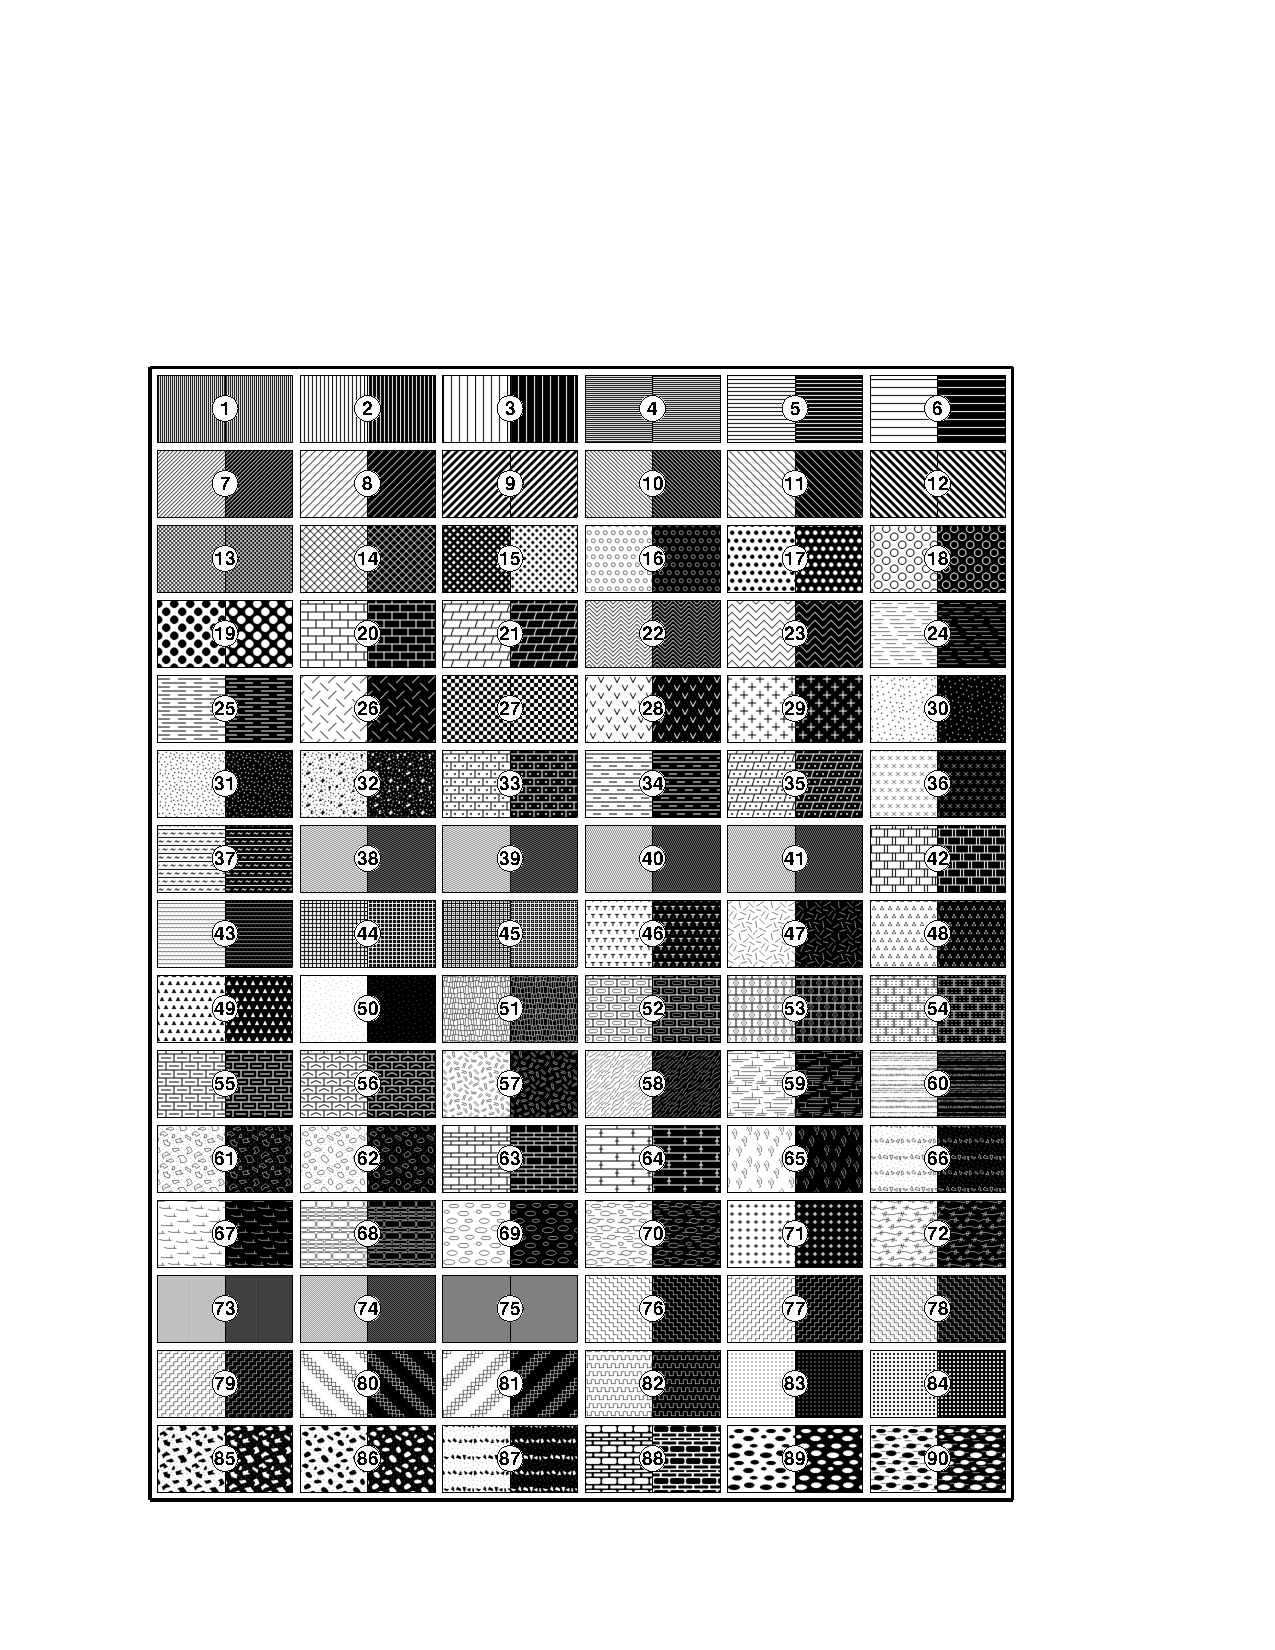
\includegraphics{scripts/GMT_App_E}
\end{center}

%------------------------------------------
%	$Id: GMT_Appendix_F.tex,v 1.1.1.1 2000-12-28 01:23:45 gmt Exp $
%
%	The GMT Documentation Project
%	Copyright 2000-2001.
%	Paul Wessel and Walter H. F. Smith
%------------------------------------------
%
\chapter{Chart of octal codes for characters}
\index{Characters!octal}
\index{Octal characters}
\thispagestyle{headings}

\GMTfig[h]{GMT_App_F_1}{Octal codes and corresponding symbols for standard fonts}

The characters and their octal codes in the reencoded standard fonts
are shown in Figure~\ref{fig:GMT_App_F_1}.  The chart for
the Symbol (\GMT\ font number 12) character
sets are presented in Figure~\ref{fig:GMT_App_F_2} below.  Gray
areas signify codes reserved for
control characters.  The octal code is obtained by appending the
column value to the $\backslash$?? value, e.g., $\partial$ is
$\backslash$266 in the Symbol font.  In order to use all the extended
characters you need to set {\bf WANT\_EURO\_FONT} to true in your
\filename{.gmtdefaults} file\footnote{By default, this is true if you chose
SI units and false if you chose US units during the installation.}.
\index{Symbol font}
\index{Font!symbol}

\GMTfig[h]{GMT_App_F_2}{Octal codes and corresponding symbols for the Symbol font}

The Pifont ZapfDingbats is available as \GMT\ font number 34 and
can be used for special symbols not listed above.  The various
symbols are illustrated in Figure~\ref{fig:GMT_App_F_3}.

\GMTfig[h]{GMT_App_F_3}{Octal codes and corresponding symbols for ZapfDingbats font}

%------------------------------------------
%	$Id$
%
%	The GMT Documentation Project
%	Copyright (c) 2000-2011.
%	P. Wessel, W. H. F. Smith, R. Scharroo, and J. Luis
%------------------------------------------
%
\chapter{\PS\ fonts used by \gmt}
\label{app:G}
\index{Font!standard}
\thispagestyle{headings}

\GMT\ uses the standard 35 fonts that come with most \PS\
laserwriters.  If your printer does not support some of these
fonts, it will automatically substitute the default font (which is
usually Courier).  The following is
a list of the \GMT\ fonts: \\

\GMTfig[h]{GMT_App_G}{The standard 35 \PS\ fonts recognized by \gmt.}

For the special fonts Symbol (12) and ZapfDingbats (34), see the
octal charts in Appendix~\ref{app:F}.  When specifying fonts in
\GMT, you can either give the entire font name \emph{or} just the
font number listed in this table.  To change the fonts used in
plotting basemap frames, see the man page for
\GMTprog{gmt.conf}.  For direct plotting of text-strings, see
the man page for \GMTprog{pstext}.


\section{Using non-default fonts with \GMT}
\label{sec:non-default-fonts}

To add additional fonts that you may have purchased or that are
available freely in the internet or at your institution, see the
instructions in the \filename{CUSTOM\_font\_info.d} under the
\filename{share/pslib} directory and continue reading.
%
\GMT\ does not read or process any font files and thus does not
know anything about installed fonts and their metrics. In order to
use extra fonts in \GMT\ you need to specify the \PS\ name of the
relevant fonts in the file \filename{CUSTOM\_font\_info.d}. You
can either edit the existing file distributed with \GMT\ to make
the changes global or you can create a new file in the current
working directory, e.g.:
%
\begin{verbatim}
LinBiolinumO      0.700    0
LinLibertineOB    0.700    0
\end{verbatim}
%
The format is a space delimited list of the \PS\ font name, the
font height-point size-ratio, and a boolean variable that tells
\GMT\ to re-encode the font (if set to zero). The latter has to be
set to zero as additional fonts will most likely not come in
standard \PS\ encoding. \GMT\ determines how tall typical
annotations might be from the font size ratio so that the vertical
position of labels and titles can be adjusted to a more uniform
typesetting. Now, you can set the \GMT\ font parameters to your
non-standard fonts:
%
\begin{verbatim}
gmtset FONT LinBiolinumO \
 FONT_TITLE 28p,LinLibertineOB \
 PS_CHAR_ENCODING ISO-8859-1 \
 MAP_DEGREE_SYMBOL degree
\end{verbatim}
%
After setting the encoding and the degree symbol, the
configuration part for \GMT\ is finished and you can proceed to
create \GMT-maps as usual. An example script is discussed in
Section~\ref{sec:non-default-fonts-example}.


\subsection{Embedding fonts in PostScript and PDF}

If you have Type 1 fonts in PFA (Printer Font ASCII) format you
can embed them directly by copying them at the very top of your
\PS-file, before even the \%!PS header comment. PFB (Printer Font
Binary), TrueType or OpenType fonts cannot be embedded in \PS\
directly and therefore have to be converted to PFA first.

However, you most likely will have to tell \progname{Ghostscript}
where to find your custom fonts in order to convert your
\GMT-\PS-plot to PDF or an image with \GMTprog{ps2raster}. When
you have used the correct \PS-names of the fonts in
\filename{CUSTOM\_font\_info.d} you only need to point the
\verb#GS_FONTPATH# environment variable to the directory where the
font files can be found and invoke \GMTprog{ps2raster} in the
usual way. Likewise you can specify \progname{Ghostscript}'s
\verb#-sFONTPATH# option on the command line with
\Opt[-sFONTPATH=/path/to/fontdir]{-C}.  \progname{Ghostscript},
which is invoked by \GMTprog{ps2raster}, does not depend on file
names. It will automatically find the relevant font files by their
\PS-names and embed and subset them in PDF-files. This is quite
convenient as the document can be displayed and printed even on
other computers when the font is not available locally. There is
no need to convert your fonts as \progname{Ghostscript} can handle
all Type 1, TrueType and OpenType fonts. Note also, that you do
not need to edit \progname{Ghostscript}'s Fontmap.GS.

If you do not want or cannot embed the fonts you can convert them
to outlines (shapes with fills) with \progname{Ghostscript} in the
following way:
\begin{verbatim}
gs -q -dNOCACHE -dSAFER -dNOPAUSE -dBATCH -dNOPLATFONTS \
  -sDEVICE=pswrite -sFONTPATH="/path/to/fontdir" \
  -sOutputFile=mapWithOutlinedFonts.ps map.ps
\end{verbatim}
Note, that this only works with the \emph{pswrite} device. If you
need outlined fonts in PDF, create the PDF from the converted
\PS-file.  Also, \GMTprog{ps2raster} cannot correctly crop
\progname{Ghostscript} converted \PS-files anymore. Use Heiko
Oberdiek's
\htmladdnormallinkfoot{\progname{pdfcrop}}{http://code.google.com/p/pdfcrop2/}
% \GMTprog{pdfcrop}
instead or crop with \GMTprog{ps2raster} \Opt{A} \Opt{Te} before
(See Example~\ref{sec:non-default-fonts-example}).


\subsection{Character encoding}

Since \PS\ itself does not support Unicode fonts, \progname{Ghostscript} will
re-encode the fonts on the fly. You have to make sure to set the
correct \verb#PS_CHAR_ENCODING# with gmtset and save your script
file with the same character encoding. Alternatively, you can
substitute all non ASCII characters with their corresponding octal
codes, e.g., \textbackslash 265 instead of \textmu. Note, that
\PS\ fonts support only a small range of glyphs and you may have
to switch the \verb#PS_CHAR_ENCODING# within your script.

%------------------------------------------
%	$Id: GMT_Appendix_H.tex,v 1.22 2011-04-07 00:55:30 guru Exp $
%
%	The GMT Documentation Project
%	Copyright (c) 2000-2011.
%	P. Wessel, W. H. F. Smith, R. Scharroo, and J. Luis
%------------------------------------------
%
\chapter{Problems with display of \gmt\ \PS}
\label{app:H}
\thispagestyle{headings}

\GMT\ creates valid (so far as we know) Adobe \PS\
Level 2.  It does not use operators specific to Level 3 and
should therefore produce output that should print on all \PS\ printers\footnote{Note, however, that the \Opt{Q} option in \GMTprog{grdimage}
will exercise a \PS\ Level 3 feature called colormasking.}.  Sometimes unexpected things
happen when \GMT\ output is sent to certain printers or displays.
This section lists some things we have learned from experience,
and some work-arounds.  Note that many of these lessons are now rather old so hopefully
these workarounds no longer apply to anybody...

\section{\PS\ driver bugs}
\index{PostScript@\PS!driver bugs}

When you try to display a \PS\ file on a device,
such as a printer or your screen, then a program called a
\PS\ device driver has to compute which device
pixels should receive which colors (black or white in the case
of a simple laser printer) in order to display the file.  At
this stage, certain device-dependent things may happen.  These
are not limitations of \GMT\ or \PS, but of the
particular display device.  The following bugs are known to us
based on our experiences:

\begin{enumerate}
\index{PostScript@\PS!Sun SPARCprinter bug}

\item 	Early versions of the Sun SPARCprinter software
caused linewidth-dependent path displacement.  We reported
this bug and it has been fixed in newer versions of the software.
Try using \GMTprog{psxy} to draw $y = f(x)$ twice, once with a
thin pen (\Opt{W}1) and once with a fat pen (\Opt{W}10);
if they do not plot on top of each other, you have this kind
of bug and need new software.  The problem may also show up
when you plot a mixture of solid and dashed (or dotted) lines
of various pen thickness

\index{PostScript@\PS!HP Laserjet 4M bug}

\item The first version of the HP Laserjet 4M (prior to Aug--93)
had bugs in the driver program.  The old one was
\PS\ SIMM, part number C2080-60001; the new one
is called \PS\ SIMM, part number C2080-60002.
You need to get this one plugged into your printer if you have
an HP LaserJet 4M.

\index{PostScript@\PS!limitations|(}

\item Apple Laserwriters with the older versions of Apple's
\PS\ driver will give the error ``limitcheck''
and fail to plot when they encounter a path exceeding about
1000--1500 points.  Try to get a newer driver from Apple, but
if you can't do that, set the parameter MAX\_L1\_PATH to
1000--1500 or even smaller in the file \filename{src/pslib\_inc.h}
and recompile \GMT.  The number of points in a \PS\
path can be arbitrarily large, in principle; \GMT\ will only
create paths longer than MAX\_L1\_PATH if the path represents
a filled polygon or clipping path.  Line-drawings (no fill)
will be split so that no segment exceeds MAX\_L1\_PATH.
This means \GMTprog{psxy} \Opt{G} will issue a warning when you
plot a polygon with more than MAX\_L1\_PATH points in it.  It is
then your responsibility to split the large polygon into several
smaller segments.  If \GMTprog{pscoast} gives such warnings and the
file fails to plot you may have to select one of the lower
resolution databases  The path limitation exemplified by these
Apple printers is what makes the higher-resolution coastlines
for \GMTprog{pscoast} non-trivial:  such coastlines have to be
organized so that fill operations do not generate excessively
large paths.  Some HP \PS\ cartridges for the
Laserjet III also have trouble with paths exceeding 1500
points; they may successfully print the file, but it can take
all night!
\index{PostScript@\PS!limitations|)}

\index{PostScript@\PS!Sun pageview}

\item 8-bit color screen displays (and programs which use only
8-bits, even on 24-bit monitors, such as Sun's \progname{pageview} under
OpenWindows) may not dither cleverly, and so the color they show you
may not resemble the color your \PS\ file is asking
for.  Therefore, if you choose colors you like on the screen,
you may be surprised to find that your plot looks different on
the hardcopy printer or film writer.  The only thing you can
do is be aware of this, and make some test cases on your hardcopy
devices and compare them with the screen, until you get used
to this effect.  (Each hardcopy device is also a little
different, and so you will eventually find that you want to
tune your color choices for each device.)  The rgb color cube
in example 11 may help.

\item Some versions of Sun's OpenWindows program \progname{pageview}
have only a limited number of colors available; the number
can be increased somewhat by starting \progname{openwin} with the
option ``\texttt{openwin -cubesize large}''.

\item Finally, \progname{pageview} seem to have problems understanding
the \texttt{setpagedevice} operator.  We recommend you only use
\progname{pageview} on EPS files or use \progname{ghostview} instead.

\index{PostScript@\PS!CMYK and RGB|(}

\item Many color hardcopy devices use CMYK color systems. \GMT\
\PS\ uses RGB (even if your CPT files are using HSV).
The three coordinates of RGB space can be mapped into three
coordinates in CMY space, and in theory K (black) is superfluous.
But it is hard to get CMY inks to mix into a good black or gray,
so these printers supply a black ink as well, hence CMYK.  The
\PS\ driver for a CMYK printer should be smart
enough to compute what portion of CMY can be drawn in K, and
use K for this and remove it from CMY; however, some of them
aren't.

\item In early releases of \GMT\ we always used the \PS\
command \texttt{r g b setrgbcolor} to specify colors, even if the color
happened to be a shade of gray ($r=g=b$) or black ($r=g=b=0$).  One
of our users found that black came out muddy brown when he used
\progname{FreedomOfPress} to make a Versatec plot of a \GMT\ map.
He found that if he used the \PS\ command \texttt{g setgray} (where $g$
is a graylevel) then the problem went away.
Apparently, his installation of \progname{FreedomOfPress} uses only CMY with
the command \texttt{setrgbcolor}, and so \texttt{0 0 0 setrgbcolor}
tries to make black out of CMY instead of K.  To fix this, in
release 2.1 of \GMT\ we changed some routines in \filename{pslib.c}
to check if ($r=g$ and $r=b$), in which case \texttt{g setgray} is
used instead of \texttt{r g b setrgbcolor}.

\item Recent experience with some Tektronix Phaser printers and
with commercial printing shops has shown that this substitution
creates problems precisely opposite of the problems our Versatec
user has.  The Tektronix and commercial (we think it was a Scitex)
machines do not use K when you say \texttt{0 setgray} but they do when
you say \texttt{0 0 0 setrgbcolor}.  We believe that these problems are
likely to disappear as the various software developers make their
codes more robust.  Note that this is not a fault with \GMT:
$r = g = b = 0$ means black and should plot that way.
Thus, the \GMT\ source code as shipped to you checks whether $r=g$
and $r=b$, in which case it uses \texttt{setgray}, else \texttt{setrgbcolor}.
If your gray tones are not being drawn with K, you have two
work-around options: (1) edit the source for \filename{pslib.c}
or (2) edit your \PS\ file and try using \texttt{setrgbcolor}
in all cases.  The simplest way to do so is to redefine the
\texttt{setgray} operator to use \texttt{setrgbcolor}.
Insert the line \\

\indent \texttt{/setgray  \{dup dup setrgbcolor\} def} \\

immediately following the first line in the file (starts with
\%!PS.) 

\item Some color film writers are very sensitive to the brand
of film.  If black doesn't look black on your color slides, try
a different film.
\index{PostScript@\PS!CMYK and RGB|)}

\end{enumerate}

\section{Resolution and dots per inch}
\index{PostScript@\PS!resolution and dpi}

The parameter \textbf{PS\_DPI} can be set by the user through
the \filename{gmt.conf} file or \GMTprog{gmtset}.  By default
it is equal to the value in the \filename{gmt\_defaults.h}
file, which is supplied with 300 when you get \GMT\ from us.
This seems a good size for most applications, but should ideally
reflect the resolution of your hardcopy device (most laserwriters
have at least 300 dpi, hence our default value).  \GMT\ computes what the
plot should look like in double precision floating point
coordinates, and then converts these to integer coordinates at
\textbf{PS\_DPI} resolution.  This helps us find out that certain
points in a path lie on top of other points, and we can remove
these, making smaller paths.  Small paths are important for the
laserwriter bugs above, and also to make fill operations compute
faster.  Some users have set their \textbf{PS\_DPI} to very large
numbers.  This only makes the \PS\ output bigger
without affecting the appearance of the plot.  However, if you
want to make a plot which fits on a page at first, and then
later magnify this same \PS\ file to a huge size,
the higher DPI is important.  Your data may not have the higher
resolution but on certain devices the edges of fonts will not
look crisp if they are not drawn with an effective resolution
of 300 dpi or so.  Beware of making an excessively large path.
Note that if you change dpi the linewidths produced by your
\Opt{W} options will change, unless you have appended {\bf p}
for linewidth in points.

\section{European characters}
\index{Text!European}
\index{Characters!European}
Note for users of \progname{pageview} in Sun OpenWindows: \GMT\ now
offers some octal escape sequences to load European alphabet
characters in text strings (see Section~\ref{sec:escape}).  When
this feature is enabled, the header on \GMT\ \PS\ output includes
a section defining special fonts.  The definition is added to
the header whether or not your plot actually uses the fonts.

Users who view their \GMT\ \PS\ output using
\progname{pageview} in OpenWindows on Sun computers or user older
laserwriters may have difficulties with the European font
definition.  If your installation of OpenWindows followed
a space-saving suggestion of Sun, you may have excluded the
European fonts, in which case \progname{pageview} will fail
to render your plot.

Ask your system administrator about this, or run this simple
test: (1) View a \GMT\ \PS\ file with \progname{pageview}.
If it comes up OK, you will be fine.  If it comes up blank,
open the ``Edit PostScript'' button and examine the lower
window for error messages.  (The European font problem generates
lots of error messages in this window).  (2)  Verify that the
\PS\ file is OK, by sending it to a laserwriter
and making sure it comes out.  (3)  If the \PS\
file is OK but it chokes \progname{pageview}, then edit the \PS\
file, cutting out everything between the lines: \\

\noindent
\%\%\%\%\% START OF EUROPEAN FONT DEFINITION \%\%\%\%\% \\
$<$bunch of definitions$>$ \\
\%\%\%\%\% END OF EUROPEAN FONT DEFINITION \%\%\%\%\% \\

Now try \progname{pageview} on the edited version.  If it now comes
up, you have a limited subset of OpenWindows installed.  If
you discover that these fonts cause you trouble, then you can
edit your \filename{gmt.conf} file to set \textbf{PS\_CHAR\_ENCODING} = Standard,
which will suppress the printing of this definition in the
\GMT\ \PS\ header.  You can
make output which will be viewable in \progname{pageview} without
any editing.  However, you would have to reset this to TRUE
before attempting to use European fonts, and then the output will
become un-\progname{pageview}-able again.  If you try to
concatenate segments of \GMT\ \PS\ made with and without the
European fonts enabled, then you may find that you have problems,
either with the definition, or because you ask for something
not defined.

\section{Hints}
\index{PostScript@\PS!\GMT\ hints}

When making images and perspective views of large amounts of
data, the \GMT\ programs can take some time to run, the resulting
\PS\ files can be very large, and the time to display
the plot can be long.  Fine tuning a plot script can take lots
of trial and error.  We recommend using \GMTprog{grdsample} to make
a low resolution version of the data files you are plotting, and
practice with that, so it is faster; when the script is perfect,
use the full-resolution data files.  We often begin building a
script using only \GMTprog{psbasemap} or \GMTprog{pscoast} to get
the various plots oriented correctly on the page; once this works
we replace the \GMTprog{psbasemap} calls with the actually desired
\GMT\ programs.

If you want to make color shaded relief images and you haven't
had much experience with it, here is a good first cut at the
problem:  Set your \textbf{COLOR\_MODEL} to HSV using \GMTprog{gmtset}.  Use
\GMTprog{makecpt} or \GMTprog{grd2cpt} to make a continuous color
palette spanning the range of your data.  Use the \Opt{Nt}
option on \GMTprog{grdgradient}.  Try the result, and then play with
the tuning of the \filename{gmt.conf}, the CPT file, and
the gradient file.

%------------------------------------------
%	$Id: GMT_Appendix_I.tex,v 1.25 2011-02-28 16:05:16 remko Exp $
%
%	The GMT Documentation Project
%	Copyright 2000-2011.
%	Paul Wessel and Walter H. F. Smith
%------------------------------------------
%
\chapter{Color Space: The final frontier}
\label{app:I}
\thispagestyle{headings}

\index{Color|(}
\index{Color!HSV system|(}
\index{Color!RGB system|(}

In this Appendix, we are going to try to explain the relationship
between the RGB, CMYK, and HSV color systems so as to (hopefully) make
them more intuitive.  \GMT\ allows users to specify colors in cpt
files in either of these three systems. Interpolation between colors is performed in either RGB or HSV, depending on the specification in the cpt file. Below, we will explain why this all matters.

\section{RGB color system}
Remember your (parents') first color television set? Likely it had three little bright colored squares on it: red, green, and blue. And that is exactly what each color on the tube is made of: varying levels of red, green and blue light. Switch all of them off, $r=g=b=0$, then you have black. All of them at maximum, $r=g=b=255$, creates white. Your computer screen works the same way.

A mix of levels of red, green, and blue creates basically any color imaginable. In \GMT\ each color can be represented by the triplet $r$/$g$/$b$. For example, 127/255/0 (half red, full green, and no blue) creates a color called chartreuse. The color sliders in the graphics program \progname{GIMP} are an excellent way to experiment with colors, since they show you in advance how moving one of the color sliders will change the color. As Figure~\ref{fig:gimp}\emph{a} shows: increase the red and you will get a more yellow color, while lowering the blue level will turn it into brown.

\begin{figure}[b]
   \includegraphics[width=0.47\textwidth,bb=0 0 375 209]{fig/gimp-sliders.png}~\emph{a}\hfill
   \emph{b}~\includegraphics[width=0.47\textwidth,bb=0 0 375 209]{fig/gimp-panel.png}
   \caption{Chartreuse in \protect\progname{GIMP}. (\emph{a}) Sliders indicate how the color is altered when changing the H, S, V, R, G, or B levels. (\emph{b}) For a constant hue (here 90\DS) value increases to the right and saturation increases up, so the ``pure'' color is on the top right.}
   \label{fig:gimp}
\end{figure}

Is chocolate your favorite color, but you do not know the RGB equivalent values? Then look them up in Figure~\ref{fig:RGBchart} or type \progname{man gmtcolors} for a full list. It's 210/105/30. But \GMT\ makes it easy on you: you can specify pen, fill, and palette colors by any of the more than 500 unique colors found in that file.

Are you very web-savvy and work best with hexadecimal color codes as they are used in HTML? Even that is allowed in \GMT. Just start with a hash mark (\texttt{\#}) and follow with the 2 hexadecimal characters for red, green, and blue. For example, you can use \texttt{\#79ff00} for chartreuse, \texttt{\#D2691E} for chocolate.

\begin{figure}
   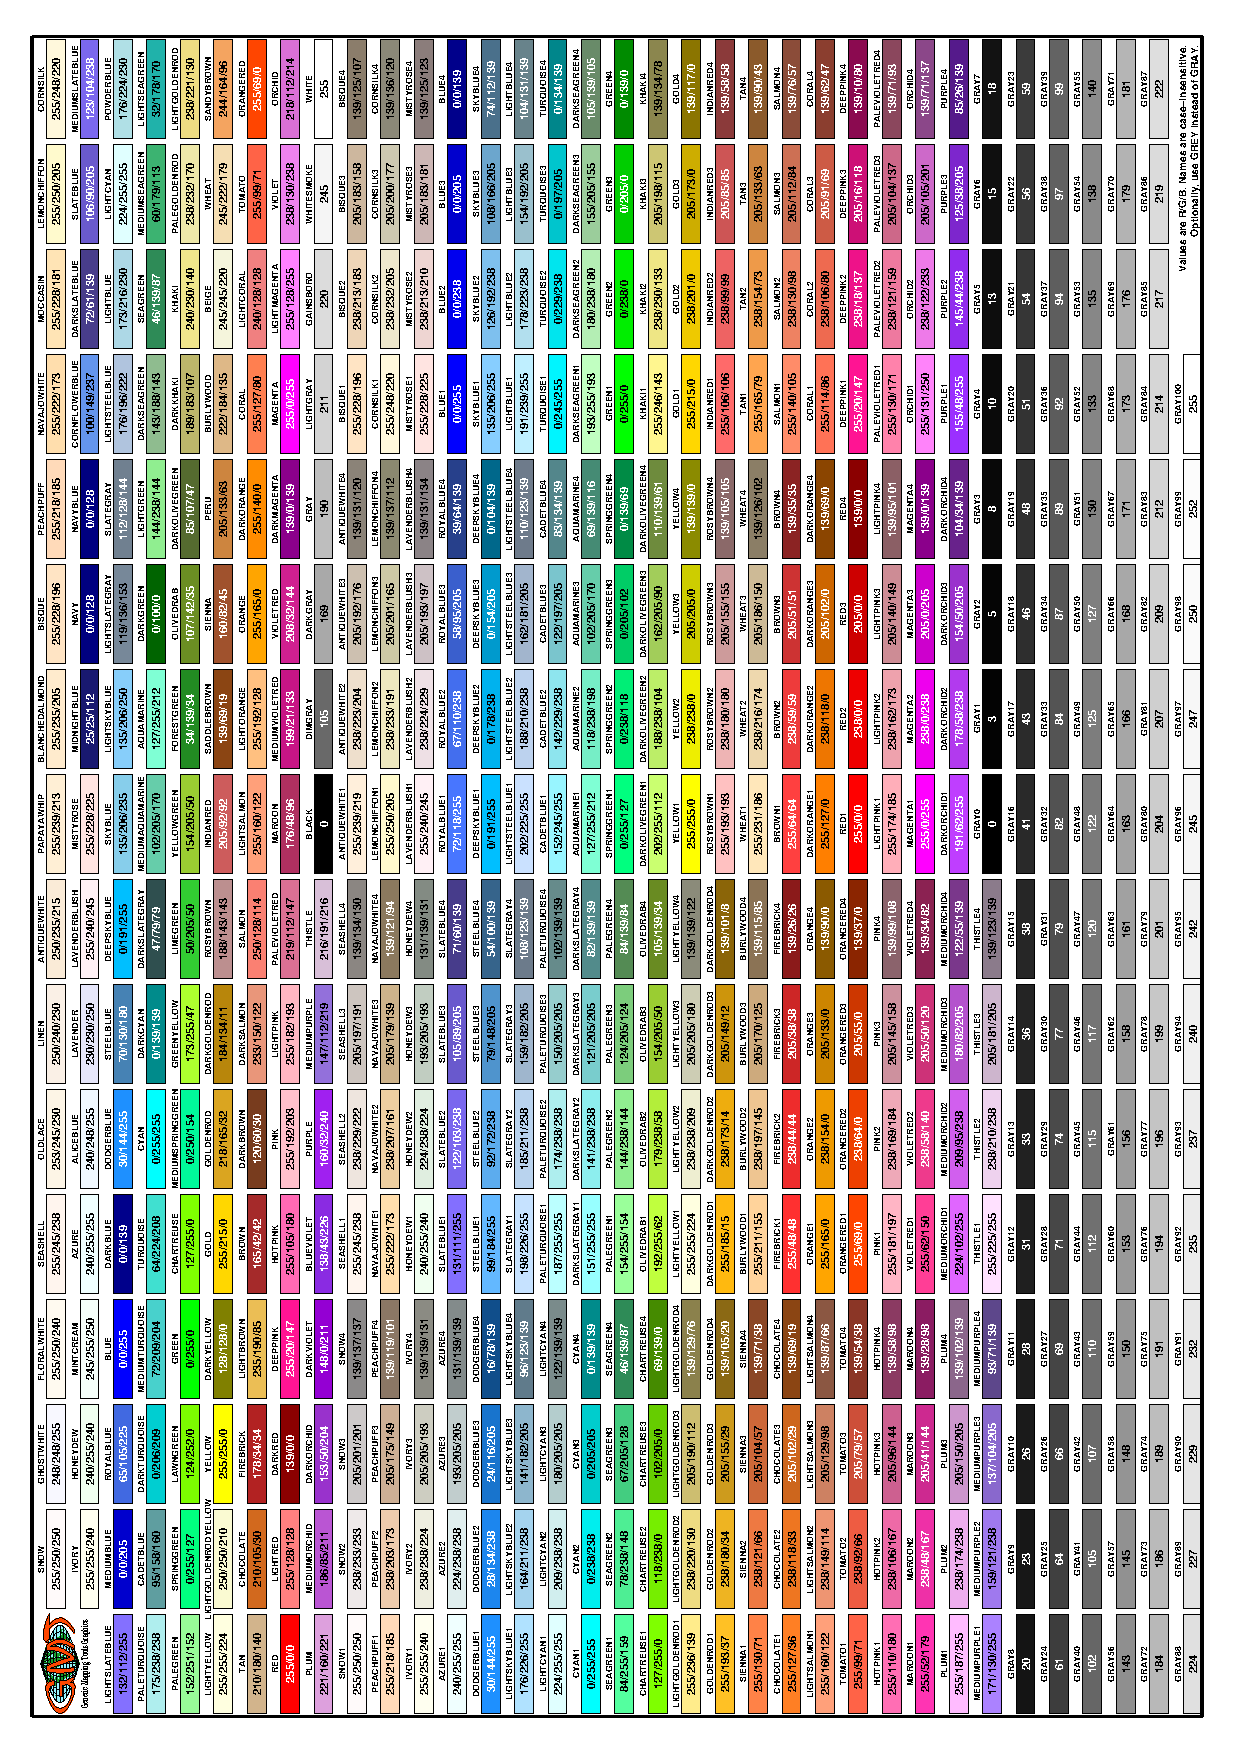
\includegraphics[angle=90,width=\textwidth]{scripts/GMT_RGBchart_a4}
   \caption{The 555 unique color names that can be used in GMT. Lower, upper, or mixed case, as well as the british
   spelling of ``grey'' are allowed. A4, Letter, and Tabloid sized versions of this RGB chart can be found in the
   GMT documentation directory.}
   \label{fig:RGBchart}
\end{figure}

\section{HSV color system}
If you have played around with RGB color sliders, you will have noticed that it is not intuitive to make a chosen color lighter or darker, more saturated or more gray. It would involve changing three sliders. To make it easier to manipulate colors in terms of lightness and saturation, another coordinate system was invented: HSV (hue, saturation, value). Those terms can be made clear best by looking at the color sliders in Figure~\ref{fig:gimp}\emph{a}. Hue (running from 0\DS\ to 360\DS) gives you the full spectrum of saturated colors. Saturation (from 0 to 1, or 100\%) tells you how `full' your color is: reduce it to zero and you only have gray scales. Value (from 0 to 1, or 100\%) will bring you from black to a fully saturated color. Note that ``value'' is not the same as ``intensity'', or ``lightness'', used in other color geometries. ``Brilliance'' may be the best alternative word to describe ``value''. Apple calls it as ``brightness'', and hence refers to HSB for this color space.

Want more chartreuse or chocolate? You can specify them in \GMT\ as 90-1-1 and 25-0.86-0.82, respectively.

\section{The color cube}
We are going to try to give you a geometric picture of color
mixing in RGB and HSV by means of a tour of the RGB cube depicted in Figure~\ref{fig:GMT_example_11}.  The geometric
picture is most helpful, we think, since HSV are not orthogonal
coordinates and not found from RGB by a simple algebraic transformation.
So here goes: Look at the
cube face with black, red, magenta, and blue corners.
This is the $g$ = 0 face.  Orient the cube so that you are
looking at this face with black in the lower left corner.  Now
imagine a right-handed cartesian ($r$,$g$,$b$) coordinate system
with origin at the black point; you are looking at the $g = 0$
plane with $r$ increasing to your right, $g$ increasing
away from you, and $b$ increasing up.  Keep this sense of
($r$,$g$,$b$) as you look at the cube.

Now tip the cube such that the black corner faces down and the white corner up. When looking from the top, you can see the hue, contoured in gray solid lines, running around in 360\DS\ counter-clockwise. It starts with shades of red (0\DS), then goes through green (120\DS) and blue (240\DS), back to red.

On the three faces that are now on the lower side (with the white print) one of ($r$,$g$,$b$) is equal to 0. These three faces meet at the black corner, where $r = g = b = 0$. On these three faces the colors are fully saturated: $s$ = 1. The dashed white lines indicate different levels of $v$, ranging from 0 to 1 with contours every 0.1.

On the upper three faces (with the black print), one of ($r$,$g$,$b$) is equal to the
maximum value.  These three faces meet at the white corner, where
$r = g = b = 255$.  On these three faces value is at
its maximum: $v$ = 1 (or 100\%). The dashed black lines indicate varying levels of saturation: $s$ ranges from 0 to
1 with contours every 0.1.

Now turn the cube around on its vertical axis (running from the black to the white corner). Along the six edges that zigzag around the ``equator'', both saturation and value are maximum, so $s = v = 1$. Twirling the cube around and tracing the zigzag, you will visit six of the eight corners of the
cube, with changing hue ($h$):  red (0\DS), yellow (60\DS), green
(120\DS), cyan (180\DS), blue (240\DS), and magenta
(300\DS). Three of these are the RGB colors; the other three
are the CMY colors which are the complement of RGB and are used in many
color hardcopy devices (see below).  The only cube
corners you did not visit on this path are the black and white corners.
They lie on the vertical axis where hue is undefined and $r = g = b$. Any point on this axis is a shade of gray.

Let us call the points where $s = v = 1$ (points along the RYGCBM path described above) the ``pure'' colors.  If we start at a pure color
and we want to whiten it, we can keep $h$ constant and $v = 1$
while decreasing $s$; this will move us along one of the cube
faces toward the white point.  If we start at a pure color and we want
to blacken it, we can keep $h$ constant and $s = 1$ while decreasing
$v$; this will move us along one of the cube faces toward the black
point.  Any point in ($r$,$g$,$b$) space which can be thought of as a
mixture of pure color + white, or pure color + black, is on a face of
the cube.

The points in the interior of the cube are a little harder to describe.
The definition for $h$ above works at all points in (non-gray)
($r$,$g$,$b$) space, but so far we have only looked at ($s$,
$v$) on the cube faces, not inside it.  At interior points, none
of ($r$,$g$,$b$) is equal to either 0 or 255.  Choose such a point,
not on the gray axis.  Now draw a line through your point so that the
line intersects the gray axis and also intersects the RYGCBM path of
edges somewhere.  It is always possible to construct this line, and
all points on this line have the same hue.  This construction shows
that any point in RGB space can be thought of as a mixture of a pure
color plus a shade of gray.  If we move along this line away from the
gray axis toward the pure color, we are ``purifying'' the color by
``removing gray''; this move increases the color's saturation.  When
we get to the point where we cannot remove any more gray, at least one
of ($r$,$g$,$b$) will have become zero and the color is now fully
saturated; $s = 1$.  Conversely, any point on the gray axis is
completely undersaturated, so that $s = 0$ there.  Now we see that
the black point is special, $s$ is both 0 and 1 at the same time. In other words, at the black point saturation in undefined (and so is hue). The convention is to use $h = s = v = 0$ at this point.

It remains to define value. To do so, try this:
Take your point in RGB space and construct a line through it so that
this line goes through the black point; produce this line from black
past your point until it hits a face on which $v = 1$.  All points
on this line have the same hue.  Note that this line and the line we
made in the previous paragraph are both contained in the plane whose
hue is constant.  These two lines meet at some arbitrary
angle which varies depending on which point you chose.  Thus HSV is
not an orthogonal coordinate system.  If the line you made in the
previous paragraph happened to touch the gray axis at the black point,
then these two lines are the same line, which is why the black point
is special.  Now, the line we made in this paragraph illustrates the
following:  If your chosen point is not already at the end of the
line, where $v = 1$, then it is possible to move along the line in
that direction so as to increase ($r$,$g$,$b$) while keeping the
same hue.  The effect this has on a color monitor is to make the
color more ``brilliant'', your hue will become ``stronger''; if you are already on a plane where
at least one of ($r$,$g$,$b$) = 255, then you cannot get a stronger
version of the same hue.  Thus, $v$ measures brilliance or strength.  Note that
it is not quite true to say that $v$ measures distance away from
the black point, because $v$ is not equal to $\sqrt{r^2 + g^2 + b^2}/255$.

Another representation of the HSV space is the color cone illustrated in Figure~\ref{fig:hsv-cone}.

\begin{figure}[h]
   \parbox[b]{0.54\textwidth}{``Pure'' colors are around the edge of the circular surface at the top. Hue runs counter-clockwise. Saturation decreases to the center. Value increases from zero (black) at the bottom to 1 at the top. Gray shades are along the vertical axis.}%
   \hfill%
   \includegraphics[width=0.45\textwidth,bb=0 0 750 508]{fig/hsv-cone.png}%
   \caption{The HSV color space.}
   \label{fig:hsv-cone}
\end{figure}

\section{Color interpolation}
\index{Color!interpolation}
From studying the RGB cube, we hope you will have understood that there are different routes to follow between two colors, depending whether you are in the RGB or HSV system. Suppose you would make an interpolation between blue and red. In the RGB system you would follow a path diagonally across a face of the cube, from 0/0/255 (blue) via 127/0/127 (purple) to 255/0/0 (red). In the HSV system, you would trace two edges, from 240-1-1 (blue) via 300-1-1 (magenta) to 360-1-1 (red). That is even assuming software would be smart enough to go the shorter route. More likely, red will be recorded as 0-1-1, so hue will be interpolated the other way around, reducing hue from 240\DS\ to 0\DS, via cyan, green, and yellow.

Depending on the design of your color palette, you may want to have it either way. By default, \GMT\ interpolates in RGB space, even when the original color palette is in the HSV system. However, when you add the line \texttt{\#COLOR\_MODEL=+HSV} (with the leading `+' sign) in the header of the color palette file, \GMT\ will not only read the color representation as HSV values, but also interpolate colors in the HSV system. That means that H, S, and V values are interpolated linearly between two colors, instead of their respective R, G, and B values.

The top row in Figure~\ref{fig:GMT_color_interpolate} illustrates two examples: a blue-white-red scale (the \textsf{polar} palette in Appendix~\ref{app:M}) interpolated in RGB and the \textsf{rainbow} palette interpolated in HSV. The bottom row of the Figure demonstrates how things can go terribly wrong when you do the interpolation in the other system.

\begin{figure}[h]
   \centering
   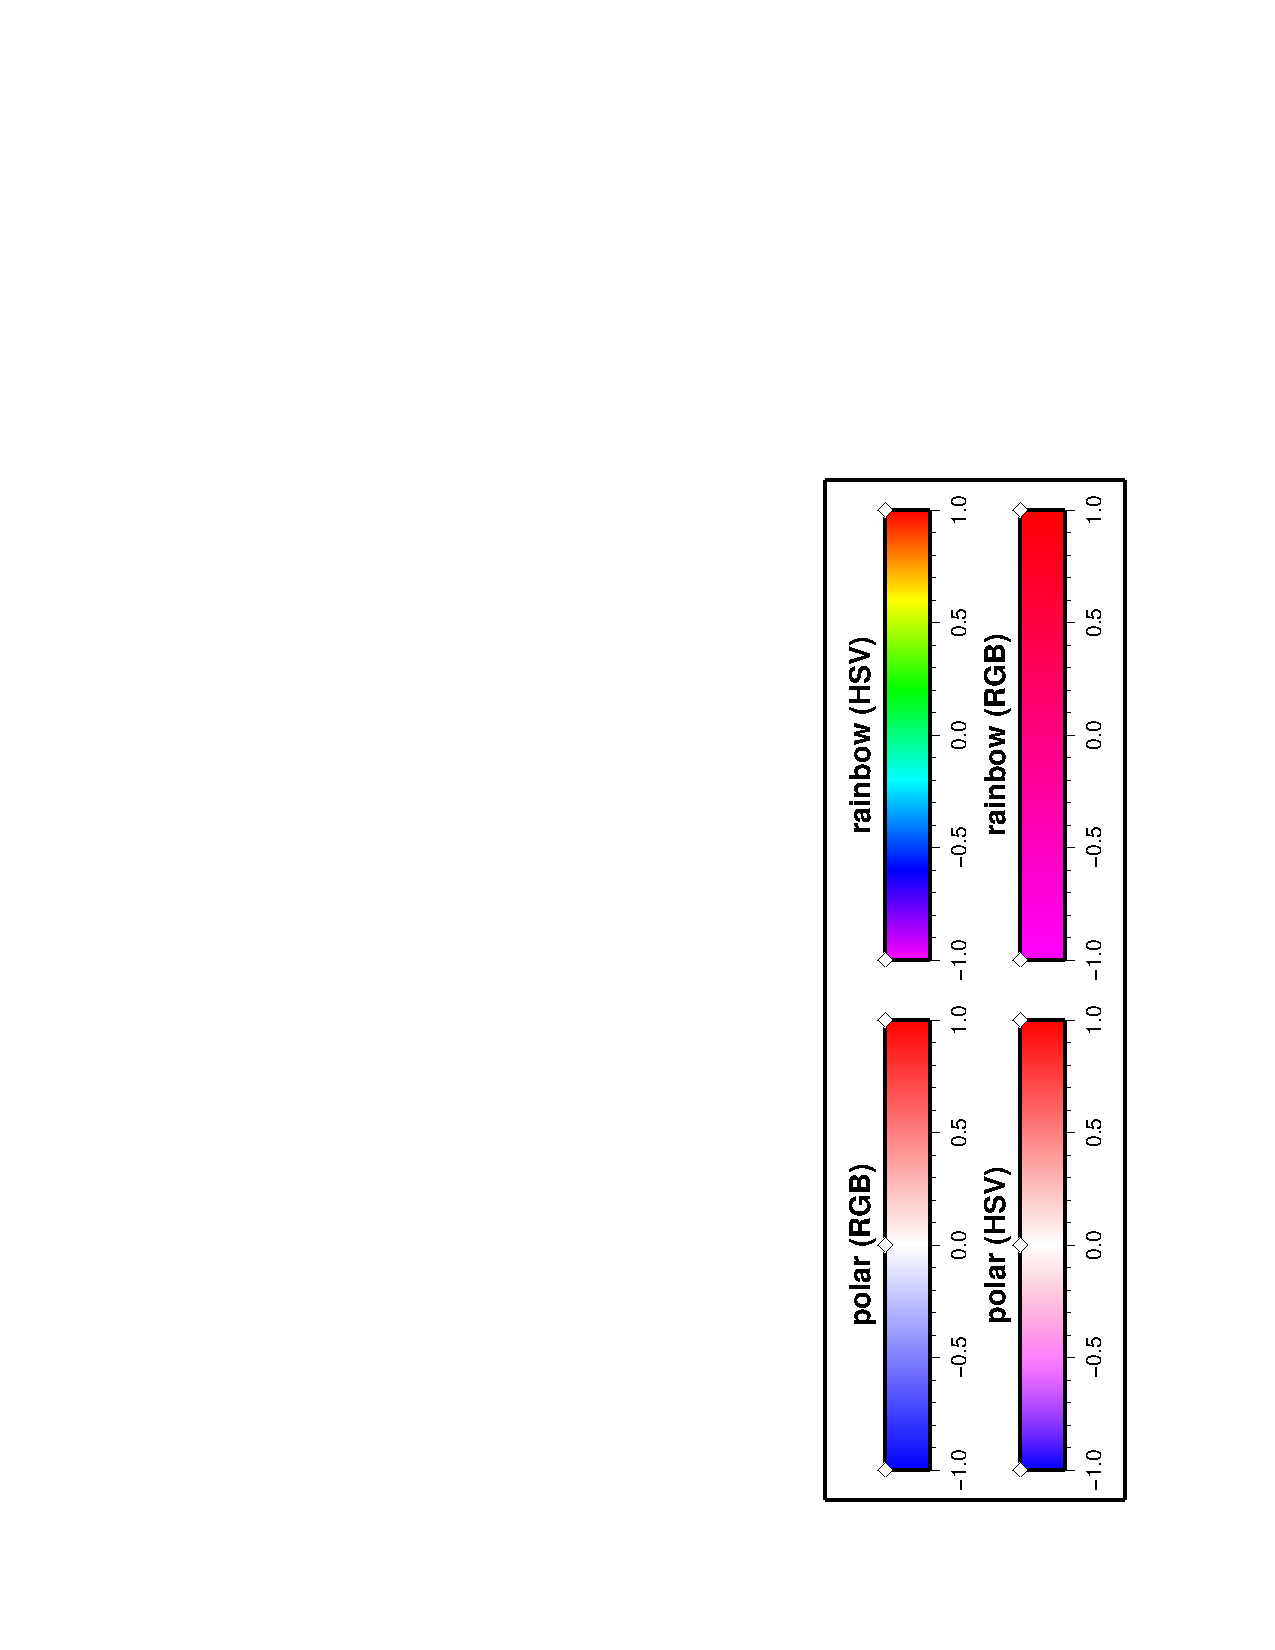
\includegraphics[width=0.80\textwidth]{scripts/GMT_color_interpolate}%
   \caption{When interpolating colors, the color system matters. The polar palette on the left needs to be interpolated in RGB, otherwise hue will change between blue (240\DS) and white (0\DS). The rainbow palette should be interpolated in HSV, since only hue should change between magenta (300\DS) and red (0\DS). Diamonds indicate which colors are defined in the palettes; they are fixed, the rest is interpolated.}
   \label{fig:GMT_color_interpolate}
\end{figure}

\section{Artificial illumination}
\index{Illumination, artificial}
\index{Artificial illumination}
\GMT\ uses the HSV system to
achieve artificial illumination of colored images (e.g. \Opt{I}
option in \GMTprog{grdimage}) by changing the saturation \emph{s} and value \emph{v}
coordinates of the color.  When the intensity is zero (flat illumination), the data
are colored according to the cpt file.  If the intensity is
non-zero, the color is either lightened or darkened depending on the illumination.
The color is first converted to HSV (if necessary) and then
darkened by moving ($s$,$v$) toward (\textbf{HSV\_MIN\_SATURATION},
\textbf{HSV\_MIN\_VALUE}) if the intensity is negative, or lightened by sliding ($s$,$v$) toward
(\textbf{HSV\_MAX\_SATURATION}, \textbf{HSV\_MAX\_VALUE}) if the illumination is positive.
The extremes of the $s$ and $v$ are defined in the \filename{.gmtdefaults4} file and are usually
chosen so the corresponding points are nearly black ($s$ = 1,
$v$ = 0) and white ($s$ = 0, $v$ = 1).
The reason this works is that the HSV system allows movements in
color space which correspond more closely to what we mean by
``tint'' and ``shade''; an instruction like ``add white'' is
easy in HSV and not so obvious in RGB.

\section{Thinking in RGB or HSV}
The RGB system is understandable because it is cartesian, and we all
learned cartesian coordinates in school.  But it doesn't help us
create a tint or shade of a color; we cannot say, ``We want orange,
and a lighter shade of orange, or a less vivid orange''.  With HSV we
can do this, by saying, ``Orange must be between red and yellow, so
its hue is about $h$ = 30\DS; a less vivid orange has a lesser
$s$, a darker orange has a lesser $v$''.  On the other hand,
the HSV system is a peculiar geometric construction, more like a cone (Figure~\ref{fig:hsv-cone}). It is not an
orthogonal coordinate system, and it is not found by a matrix
transformation of RGB; these make it difficult in some cases too.
Note that a move toward black or a move toward white will change both
$s$ and $v$, in the general case of an interior point in the
cube. The HSV system also doesn't behave well for very dark colors,
where the gray point is near black and the two lines we constructed
above are almost parallel.  If you are trying to create nice colors
for drawing chocolates, for example, you may be better off guessing
in RGB coordinates.
\index{Color!HSV system|)}
\index{Color!RGB system|)}

\section{CMYK color system}
\index{Color!CMYK system}
Finally, you can imagine that printers work in a different way: they mix different paints to make a color. The more paint, the darker the color, which is the reverse of adding more light. Also, mixing more colored paints does not give you true black, so that means that you really need four colors to do it right. Open up your color printer and you'll probably find four cartridges: cyan, magenta, yellow (often these are combined into one), and black. They form the CMYK system of colors, each value running from 0 to 1 (or 100\%). In \GMT\ CMYK color coding can be achieved using $c$/$m$/$y$/$k$ quadruplets.

Obviously, there is no unique way to go from the 3-dimensional RGB system to the 4-dimensional CMYK system. So, again, there is a lot of hand waving applied in the transformation. Strikingly, CMYK actually covers a smaller color space than RGB. We will not try to explain you the details behind it, just know that there is a transformation needed to go from the colors on your screen to the colors on your printer. It might explain why what you see is not necessarily what you get. If you are really concerned about how your color plots will show up in your PhD thesis, for example, it might be worth trying to save and print all your color plots using the CMYK system. Letting \GMT\ do the conversion to CMYK may avoid
some nasty surprises when it comes down to printing. To specify the color space of your \PS\ file, set \textbf{PS\_COLOR} in the \filename{.gmtdefaults4} file to RGB, HSV, or CMYK.
\index{Color|)}

%------------------------------------------
%	$Id: GMT_Appendix_J.tex,v 1.17 2011-05-18 22:23:49 remko Exp $
%
%	The GMT Documentation Project
%	Copyright (c) 2000-2011.
%	P. Wessel, W. H. F. Smith, R. Scharroo, and J. Luis
%------------------------------------------
%
\chapter{Filtering of data in \gmt}
\label{app:J}
\thispagestyle{headings}

The \GMT\ programs \GMTprog{filter1d} (for tables of data indexed
to one independent variable) and \GMTprog{grdfilter} (for data
given as 2-dimensional grids) allow filtering of data by a
moving-window process.  (To filter a grid by Fourier transform use
\GMTprog{grdfft}.)  Both programs use an argument
\Opt{F}$<$\emph{type}$><$\emph{width}$>$ to specify the type of
process and the window's width (in 1-d) or diameter (in 2-d).
(In \GMTprog{filter1d} the width is a length of the time or
space ordinate axis, while in \GMTprog{grdfilter} it is the
diameter of a circular area whose distance unit is related to
the grid mesh via the \Opt{D} option). If the process is a
median, mode, or extreme value estimator then the window 
output cannot be written as a convolution and the filtering
operation is not a linear operator.  If the process is a weighted
average, as in the boxcar, cosine, and gaussian filter types, 
then linear operator theory applies to the filtering process.
These three filters can be described as convolutions with an
impulse response function, and their transfer functions 
can be used to describe how they alter components in the input
as a function of wavelength.

Impulse responses are shown here for the boxcar, cosine, and
gaussian filters.  Only the relative amplitudes of the filter
weights shown; the values in the center of the window have 
been fixed equal to 1 for ease of plotting.  In this way the
same graph can serve to illustrate both the 1-d and 2-d impulse
responses; in the 2-d case this plot is a diametrical
cross-section through the filter weights (Figure~\ref{fig:GMT_App_J_1}).

\GMTfig[H]{GMT_App_J_1}{Impulse responses for \gmt\ filters.}

Although the impulse responses look the same in 1-d and 2-d,
this is not true of the transfer functions; in 1-d the transfer
function is the Fourier transform of the impulse response, 
while in 2-d it is the Hankel transform of the impulse response.
These are shown in Figures~\ref{fig:GMT_App_J_2} and
\ref{fig:GMT_App_J_3}, respectively.  Note that in 1-d the boxcar transfer
function has its first zero crossing at $f = 1$, while in 2-d 
it is around $f \sim 1.2$.  The 1-d cosine transfer function
has its first zero crossing at $f = 2$; so a cosine filter needs
to be twice as wide as a boxcar filter in order to zero the same
lowest frequency.  As a general rule, the cosine and gaussian
filters are ``better'' in the sense that they do not have the
``side lobes'' (large-amplitude oscillations in the transfer
function) that the boxcar filter has.  However, they are
correspondingly ``worse'' in the sense that they require more
work (doubling the width to achieve the same cut-off wavelength).

\clearpage

\GMTfig[H]{GMT_App_J_2}{Transfer functions for 1-D \gmt\ filters.}

One of the nice things about the gaussian filter is that its
transfer functions are the same in 1-d and 2-d.  Another nice
property is that it has no negative side lobes.  There are many 
definitions of the gaussian filter in the literature (see page
7 of Bracewell\footnote{R. Bracewell, \emph{The Fourier Transform
and its Applications}, McGraw-Hill, London, 444p., 1965.}).  We
define $\sigma$ equal to 1/6 of the filter width, and the impulse
response proportional to $\exp[-0.5(t/\sigma)^2)$.  With this
definition, the transfer function is $\exp[-2(\pi\sigma f)^2]$
and the wavelength at which the transfer function equals 0.5 is 
about 5.34 $\sigma$, or about 0.89 of the filter width.

\GMTfig[H]{GMT_App_J_3}{Transfer functions for 2-D (radial) \gmt\ filters.}

%------------------------------------------
%	$Id: GMT_Appendix_K.tex,v 1.26 2011-07-16 00:10:38 guru Exp $
%
%	The GMT Documentation Project
%	Copyright (c) 2000-2011.
%	P. Wessel, W. H. F. Smith, R. Scharroo, and J. Luis
%------------------------------------------
%
\chapter{The \gmt\ High-Resolution Coastline Data}
\label{app:K}
\index{GMT@\GMT!coastlines|(}
\index{Coastlines!preprocessing|(}
\thispagestyle{headings}

Starting with version 3.0, \GMT\ use a completely new coastline
database and the \GMTprog{pscoast} utility was been completely
rewritten to handle the new file format.  Many users have asked
us why it has taken so long for \GMT\ to use a high-resolution
coastline database; after all, such data have been available in
the public domain for years.  To answer such questions we will
take you along the road that starts with these public domain
data sets and ends up with the database used by \GMT.

\section{Selecting the right data} 
\index{World Data Bank II}
\index{CIA Data Bank}
\index{World Vector Shoreline}
\index{WVS}
\index{WDBII}

There are two well-known public-domain data sets that could be
used for this purpose.  Once is known as the World Data Bank II
or CIA Data Bank (WDB) and contains coastlines, lakes, political
boundaries, and rivers.  The other, the World Vector Shoreline
(WVS) only contains shorelines between saltwater and land (i.e.,
no lakes).  It turns out that the WVS data is far superior to the
WDB data as far as data quality goes, but as noted it lacks lakes,
not to mention rivers and borders.  We decided to use the WVS
whenever possible and supplement it with WDB data.  We got these
data over the Internet; they are also available on CD-ROM from
the National Geophysical Data Center in Boulder, Colorado\footnote{
www.ngdc.noaa.gov}.

\section{Format required by \gmt} 

In order to paint continents or oceans it is necessary that the
coastline data be organized in polygons that may be filled.
Simple line segments can be used to draw the coastline, but for
painting polygons are required.  Both the WVS and WDB data
consists of unsorted line segments: there is no information
included that tells you which segments belong to the same
polygon (e.g., Australia should be one large polygon).
In addition, polygons enclosing land must be differentiated from
polygons enclosing lakes since they will need different paint.
Finally, we want \GMTprog{pscoast} to be flexible enough that it can
paint the land \emph{or} the oceans \emph{or} both.
If just land (or oceans) is selected we do not want to paint
those areas that are not land (or oceans) since previous plot
programs may have drawn in those areas.  Thus, we will need to
combine polygons into new polygons that lend themselves to fill
land (or oceans) only (Note that older versions of \GMTprog{pscoast}
always painted lakes and wiped out whatever was plotted beneath).

\section{The long and winding road} 

The WVS and WDB together represent more than 100 Mb of binary
data and something like 20 million data points.  Hence, it
becomes obvious that any manipulation of these data must be
automated.  For instance, the reasonable requirement that no
coastline should cross another coastline becomes a complicated
processing step.

\begin{enumerate} 

\item To begin, we first made sure that all data were ``clean'',
i.e. that there were no outliers and bad points.  We had to
write several programs to ensure data consistency and remove
``spikes'' and bad points from the raw data.  Also, crossing
segments were automatically ``trimmed'' provided only
a few points had to be deleted.  A few hundred more complicated
cases had to be examined semi-manually.

\item Programs were written to examine all the loose segments
and determine which segments should be joined to produce
polygons.  Because not all segments joined exactly (there were
non-zero gaps between some segments) we had to find all possible
combinations and choose the simplest combinations.
The WVS segments joined to produce more than 200,000 polygons,
the largest being the Africa-Eurasia polygon which has 1.4
million points.  The WDB data resulted in a smaller data base
($\sim$25\% of WVS).

\item We now needed to combine the WVS and WDB data bases.
The main problem here is that we have duplicates of polygons:
most of the features in WVS are also in WDB.  However, because
the resolution of the data differ it is nontrivial to figure
out which polygons in WDB to include and which ones to ignore.
We used two techniques to address this problem.
First, we looked for crossovers between all possible pairs of
polygons.  Because of the crossover processing in step 1 above we know
that there are no remaining crossovers within WVS and WDB; thus
any crossovers would be between WVS and WDB polygons.  Crossovers
could mean two things: (1) A slightly misplaced WDB polygon
crosses a more accurate WVS polygon, both representing the same
geographic feature, or (2) a misplaced WDB polygon (e.g. a small
coastal lake) crosses the accurate WVS shoreline.  We distinguished
between these cases by comparing the area and centroid of the two
polygons.  In almost all cases it was obvious when we had
duplicates; a few cases had to be checked manually.  Second,
on many occasions the WDB duplicate polygon did not cross its
WVS counterpart but was either entirely inside or outside the
WVS polygon.  In those cases we relied on the area-centroid tests.

\item While the largest polygons were easy to identify by visual
inspection, the majority remain unidentified.  Since it is
important to know whether a polygon is a continent or a small
pond inside an island inside a lake we wrote programs that would
determine the hierarchical level of each polygon.  Here, level~=~1
represents ocean/land boundaries, 2 is land/lakes borders, 3 is
lakes/islands-in-lakes, and 4 is islands-in-lakes/ponds-in-islands-in-lakes.
Level 4 was the highest level encountered in the data.
To automatically determine the hierarchical levels we wrote
programs that would compare all possible pairs of polygons
and find how many polygons a given polygon was inside.  Because
of the size and number of the polygons such programs would
typically run for 3 days on a Sparc-2 workstation.

\item Once we know what type a polygon is we can enforce a
common ``orientation'' for all polygons. We arranged them so
that when you move along a polygon from beginning to end, your
left hand is pointing toward ``land''.  At this step we also
computed the area of all polygons since we would like the
option to plot only features that are bigger than a minimum
area to be specified by the user.

\item Obviously, if you need to make a map of Denmark then
you do not want to read the entire 1.4 million points making
up the Africa-Eurasia polygon.  Furthermore, most plotting
devices will not let you paint and fill a polygon of that size
due to memory restrictions.  Hence, we need to partition the
polygons so that smaller subsets can be accessed rapidly.
Likewise, if you want to plot a world map on a letter-size paper
there is no need to plot 10 million data points as most of them
will plot several times on the same pixel and the operation
would take a very long time to complete.  We chose to make 5
versions on the database, corresponding to different resolutions.
The decimation was carried out using the Douglas-Peucker (DP)
line-reduction algorithm\footnote{Douglas, D.H., and T. K. Peucker,
1973, Algorithms for the reduction of the number of points
required to represent a digitized line or its caricature,
\emph{Canadian Cartographer}, 10, 112--122.}.  We chose the
cutoffs so that each subset was approximately 20\% the size of
the next higher resolution.  The five resolutions are called
\textbf{f}ull, \textbf{h}igh, \textbf{i}ntermediate, \textbf{l}ow, and
\textbf{c}rude; they are accessed in \GMTprog{pscoast}, \GMTprog{gmtselect},
and \GMTprog{grdlandmask} with the \Opt{D} option\footnote{ The full
and high resolution files are in separate archives because of their
size.  Not all users may need these files as the intermediate data
set is better than the data provided with version 2.1.4.}.  For each of
these 5 data sets (\textbf{f}, \textbf{h}, \textbf{i}, \textbf{l}, \textbf{c})
we specified an equidistant grid (1\DS, 2\DS, 5\DS,
10\DS, 20\DS) and split all polygons into line-segments
that each fit inside one of the many boxes defined by these grid
lines.  Thus, to paint the entire continent of Australia we
instead paint many smaller polygons made up of these line
segments and gridlines.  Some book-keeping has to be done since
we need to know which parent polygon these smaller pieces came
from in order to prescribe the correct paint or ignore if the
feature is smaller than the cutoff specified by the user.  The
resulting segment coordinates were then scaled to fit in short
integer format to preserve precision and written in netCDF format
for ultimate portability across hardware platforms\footnote{
If you need complete polygons in a simpler format, see the article
on GSHHS\index{GSHHS} (Wessel, P., and W. H. F. Smith, 1996, A Global, self-consistent, hierarchical, high-resolution shoreline database,
\emph{J. Geophys. Res. 101}, 8741--8743).}.

\item While we are now back to a file of line-segments we are in
a much better position to create smaller polygons for painting.
Two problems must be overcome to correctly paint an area:

\begin{itemize}

\item We must be able to join line segments and grid cell borders
into meaningful polygons; how we do this will depend on whether
we want to paint the land or the oceans.

\item We want to nest the polygons so that no paint falls on areas
that are ``wet'' (or ``dry''); e.g., if a grid cell completely on
land contains a lake with a small island, we do not want to paint
the lake and then draw the island, but paint the annulus or ``donut''
that is represented by the land and lake, and then plot the island.

\end{itemize}

\GMT\ uses a polygon-assembly routine that carries out these
tasks on the fly.
\index{GMT@\GMT!coastlines|)}
\index{Coastlines!preprocessing|)}

\end{enumerate} 

\section{The Five Resolutions} 

We will demonstrate the power of the new database by starting with
a regional hemisphere map centered near Papua New Guinea and zoom
in on a specified point.  The map regions will be specified in
projected km from the projection center, e.g., we may want the
map to go from \mbox{-2000} km to \mbox{+2000} km in the longitudinal
and the latitudinal direction.
However, \GMT\ programs expects degrees in the \Opt{R} option that
specifies the desired region.  Given the chosen map projection we
can automate this process by using a simple shell function that we
call \progname{getbox}.

Also, as we zoom in on the projection center we want to draw the
outline of the next map region on the plot.  To do that we need
the geographical coordinates of the four corners of the region
rectangle.  Again, we automate this task by adding the simple
function \progname{getrect} from \progname{doc/scripts/functions.sh}.

\script{functions}

\subsection{The crude resolution (\Opt{Dc})} 
\index{Coastlines!resolution!crude|(}

We begin with an azimuthal equidistant map of the hemisphere
centered on 130\DS 21'E, 0\DS 12'S, which is slightly west
of New Guinea, near the Strait of Dampier.  The edges of the
map are all 9000 km true distance from the projection center.
At this scale (and for global maps) the crude resolution data
will usually be adequate to capture the main geographic features.
To avoid cluttering the map with insignificant detail we only
plot features (i.e., polygons) that exceed 500 km$^2$ in area.
Smaller features would only occupy a few pixels on the plot and
make the map look ``dirty''.  We also add national borders to
the plot.  The crude database is heavily decimated and simplified
by the DP-routine: The total file size of the coastlines, rivers,
and borders database is only 283 kbytes.  The plot is produced by the
script:

\script{GMT_App_K_1} 

\GMTfig{GMT_App_K_1}{Map using the crude resolution coastline data.}

Here, we use the \textbf{MAP\_ANNOT\_OBLIQUE} bit flags to achieve
horizontal annotations and set \textbf{MAP\_ANNOT\_MIN\_SPACING} to suppress some longitudinal
annotations near the S pole that otherwise would overprint.
The box indicates the outline of the next map.

\index{Coastlines!resolution!crude|)}

\subsection{The low resolution (\Opt{Dl})} 
\index{Coastlines!resolution!low|(}

We have now reduced the map area by zooming in on the map center.
Now, the edges of the map are all 2000 km true distance from
the projection center.  At this scale we choose the low resolution
data that faithfully reproduce the dominant geographic features
in the region.  We cut back on minor features less than 100 km$^2$
in area.  We still add national borders to the plot.  The low
database is less decimated and simplified by the DP-routine: The
total file size of the coastlines, rivers, and borders combined
grows to 907 kbytes; it is the default resolution in \GMT.  The
plot is generated by the script:

\script{GMT_App_K_2} 

\GMTfig{GMT_App_K_2}{Map using the low resolution coastline data.}

\index{Coastlines!resolution!low|)}

\subsection{The intermediate resolution (\Opt{Di})} 
\index{Coastlines!resolution!intermediate|(}

We continue to zoom in on the map center.  In this map, the
edges of the map are all 500 km true distance from the projection
center.  We abandon the low resolution data set as it would look
too jagged at this scale and instead employ the intermediate
resolution data that faithfully reproduce the dominant geographic
features in the region.  This time, we ignore features less than
20 km$^2$ in area.  Although the script still asks for national
borders none exist within our region.  The intermediate database
is moderately decimated and simplified by the DP-routine: The
combined file size of the coastlines, rivers, and borders now
exceeds 3.35 Mbytes.  The plot is generated by the script:

\script{GMT_App_K_3} 

\GMTfig{GMT_App_K_3}{Map using the intermediate resolution coastline data.  We
have added a compass rose just because we have the power to do so.}

\index{Coastlines!resolution!intermediate|)}

\subsection{The high resolution (\Opt{Dh})} 
\index{Coastlines!resolution!high|(}

The relentless zooming continues!  Now, the edges of the map
are all 100 km true distance from the projection center.  We
step up to the high resolution data set as it is needed to
accurately portray the detailed geographic features within the
region.  Because of the small scale we only ignore features less
than 1 km$^2$ in area.  The high resolution database has undergone
minor decimation and simplification by the DP-routine: The
combined file size of the coastlines, rivers, and borders now
swells to 12.3 Mbytes.  The map and the final outline box are
generated by these commands:

\script{GMT_App_K_4} 

\GMTfig{GMT_App_K_4}{Map using the high resolution coastline data.}

\index{Coastlines!resolution!high|)}

\subsection{The full resolution (\Opt{Df})} 
\index{Coastlines!resolution!full|(}

We now arrive at our final plot, which shows a detailed view of
the western side of the small island of Waigeo.  The map area
is approximately 40 by 40 km.  We call upon the full resolution
data set to portray the richness of geographic detail within this
region; no features are ignored.  The full resolution has
undergone no decimation and it shows: The combined file size of
the coastlines, rivers, and borders totals a (once considered hefty) 55.9 Mbytes.
Our final map is reproduced by the single command:

\script{GMT_App_K_5} 

\GMTfig{GMT_App_K_5}{Map using the full resolution coastline data.}

We hope you will study these examples to enable you to make
efficient and wise use of this vast data set.
\index{Coastlines!resolution!full|)}

%------------------------------------------
%	$Id: GMT_Appendix_L.tex,v 1.5 2003-01-14 02:38:03 pwessel Exp $
%
%	The GMT Documentation Project
%	Copyright 2000-2003.
%	Paul Wessel and Walter H. F. Smith
%------------------------------------------
%
\chapter{\gmt\ on non-\UNIX\ platforms}
\thispagestyle{headings}

\section{Introduction}
\index{GMT@\GMT!on non-\UNIX\ platforms}
\index{GMT@\GMT!Macs running MkLinux}
\index{GMT@\GMT!Macs running MachTen}
\index{GMT@\GMT!PCs running Interix}
\index{GMT@\GMT!PCs running Linux}

While \GMT\ can be ported to non-\UNIX\ systems such as
Windows and MacOS, it is also true that one of the
strengths of \GMT\ lies its symbiotic relationship with
\UNIX.  We therefore recommend that \GMT\ be installed in
a POSIX-compliant \UNIX\ PC environment such as Linux (PC)
or MkLinux (Mac).  There are also commercial products
for PCs (e.g., Interix [formerly OpenNT]\footnote{www.interix.com})
and Macs (e.g., MachTen\footnote{www.tenon.com}) that will
provide a POSIX environment
without rebooting into \UNIX.  Installation of \GMT\ under
Interix or Machten is no different than under other POSIX
\UNIX systems.

However, if you own a PC and need a public domain,
no-cost solution other than Linux you have a few
additional options.  At the time of this writing they
include

\begin{enumerate}

\item Install \GMT\ under Cygwin (A GNU port to Windows). 

\item Install \GMT\ under DJGPP (another GNU port to Windows/DOS).

\item Install \GMT\ directly using Microsoft C/C++ or other
compilers.
\index{GMT@\GMT!compile with Microsoft C/C++}

\end{enumerate}

Unlike the first two, the latter will not provide you with any
\UNIX\ tools so you will be limited to what you can do with
DOS batch files.

\section{Cygwin and \gmt}
\index{GMT@\GMT!under Cygwin|(}
\index{Cygwin|(}

Because \GMT\ works best in conjugation with \UNIX\ tools we
suggest you install \GMT\ using the Cygwin product from
Cygnus (now assimilated by Redhat, Inc.).  This free version works on any Windows version
and it comes with both the Bourne Again shell \progname{bash} and the \progname{tcsh}.
You also have access to most standard GNU development tools such
as compilers and text processing tools (\progname{awk},
\progname{grep}, \progname{sed}, etc.).

Follow the instructions on the Cygwin page\footnote{sources.redhat.com/cygwin} on how
to install the package; note you must explicitly add all the development tool
packages (e.g., \progname{gcc} etc) as the basic installation does not include them by default.
Once you are up and running under Cygwin, you may install \GMT\ 
the same way you do under any other \UNIX\ platform by either
running the automated install via \progname{install\_gmt} or manually
running configure first, then type make all.
For details see the general README file.

\index{GMT@\GMT!under Cygwin|)}
\index{Cygwin|)}

\section{DJGPP and \gmt}
\index{GMT@\GMT!under DJGPP|(}
\index{DJGPP|(}

DJGPP\footnote{See www.gnu.org for details.} is similar to Cygwin
in that it provides precompiled \UNIX\ tools for DOS/WIN32,
including the \progname{bash} shell.  At the time of this writing we
have not been successful in compiling netCDF in this
environment.  This is fully due to our limited understanding
of the innards of the netCDF installation whose configure
script did not work for us.  As soon as this problem is
overcome we expect a smooth install similar to that of Cygwin.
\index{GMT@\GMT!under DJGPP|)}
\index{DJGPP|)}

\section{WIN32 and \gmt}
\index{GMT@\GMT!under Win32|(}
\index{Win32 and \GMT|(}

\GMT\ will compile and install using the Microsoft Visual C/C++
compiler.  We expect other WIN32 C compilers to give similar
results.  Since \progname{configure} cannot be run you
must manually rename \filename{gmt\_notposix.h.in} to
\filename{gmt\_notposix.h}.  The netCDF home page gives full
information on how to compile and install netCDF; precompiled
libraries are also available.  At present we simply have a lame \filename{gmtinstall.bat}
file that compiles the entire \GMT\
package, and \filename{gmtsuppl.bat} which compiles most of the
supplemental programs.  If you just need to run \GMT\ and do not want to mess with compilations,
get the precompiled binaries from the \GMT\ ftp sites.

\index{GMT@\GMT!under Win32|)}
\index{Win32 and \GMT|)}

\section{OS/2 and \gmt}
\index{GMT@\GMT!under O/S2}
\index{O/S2 and \GMT}

\GMT\ has been ported to OS/2 by \htmladdnormallinkfoot{Allen Cogbill}{mailto:ahc@lanl.gov},
Los Alamos National Laboratory.
One must have \htmladdnormallinkfoot{EMX}{ftp://ftp.geophysics.lanl.gov/pub/EES3/pub/gmt/emxrt.zip}
installed in order to use the executables.  All features 
that are present in the \UNIX\ version of \GMT\ are available in the OS/2 version.
All executables may be obtained using links in the following
\htmladdnormallinkfoot{document}{ftp://ees.lanl.gov/pub/EES3/pub/gmt/gmt4os2.html},
which provides more detail on the port.

\section{MacOS and \gmt}
\index{GMT@\GMT!under MacOS}
\index{MacOS and \GMT}

\GMT\ has not been ported to the classical Macintosh platform
(i.e. MacOS 9.x or earlier).  For that OS your only option is MachTen.
However, \GMT\ will install directly under MacOS X.


\printindex

\end{document}
